% =================================================================================================
% File:			server_tier.tex
% Description:	Defiinisce la sezione relativa al back-end dell'applicazione
% Created:		2015-03-27
% Author:		Tesser Paolo
% Email:		tesser.paolo@mashup-unipd.it
% =================================================================================================
% Modification History:
% Version		Modifier Date		Change											Author
% 0.0.1 		2015-03-27 			creato scheletro								Tesser Paolo
% =================================================================================================
% Version		Modifier Date		Change											Author
% 0.0.2		2015-04-04 				iniziata stesura classi							Nicola F. Lorenzo C.
% =================================================================================================
% Version		Modifier Date		Change											Author
% 0.0.3		2015-04-07 				continuata stesura classi						Nicola F. Luca S.
% =================================================================================================


% CONTENUTO DEL CAPITOLO

\subsection{Server (Back-end)} % (fold)
\label{sub:server}

  \subsubsection{server} % (fold)
  \begin{figure}[htbp]
    \centering
    \centerline{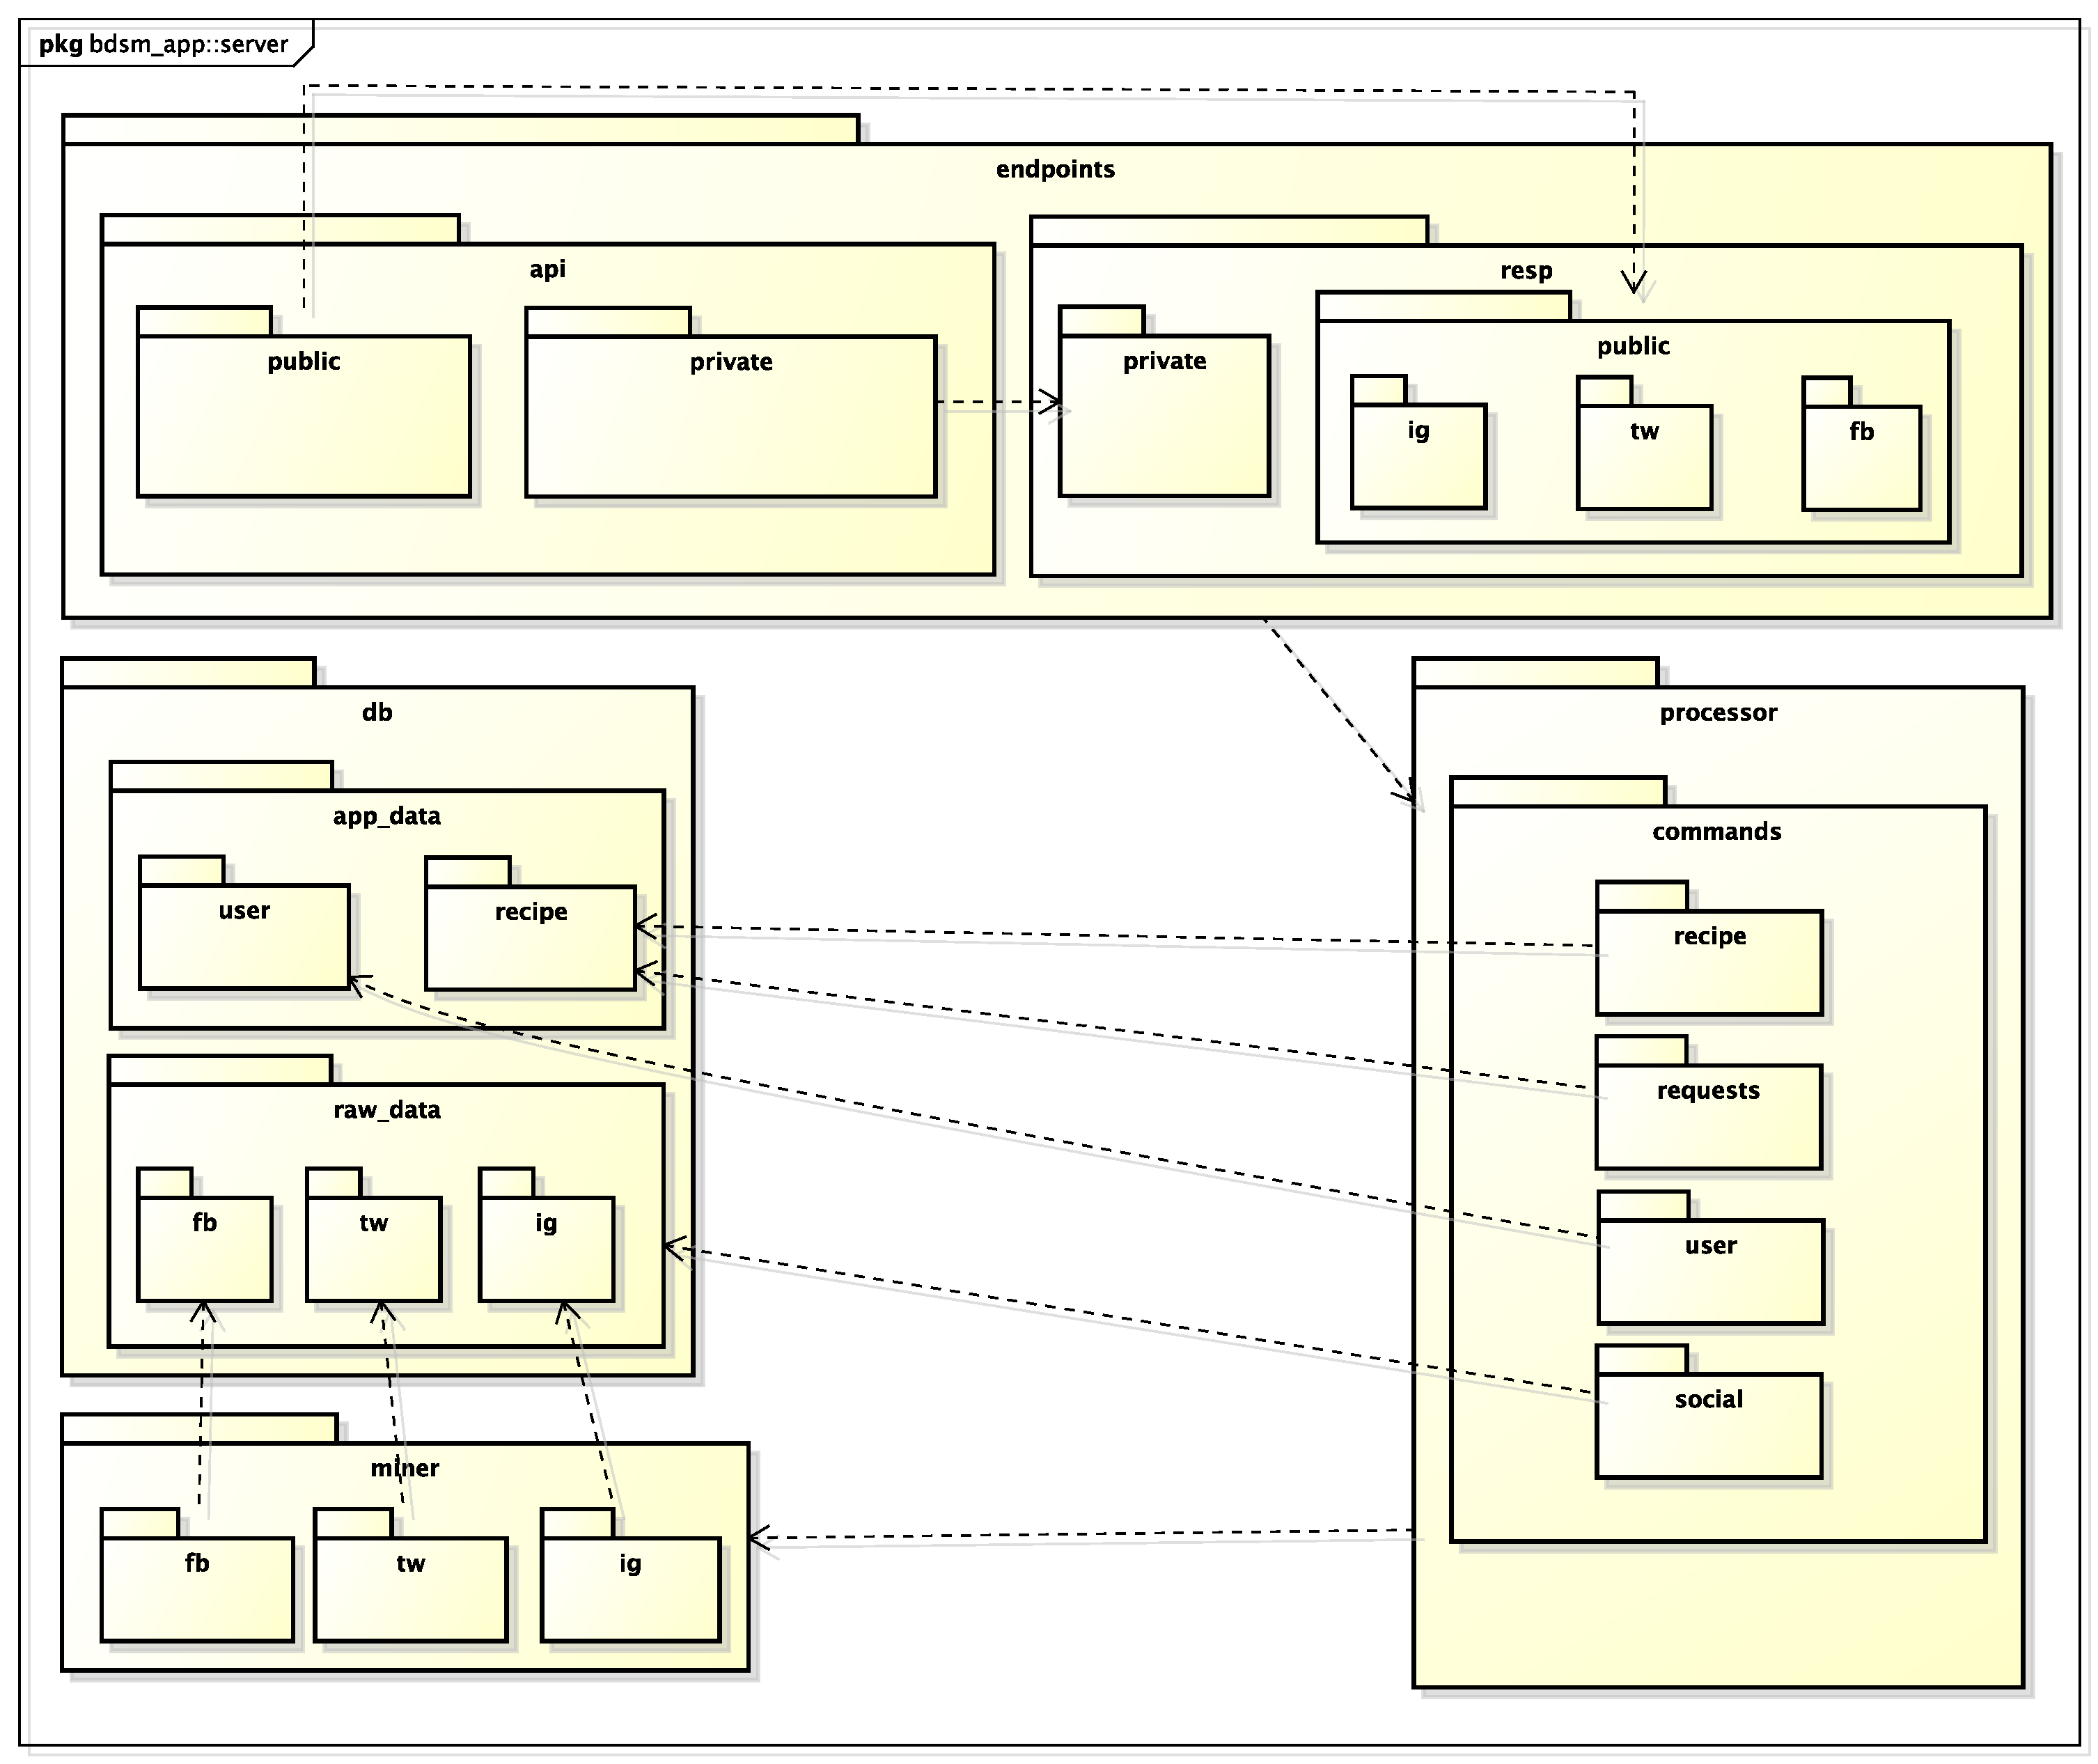
\includegraphics[scale=0.38]{./images/server/server.pdf}}
    \caption{Package - server}
  \end{figure}


  \begin{itemize}
    \item \textbf{Descrizione}: è il package che racchiude tutte le parti del back-end. \'E quindi l'insieme dei componenti che si occupa di soddisfare le richieste provenienti dal front-end, interagire col database, raccogliere i dati provenienti dai social networks, elaborarli ed esporli attraverso servizi REST.
    \item \textbf{Package contenuti}:
      \begin{itemize}
        \item server::processor
        \item server::db
        \item server::miner
        \item server::endpoints
      \end{itemize}
    \item \textbf{Interazione con altri componenti}: interagisce con il client definito nella sezione \ref{sub:client} tramite i servizi REST offerti dal modulo in questione;
  \end{itemize}
  % subsubsection bdsm_app_client (end)

  \pagebreak

  % PACKAGE DELLA DB
  % =================================================================================================
% File:			server_tier/db.tex
% Description:	Definisce la sezione relativa al back-end dell'applicazione
% Created:		2015-04-07
% Author:		Cusinato Giacomo
% Email:		cusinato.giacomo@mashup-unipd.it
% =================================================================================================
% Modification History:
% Version		Modifier Date		Change											Author
% 0.0.1			2015-04-18			Modifica grafici e relative descrizioni			Luca Santacatterina
% =================================================================================================

% CONTENUTO DEL CAPITOLO

\subsubsection{server::db} % (fold)
\label{ssub:bdsm_app_server_db}

	\begin{figure}[htbp]
		\centering
		\centerline{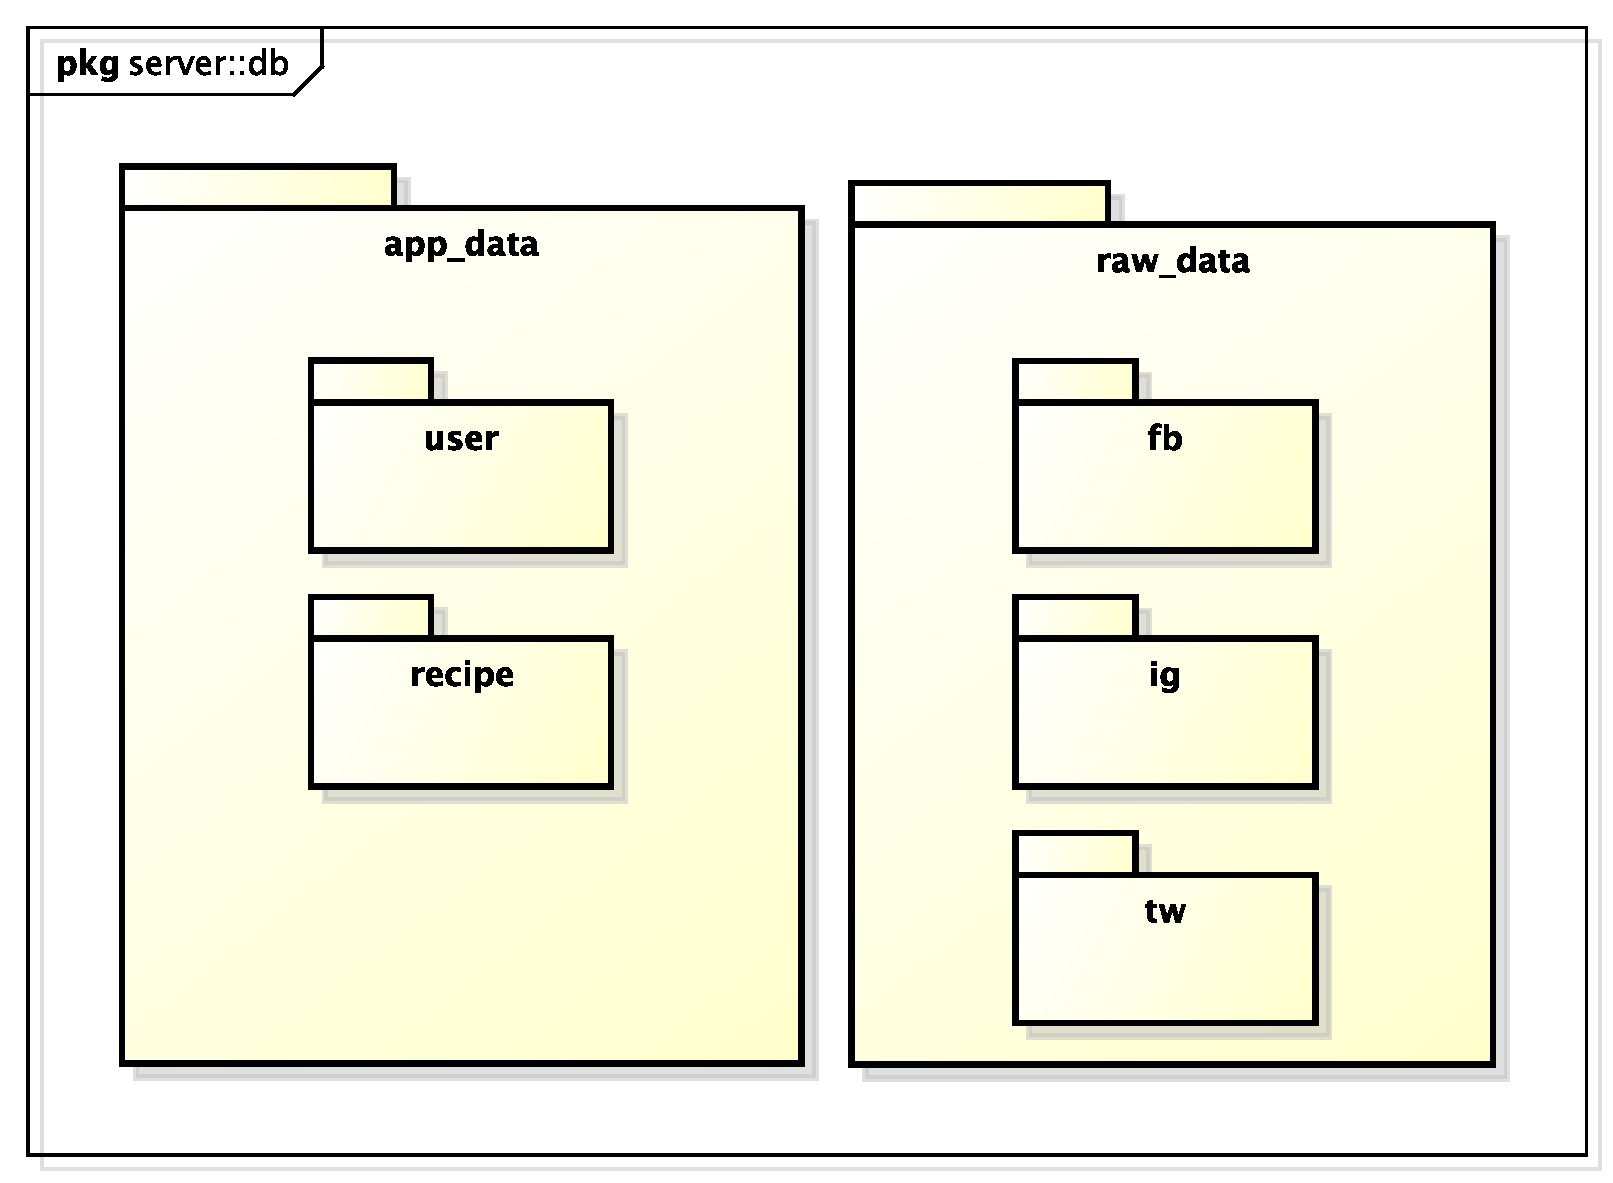
\includegraphics[scale=0.5]{./images/server/db.pdf}}
		\caption{Package - server::db}
	\end{figure}

	\begin{itemize}
		\item \textbf{Descrizione}: è il package che contiene le componenti che gestiscono e mantengono coerente la base di dati. Esse utilizzano standard proprietari Google per la loro implementazione. Sono suddivise in due package: uno atto a rappresentare il modello dei dati grezzi, l'altro dei parametri del software e degli utenti;
		\item \textbf{Padre}: server;
		\item \textbf{Package contenuti}:
			\begin{itemize}
				\item server::app\_data.
				\item server::raw\_data;
			\end{itemize}
	\end{itemize}



% subsubsection RAW_DATA
\subsubsection{server::db::raw\_data} % (fold)
\label{ssub:bdsm_app_server_raw_model}
	\begin{figure}[htbp]
		\centering
		\centerline{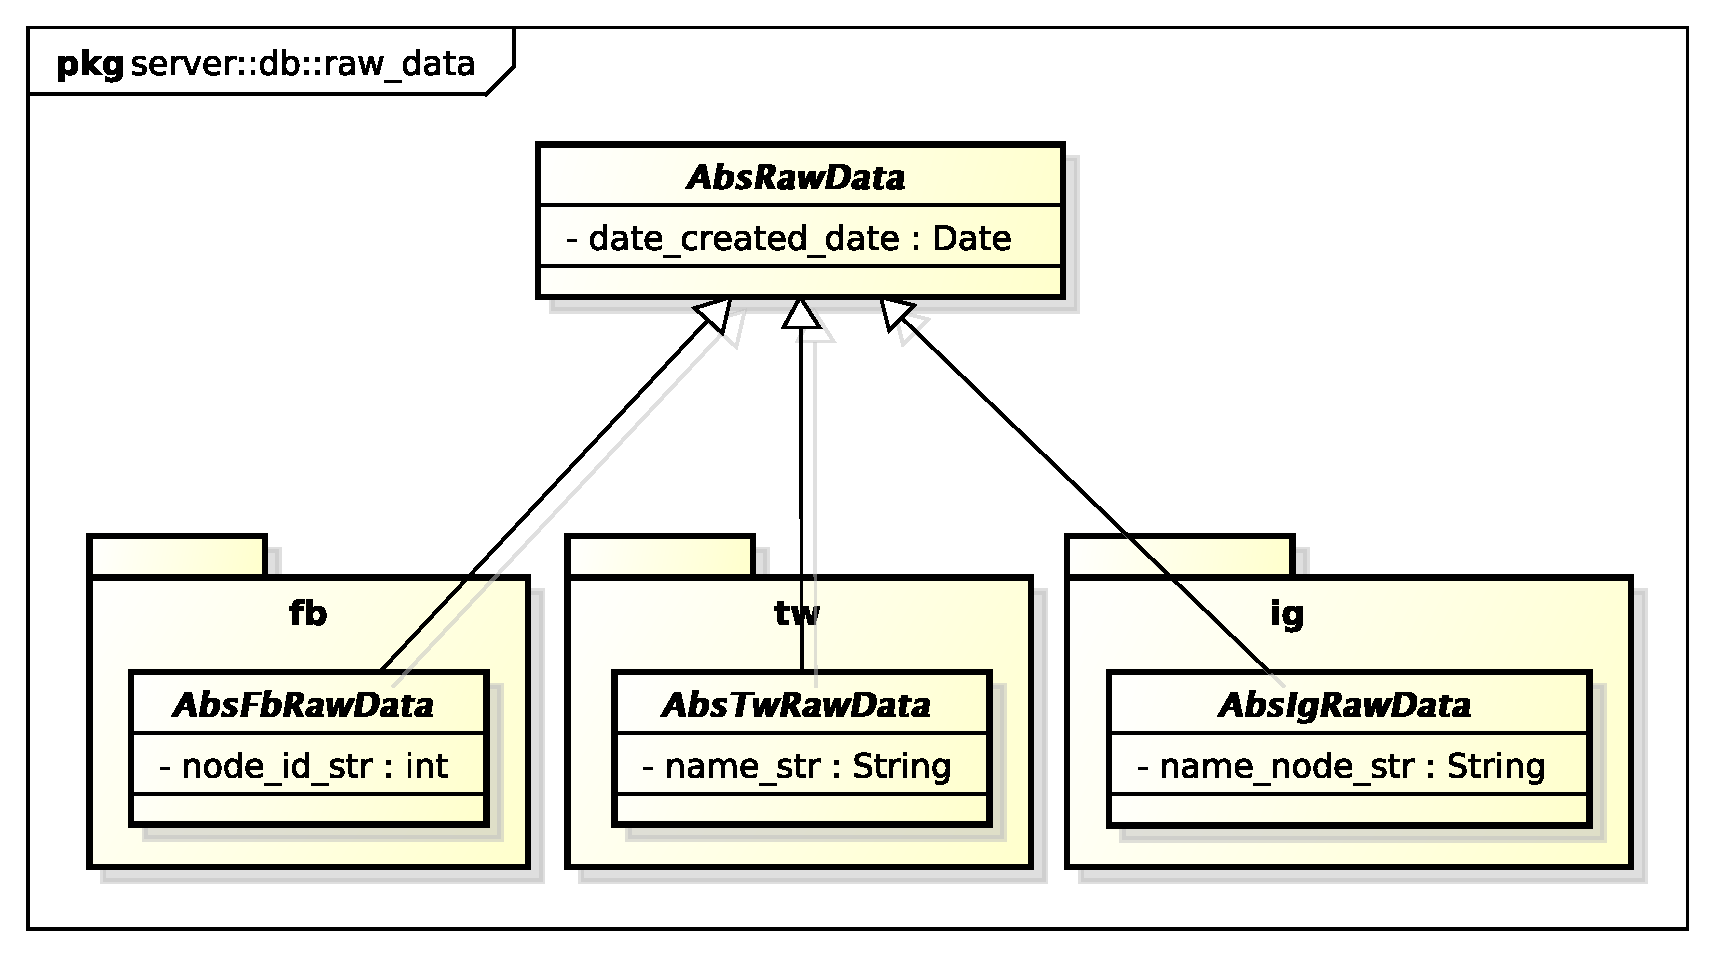
\includegraphics[scale=0.35]{./images/server/raw_data.pdf}}
		\caption{Package - server::db::raw\_data}
	\end{figure}

	\begin{itemize}
	\item \textbf{Descrizione}: package che definisce il modello dei dati grezzi ricavati dai vari social network;
		\item \textbf{Padre}: server::db;
		\item \textbf{Package contenuti}:
			\begin{itemize}
				\item server::db::raw\_data::fb
				\item server::db::raw\_data::tw
				\item server::db::raw\_data::ig
		\end{itemize}
	\end{itemize}


	\paragraph{Classi} % (fold)

		\subparagraph{server::db::raw\_model::AbsRawData} % (fold)
		\label{subp:bdsm_app_server_raw_model_absrawdata}
			\begin{itemize}
				\item \textbf{Descrizione}: classe astratta che definisce il modello di un dato grezzo;
				\item \textbf{Utilizzo}: la classe funge da padre per tutte le classi rappresentanti un dato grezzo;
				\item \textbf{Relazioni con altre classi}:
					\begin{itemize}
						\item AbsFbRawData
						\item AbsTwRawData
						\item AbsIgRawData
						\item RawFbPageTrend
						\item RawFbEventTrend
						\item RawFbPostTrend
						\item RawTwUserTrend
						\item RawTwHashtagTrend
						\item RawTwUserTweet
						\item RawIgUserTrend
						\item RawIgHashtagTrend
						\item RawIgMedia
					\end{itemize}
			\end{itemize}


		% subsubsection FACEBOOK
		\subsubsection{server::db::raw\_model::fb} % (fold)
		\label{ssub:bdsm_app_server_db_raw_model_fb}
		\begin{figure}[htbp]
			\centering
			\centerline{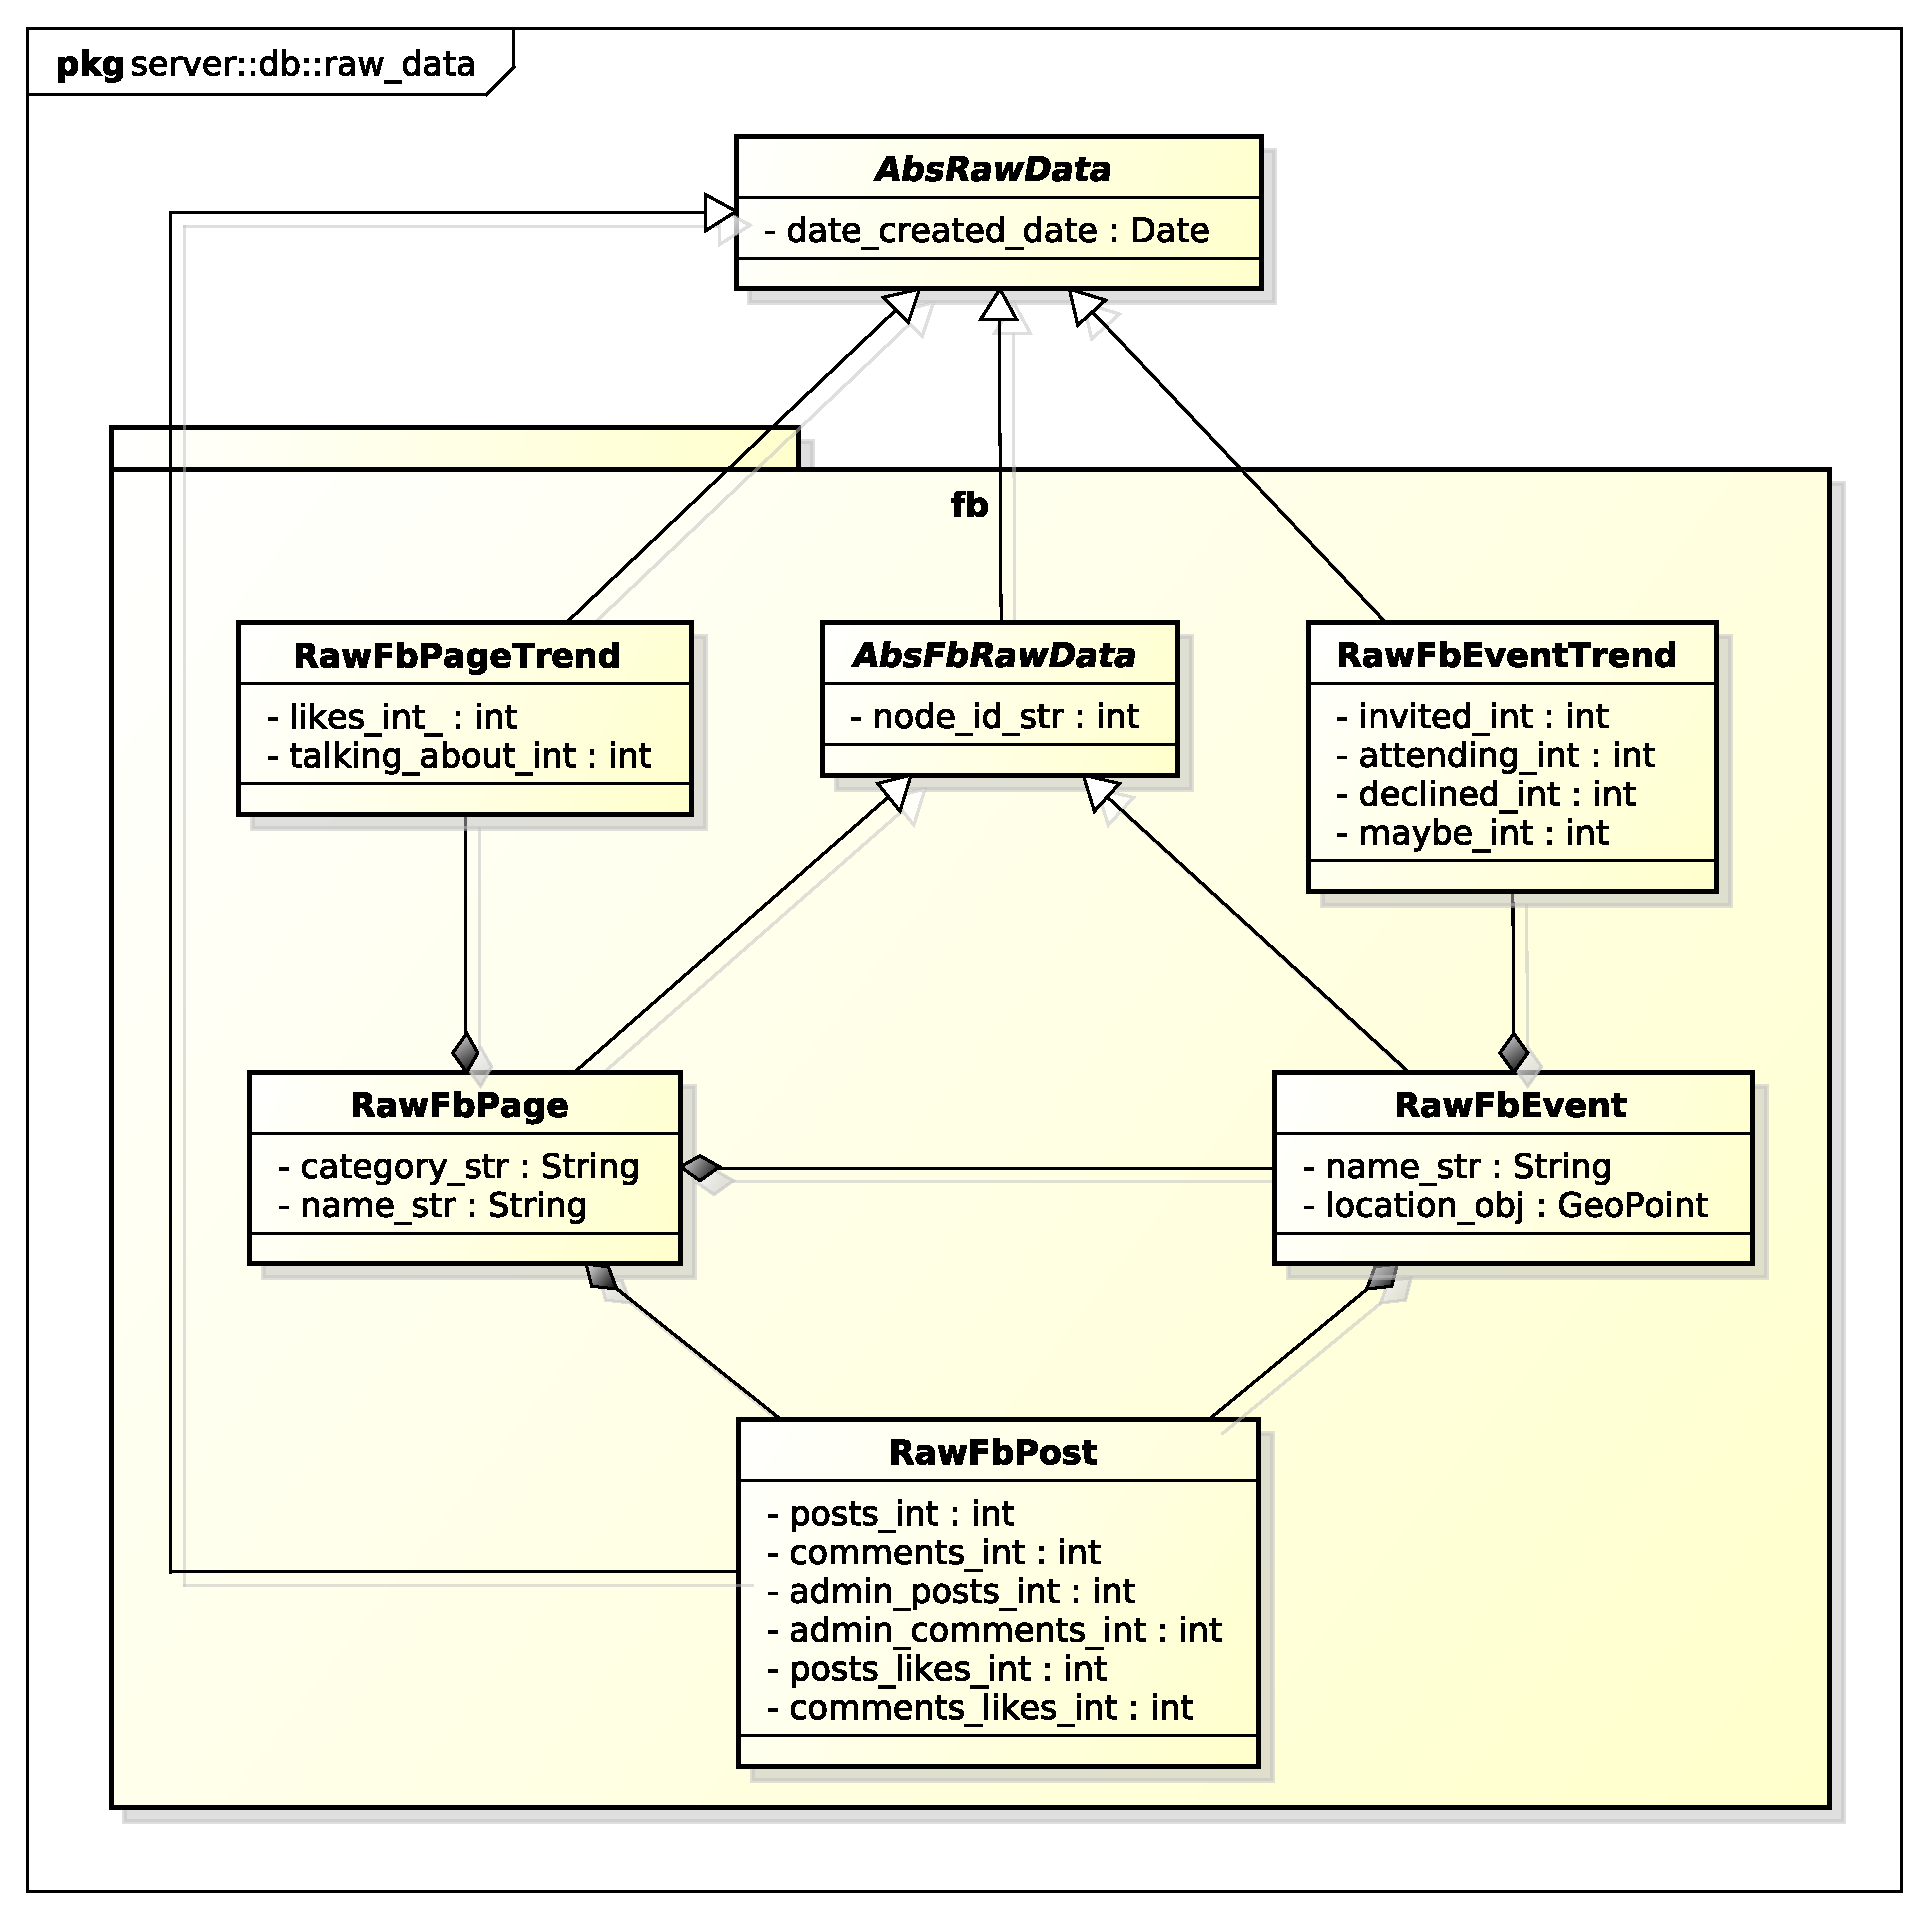
\includegraphics[scale=0.5]{./images/server/raw_data_fb.pdf}}
			\caption{Package - server::db::raw\_data::fb}
		\end{figure}

		\begin{itemize}
		  \item \textbf{Descrizione}:  è il package contenente le classi che definiscono i modelli dei dati grezzi relativi a Facebook;
		  \item \textbf{Padre}: server::db::raw\_model
		  \item \textbf{Interazione con altri componenti}:
		  	\begin{itemize}
		  		\item server::db
				\end{itemize}
		\end{itemize}
		% subsubsection

		\paragraph{Classi} % (fold)

			\subparagraph{server::db::raw\_data::fb::AbsFbRawData} % (fold)
			\label{subp:server_db_raw_data_fb_absfbrawdata}
				\begin{itemize}
					\item \textbf{Descrizione}: classe astratta che definisce il modello dati grezzi relativi a Facebook;
					\item \textbf{Utilizzo}: la classe contiene l'id fornito dall'utente il quale permette di identificare univocamente la risorsa nel social media;
					\item \textbf{Classi ereditate}: server::db::raw\_data::AbsRawData
				\end{itemize}
			% subparagraph server_db_raw_data_fb_absfbrawdata [end]


			\subparagraph{server::db::raw\_data::fb::RawFbPage} % (fold)
			\label{subp:server_db_raw_data_fb_rawfbpage}
				\begin{itemize}
					\item \textbf{Descrizione}: classe che rappresenta il modello di una pagina Facebook;
					\item \textbf{Utilizzo}: la classe fornisce metodi per memorizzare i dati statici di una pagina Facebook;
					\item \textbf{Classi ereditate}: server::db::raw\_data::AbsFbRawData
					\item \textbf{Relazioni con altre classi}:
						\begin{itemize}
							\item server::db::raw\_data::fb::RawFbEvent
							\item server::db::raw\_data::fb::RawFbPageTrend
							\item server::db::raw\_data::fb::RawFbPost
						\end{itemize}
				\end{itemize}
			% subparagraph server_db_raw_data_fb_rawfbpage [end]

			\subparagraph{server::db::raw\_data::fb::RawFbPageTrend} % (fold)
			\label{subp:server_db_raw_data_fb_rowfbpagetrend}
				\begin{itemize}
					\item \textbf{Descrizione}: classe che rappresenta il modello del trend dei dati una pagina Facebook;
					\item \textbf{Utilizzo}: la classe viene utilizzata per memorizzare e il numero di like e di talking about di ogni singola pagina;
					\item \textbf{Classi ereditate}: server::db::raw\_data::AbsRawData
				\end{itemize}
			% subparagraph server_db_raw_data_fb_rowfbpagetrend [end]


			\subparagraph{server::db::raw\_data::fb::RawFbEvent} % (fold)
			\label{subp:server_db_raw_data_fb_rawfbevent}
				\begin{itemize}
					\item \textbf{Descrizione}: classe che rappresenta il modello di un evento Facebook;
					\item \textbf{Utilizzo}: la classe fornisce metodi per memorizzare i dati statici di un evento Facebook;
					\item \textbf{Classi ereditate}: server::db::raw\_data::AbsFbRawData
					\item \textbf{Relazioni con altre classi}:
						\begin{itemize}
							\item server::db::raw\_data::fb::RawFbEventTrend
							\item server::db::raw\_data::fb::RawFbPost
						\end{itemize}
				\end{itemize}
			% subparagraph server_db_raw_data_fb_rawfbevent [end]


			\subparagraph{server::db::raw\_data::fb::RawFbEventTrend} % (fold)
			\label{subp:server_db_raw_data_fb_rowfbeventtrend}
				\begin{itemize}
					\item \textbf{Descrizione}: classe che rappresenta il modello del trend di un evento su Facebook;
					\item \textbf{Utilizzo}: la classe viene utilizzata per memorizzare il numero di utenti invitati, partecipanti e non di un evento;
					\item \textbf{Classi ereditate}: server::db::raw\_data::AbsRawData
				\end{itemize}
			% subparagraph server_db_raw_data_fb_rowfbeventtrend [end]


			\subparagraph{server::db::raw\_data::fb::RawFbPost} % (fold)
			\label{subp:server_db_raw_data_fb_rawfbpost}
				\begin{itemize}
					\item \textbf{Descrizione}: classe che rappresenta il modello del trend dei post di una pagina o di un evento su Facebook;
					\item \textbf{Utilizzo}: la classe fornisce metodi per sommare i dati statici sui post di Facebook;
				\end{itemize}
			% subparagraph server_db_raw_data_fb_rawfbpost [end]


		% subsubsection INSTAGRAM
		\subsubsection{server::db::raw\_model::ig} % (fold)
		\label{ssub:bdsm_app_server_db_raw_model_ig}
		\begin{figure}[htbp]
			\centering
			\centerline{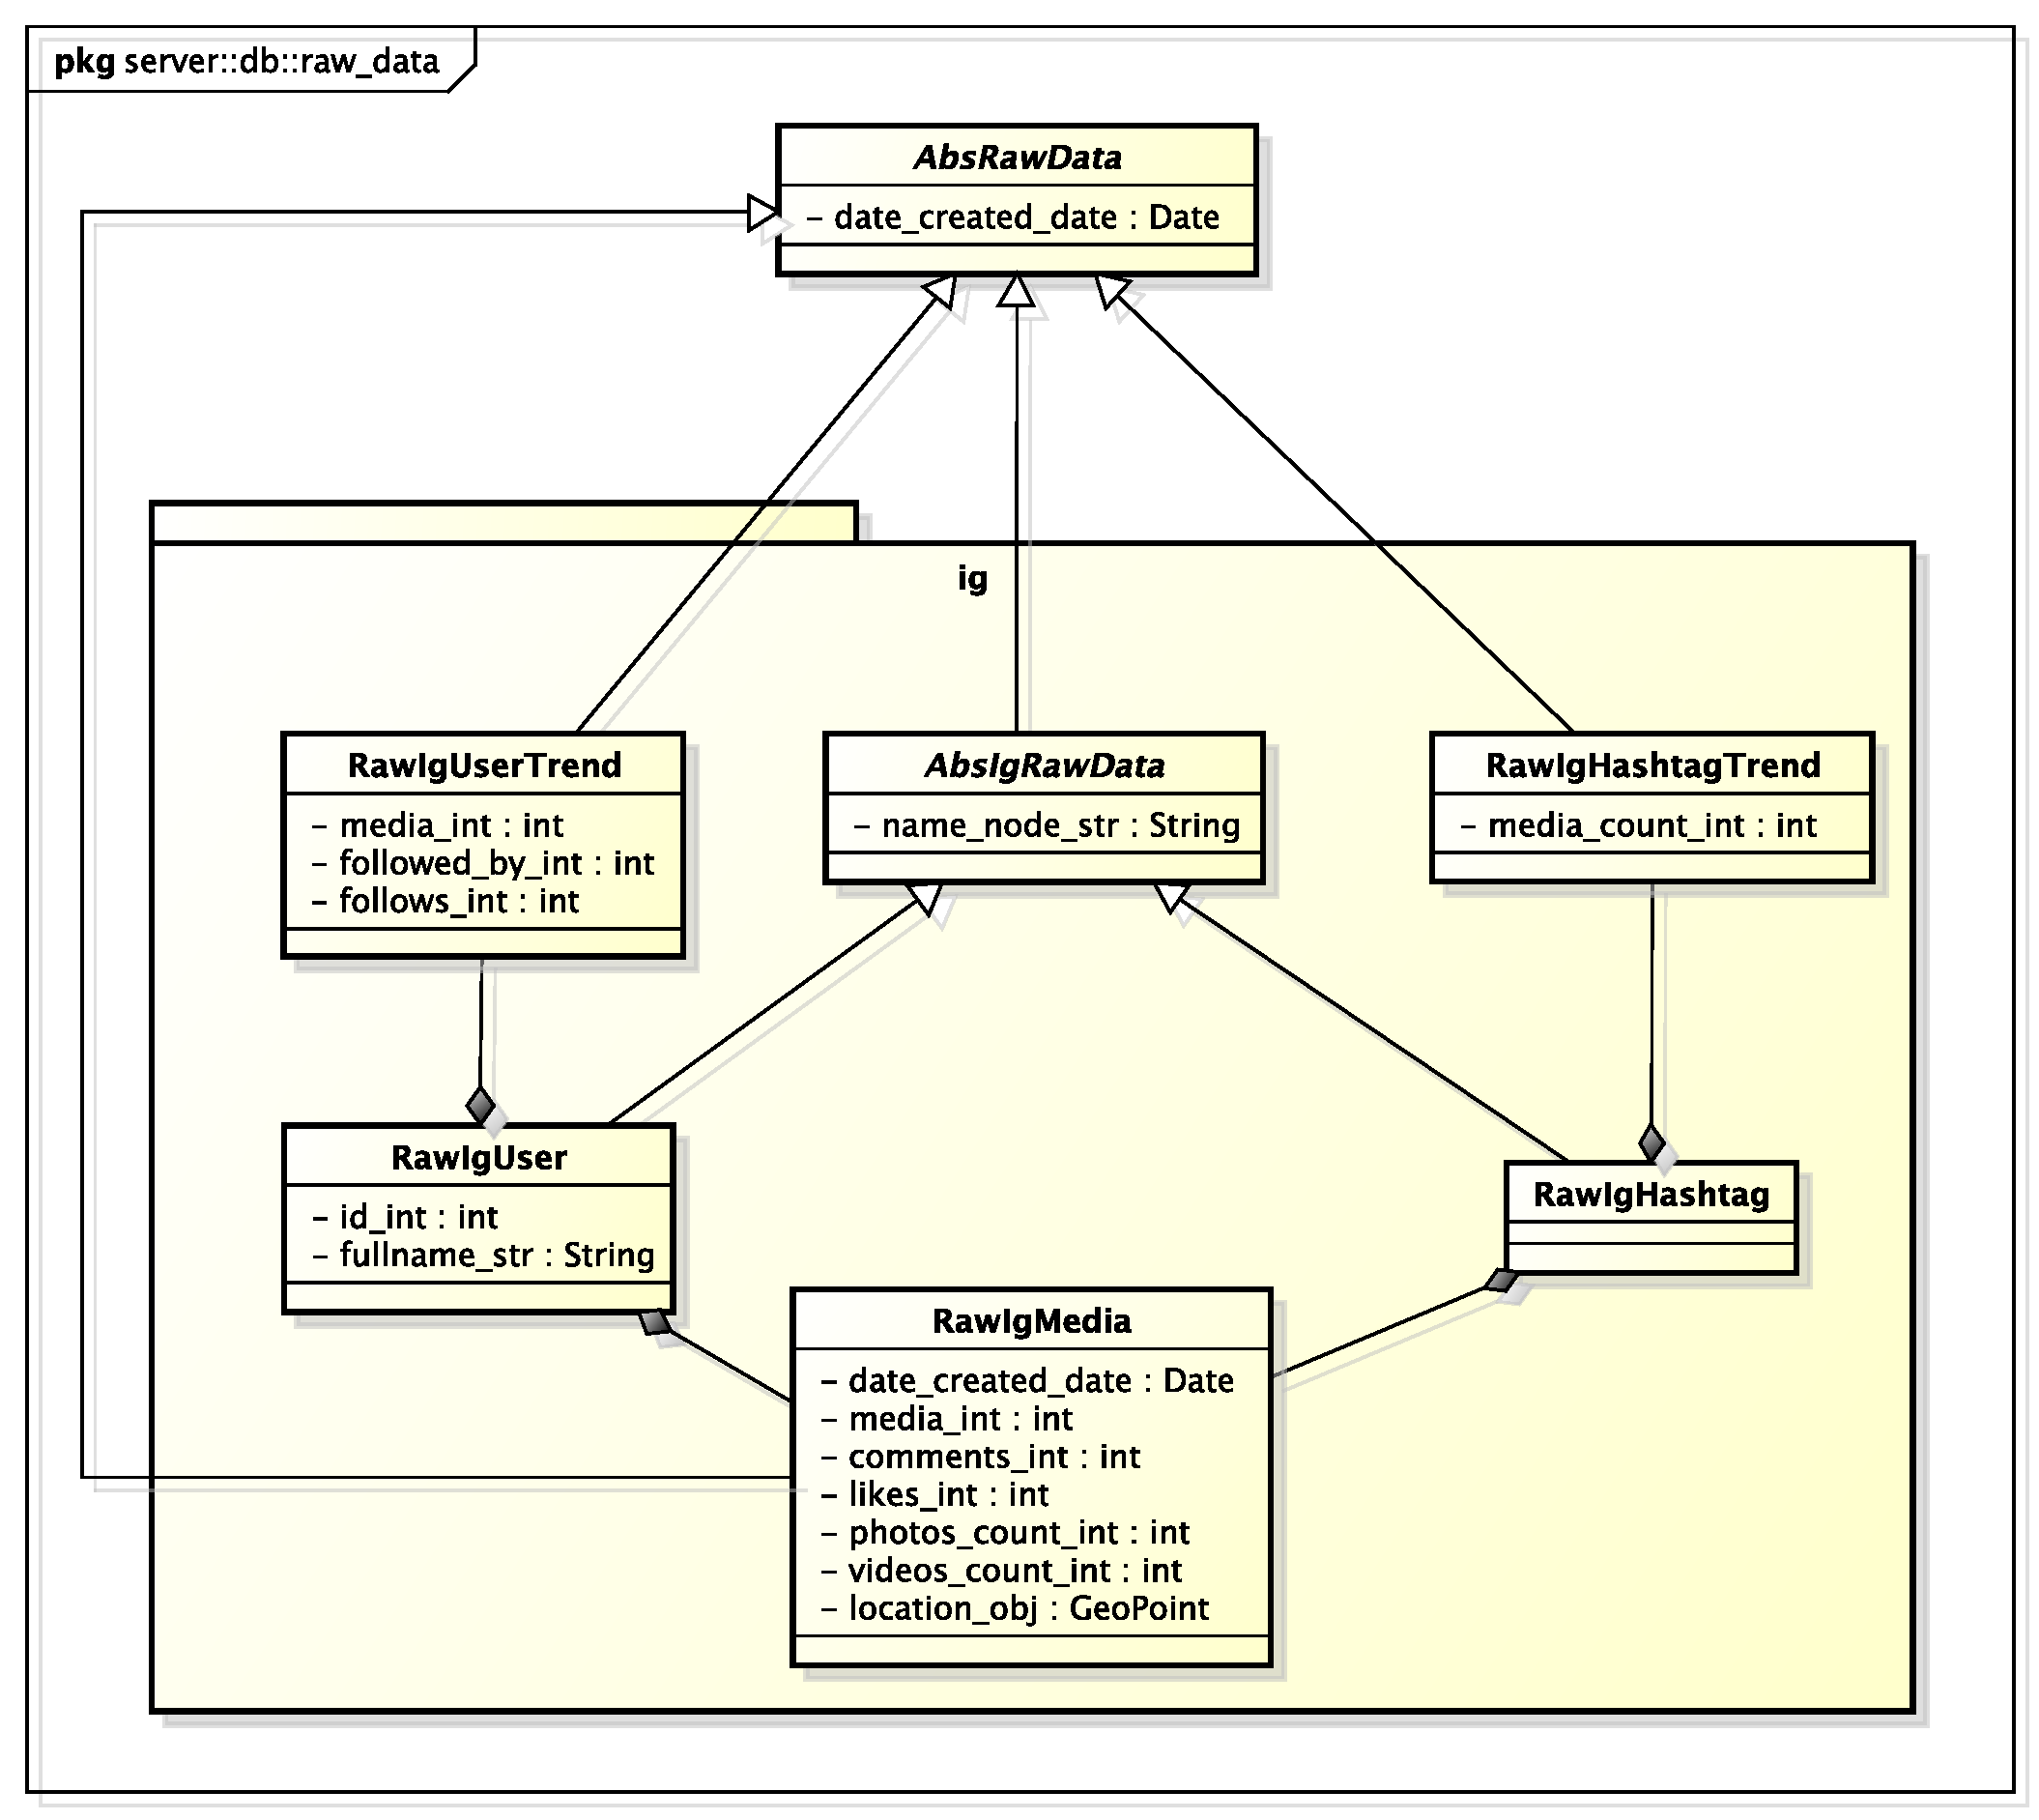
\includegraphics[scale=0.5]{./images/server/raw_data_ig.pdf}}
			\caption{Package - server::db::raw\_data::ig}
		\end{figure}

		\begin{itemize}
		  \item \textbf{Descrizione}: è il package contenente le classi che definiscono i modelli dei dati grezzi relativi a Instagram;
		  \item \textbf{Padre}: server::db::raw\_model
		  \item \textbf{Interazione con altri componenti}:
		  	\begin{itemize}
		  		\item server::db
				\end{itemize}
		\end{itemize}
		% subsubsection

		\paragraph{Classi} % (fold)


		\subparagraph{server::db::raw\_data::ig::AbsIgRawData} % (fold)
		\label{subp:server_db_raw_data_ig_absigrawdata}
			\begin{itemize}
				\item \textbf{Descrizione}: classe astratta che definisce il modello dei dati grezzi realtivi ad Instagram;
				\item \textbf{Utilizzo}: la classe contiene l'id fornito dall'utente il quale permette di identificare univocamente la risorsa nel social media;
				\item \textbf{Classi ereditate}: server::db::raw\_data::AbsRawData
			\end{itemize}
		% subparagraph server_db_raw_data_ig_absigrawdata [end]


		\subparagraph{server::db::raw\_data::ig::RawIgUser} % (fold)
		\label{subp:server_db_raw_data_ig_rawiguser}
			\begin{itemize}
				\item \textbf{Descrizione}: classe che definisce il modello dei dati di un utente Instagram;
				\item \textbf{Utilizzo}:  la classe viene utilizzata per memorizzare le i dettagli di un utente Instagram;
				\item \textbf{Classi ereditate}: server::db::raw\_data::AbsIgRawData
				\item \textbf{Relazioni con altre classi}:
					\begin{itemize}
						\item server::db::raw\_data::ig::RawIgUserTrend
						\item server::db::raw\_data::ig::RawIgMedia
					\end{itemize}
			\end{itemize}
		% subparagraph server_db_raw_data_ig_rawiguser [end]


		\subparagraph{server::db::raw\_data::ig::RawIgUserTrend} % (fold)
		\label{subp:server_db_raw_data_ig_rawigusertrend}
			\begin{itemize}
				\item \textbf{Descrizione}: classe che definisce il modello dei dati del trend di un utente Instagram;
				\item \textbf{Utilizzo}: la classe viene utilizzata per memorizzare il numero di media, di followed e follows di una determinata persona;
				\item \textbf{Classi ereditate}: server::db::raw\_data::AbsRawData
			\end{itemize}
		% subparagraph server_db_raw_data_ig_rawigusertrend [end]


		\subparagraph{server::db::raw\_data::ig::RawIgHashtag} % (fold)
		\label{subp:server_db_raw_data_ig_rawighashtag}
			\begin{itemize}
				\item \textbf{Descrizione}: classe che definisce il modello dei dati di un hashtag Instagram;
				\item \textbf{Utilizzo}: la classe viene utilizzata per fornire una descrizione minimale dell'hashtag su Instagram;
				\item \textbf{Classi ereditate}: server::db::raw\_data::AbsIgRawData
				\item \textbf{Relazioni con altre classi}:
					\begin{itemize}
						\item server::db::raw\_data::ig::RawIgHashtagTrend
						\item server::db::raw\_data::ig::RawIgMedia
					\end{itemize}
			\end{itemize}
		% subparagraph server_db_raw_data_ig_rawighashtag [end]


		\subparagraph{server::db::raw\_data::ig::RawIgHashtagTrend} % (fold)
		\label{subp:server_db_raw_data_ig_rawighashtagtrend}
			\begin{itemize}
				\item \textbf{Descrizione}: classe che definisce il modello dei dati del trend di un hastag Instagram;
				\item \textbf{Utilizzo}: la classe viene utilizzata per memorizzare il numero di media caricati di un determinato hashtag;
				\item \textbf{Classi ereditate}: server::db::raw\_data::AbsRawData
			\end{itemize}
		% subparagraph server_db_raw_data_ig_rawighashtagtrend [end]


		\subparagraph{server::db::raw\_data::ig::RawIgMedia} % (fold)
		\label{subp:server_db_raw_data_ig_rawigmedia}
			\begin{itemize}
				\item \textbf{Descrizione}: classe che definisce il modello dei dati di un media realtivo ad Instagram;
				\item \textbf{Utilizzo}: la classe viene utilizzata per fornire una descrizione dettagliata di un media caricato da un utente specifico su Instagram. Vengono forniti metodi automatici per il conteggio dei parametri che verranno utilizzati per seguire un trend;
				\item \textbf{Classi ereditate}: server::db::raw\_data::AbsRawData
			\end{itemize}
		% subparagraph server_db_raw_data_ig_rawigmedia [end]


		% subsubsection TWITTER
		\subsubsection{bdsm\_app::server::db::raw\_model::tw} % (fold)
		\label{ssub:bdsm_app_server_db_raw_model_tw}
		\begin{figure}[htbp]
			\centering
			\centerline{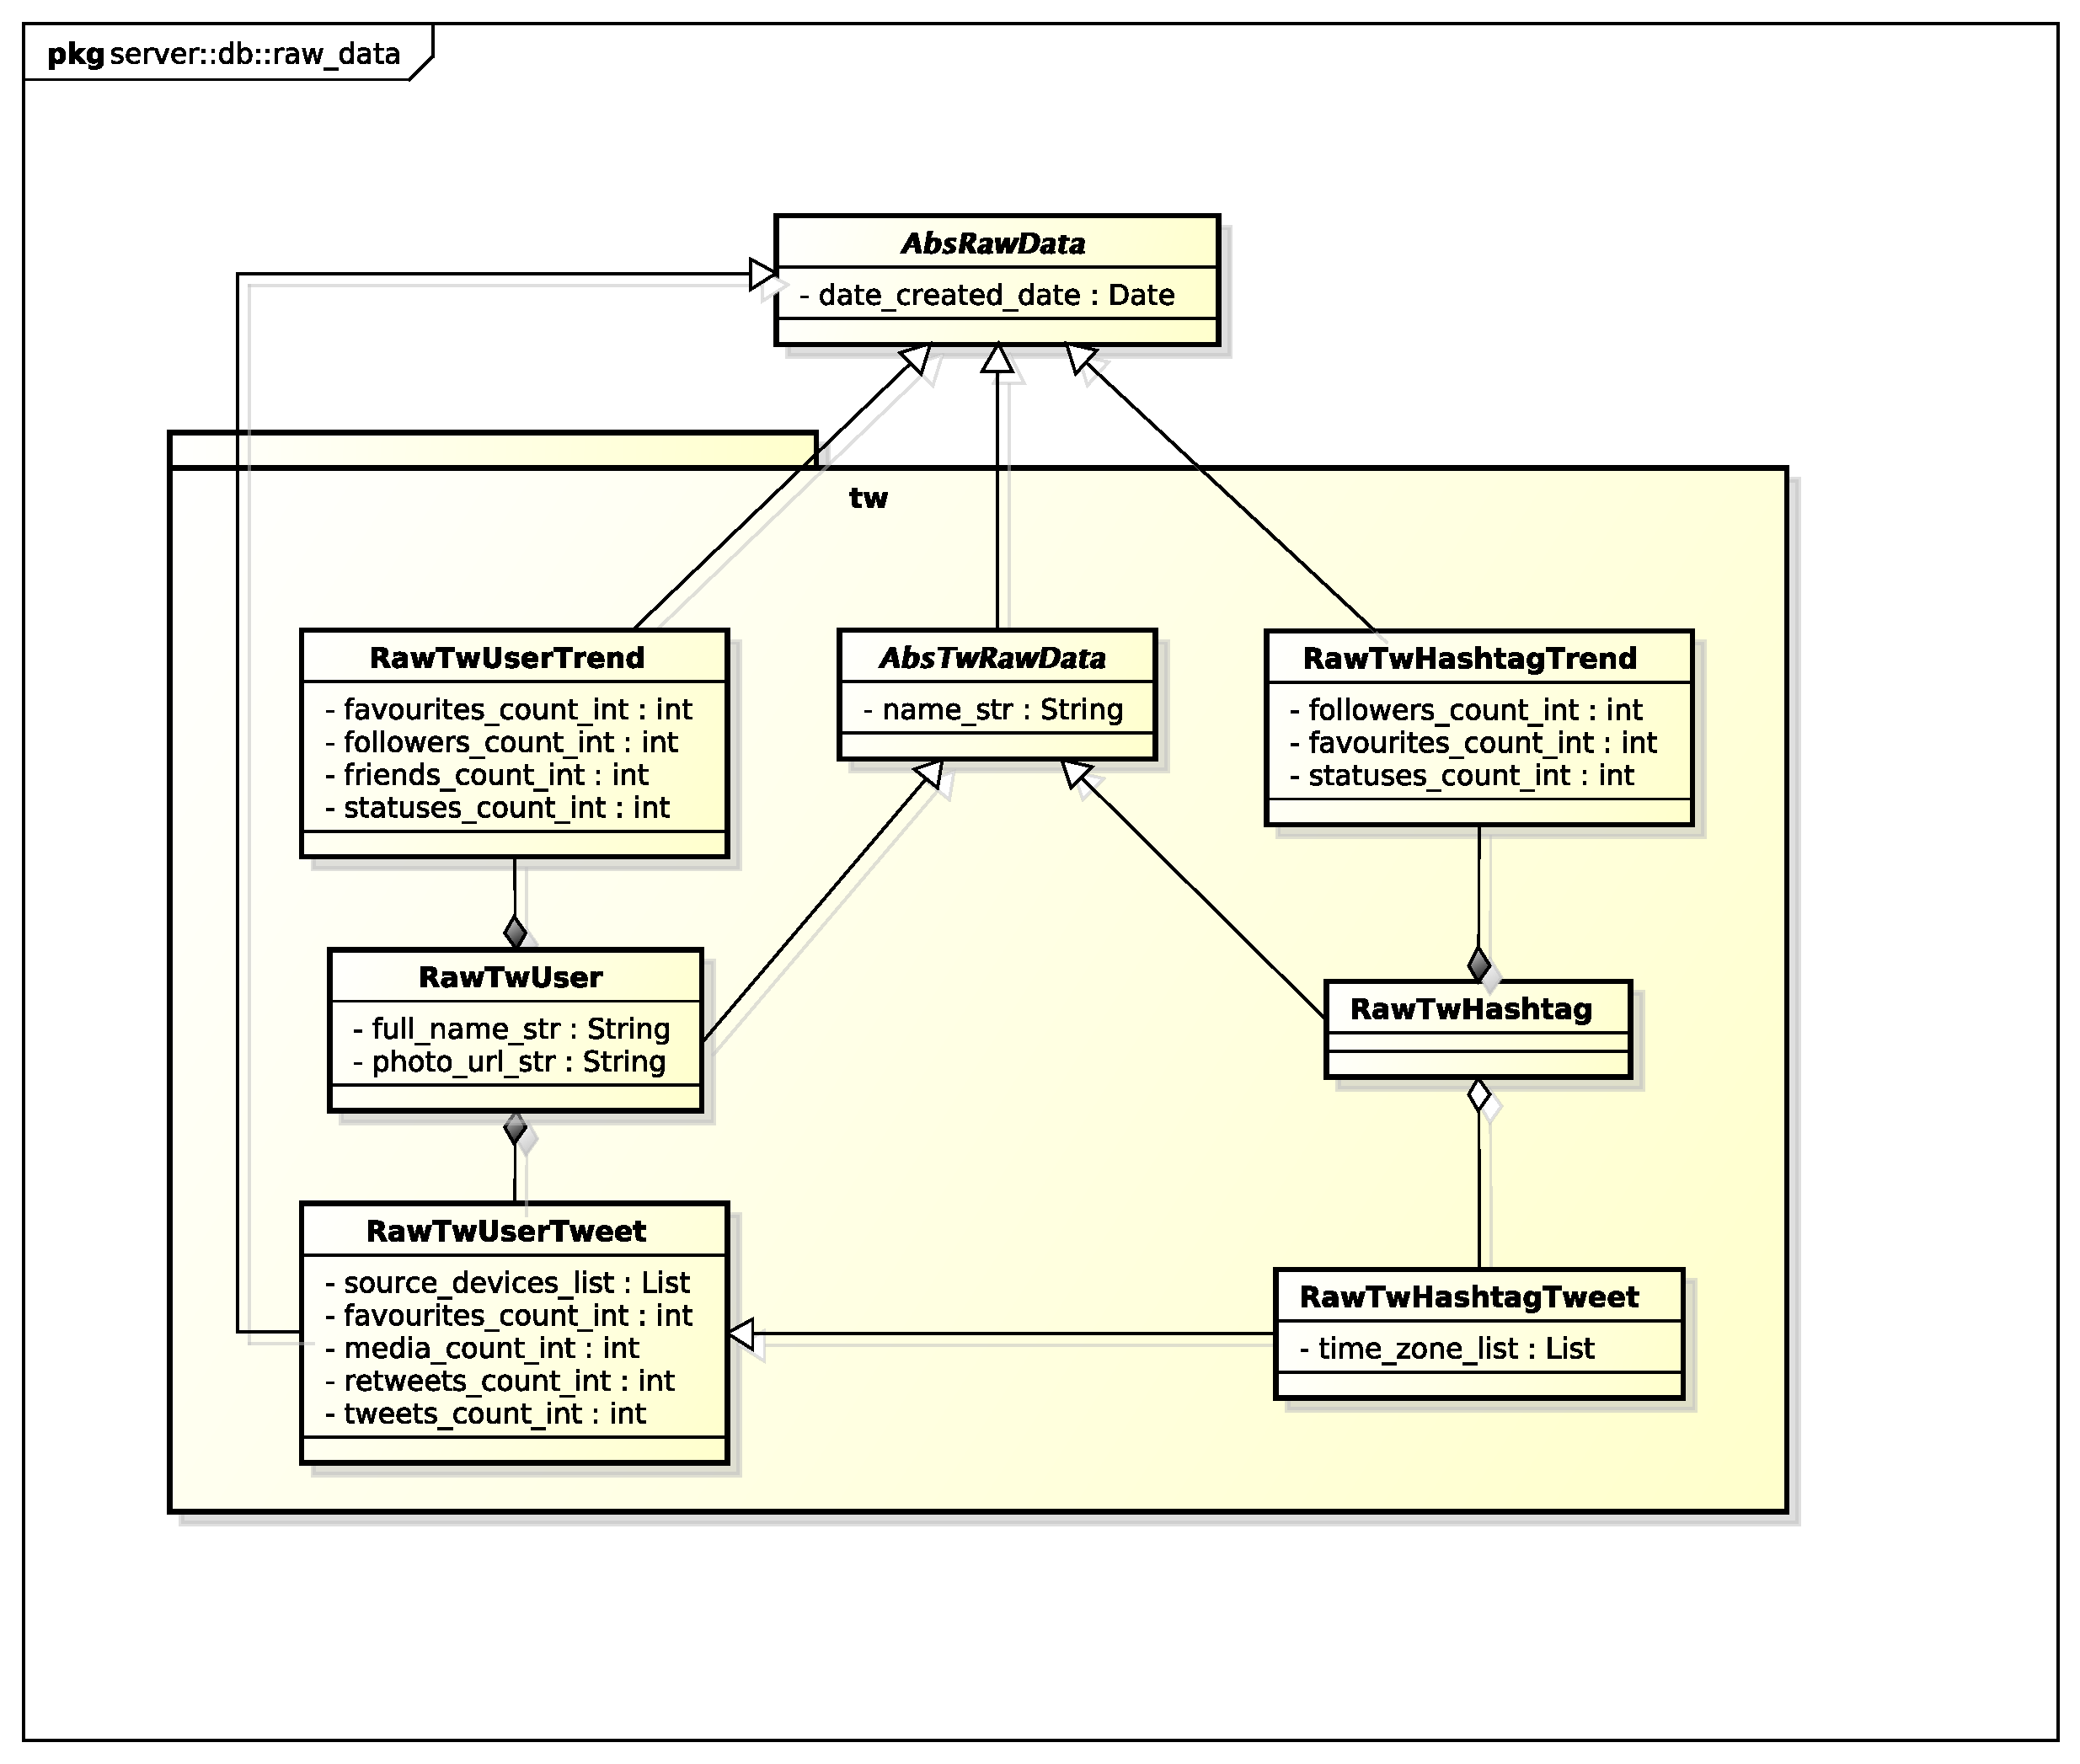
\includegraphics[scale=0.45]{./images/server/raw_data_tw.pdf}}
			\caption{Package - server::db::raw\_data::tw}
		\end{figure}

		\begin{itemize}
		  \item \textbf{Descrizione}: è il package contenente le classi che definiscono i modelli dei dati grezzi relativi a Twitter;
		  \item \textbf{Padre}: server::db::raw\_model
		  \item \textbf{Interazione con altri componenti}:
		  	\begin{itemize}
		  		\item server::db
				\end{itemize}
		\end{itemize}
		% subsubsection

		\paragraph{Classi} % (fold)


		\subparagraph{server::db::raw\_data::tw::AbsTwRawData} % (fold)
		\label{subp:server_db_raw_data_tw_abstwrawdata}
			\begin{itemize}
				\item \textbf{Descrizione}: classe astratta che definisce il modello dati grezzi realtivi a Twitter;
				\item \textbf{Utilizzo}: la classe contiene l'id fornito dall'utente il quale permette di identificare univocamente la risorsa nel social media;
				\item \textbf{Classi ereditate}: server::db::raw\_data::AbsRawData
			\end{itemize}
		% subparagraph server_db_raw_data_tw_abstwrawdata [end]


		\subparagraph{server::db::raw\_data::tw::RawTwUser} % (fold)
		\label{subp:server_db_raw_data_tw_rawtwuser}
			\begin{itemize}
				\item \textbf{Descrizione}: classe che definisce il modello dei dati di un utente Twitter;
				\item \textbf{Utilizzo}: la classe viene utilizzata per fornire una descrizione completa dell'utente Twitter. Vengono forniti metodi automatici per il conteggio dei parametri che verranno utilizzati per seguire un trend;;
				\item \textbf{Classi ereditate}: server::db::raw\_data::AbsTwRawData
				\item \textbf{Relazioni con altre classi}:
					\begin{itemize}
						\item server::db::raw\_data::tw::RawTwUserTrend
						\item server::db::raw\_data::tw::RawTwUserTweet
					\end{itemize}
			\end{itemize}
		% subparagraph server_db_raw_data_tw_rawtwuser [end]


		\subparagraph{server::db::raw\_data::tw::RawTwUserTrend} % (fold)
		\label{subp:server_db_raw_data_tw_rawigusertrend}
			\begin{itemize}
				\item \textbf{Descrizione}: classe che definisce il modello dei dati del trend di un utente Twitter;
				\item \textbf{Utilizzo}: la classe viene utilizzata per memorizzare il numero di favoriti, di followers, di friends e statuses di una determinata persona;
				\item \textbf{Classi ereditate}: server::db::raw\_data::AbsTwRawData
			\end{itemize}
		% subparagraph server_db_raw_data_tw_rawigusertrend [end]


		\subparagraph{server::db::raw\_data::tw::RawTwUserTweet} % (fold)
		\label{subp:server_db_raw_data_tw_rawtwusertweet}
			\begin{itemize}
				\item \textbf{Descrizione}: classe che definisce il modello dei dati del trend dei tweet relativi ad un utente Twitter;
				\item \textbf{Utilizzo}: la classe viene utilizzata per fornire una descrizione dettagliata di un tweet creato da un utente specifico su Twitter;
				\item \textbf{Classi ereditate}: server::db::raw\_data::AbsRawData
			\end{itemize}
		% subparagraph server_db_raw_data_tw_rawtwusertweet [end]


		\subparagraph{server::db::raw\_data::tw::RawTwHashtag} % (fold)
		\label{subp:server_db_raw_data_tw_rawtwhashtag}
			\begin{itemize}
				\item \textbf{Descrizione}: classe che definisce il modello dei dati di un hashtag su Twitter;
				\item \textbf{Utilizzo}: la classe viene utilizzata per fornire una descrizione minimale di un hashtag su Twitter. Vengono forniti metodi automatici per il conteggio dei parametri che verranno utilizzati per seguire un trend;
				\item \textbf{Classi ereditate}: server::db::raw\_data::AbsTwRawData
				\item \textbf{Relazioni con altre classi}:
					\begin{itemize}
						\item server::db::raw\_data::tw::RawTwHashtagTrend
						\item server::db::raw\_data::tw::RawTwHashtagTweet
					\end{itemize}
			\end{itemize}
		% subparagraph server_db_raw_data_tw_rawtwhashtag [end]


		\subparagraph{server::db::raw\_data::tw::RawTwHashtagTrend} % (fold)
		\label{subp:server_db_raw_data_tw_rawighashtagtrend}
			\begin{itemize}
				\item \textbf{Descrizione}: classe che definisce il modello dei dati del trend di un hashtag su Twitter;
				\item \textbf{Utilizzo}: la classe viene utilizzata per memorizzare il numero di favoriti, di followers e statuses di un determinato hashtag;
				\item \textbf{Classi ereditate}: server::db::raw\_data::AbsTwRawData
			\end{itemize}
		% subparagraph server_db_raw_data_tw_rawighashtagtrend [end]


		\subparagraph{server::db::raw\_data::tw::RawTwHashtagTweet} % (fold)
		\label{subp:server_db_raw_data_tw_rawtwhashtagtweet}
			\begin{itemize}
				\item \textbf{Descrizione}: classe che definisce il modello dei dati del trend dei tweet relativi ad un hashtag Twitter;
				\item \textbf{Utilizzo}: la classe viene utilizzata per fornire una descrizione della locazione spaziale di un tweet relativo all'hashtag su Twitter;
				\item \textbf{Classi ereditate}: server::db::raw\_data::RawTwUserTweet
			\end{itemize}
		% subparagraph server_db_raw_data_tw_rawtwhashtagtweet [end]





\subsubsection{bdsm\_app::server::db::app\_data} % (fold)
\label{ssub:bdsm_app_server_app_data}


	\begin{figure}[htbp]
		\centering
		\centerline{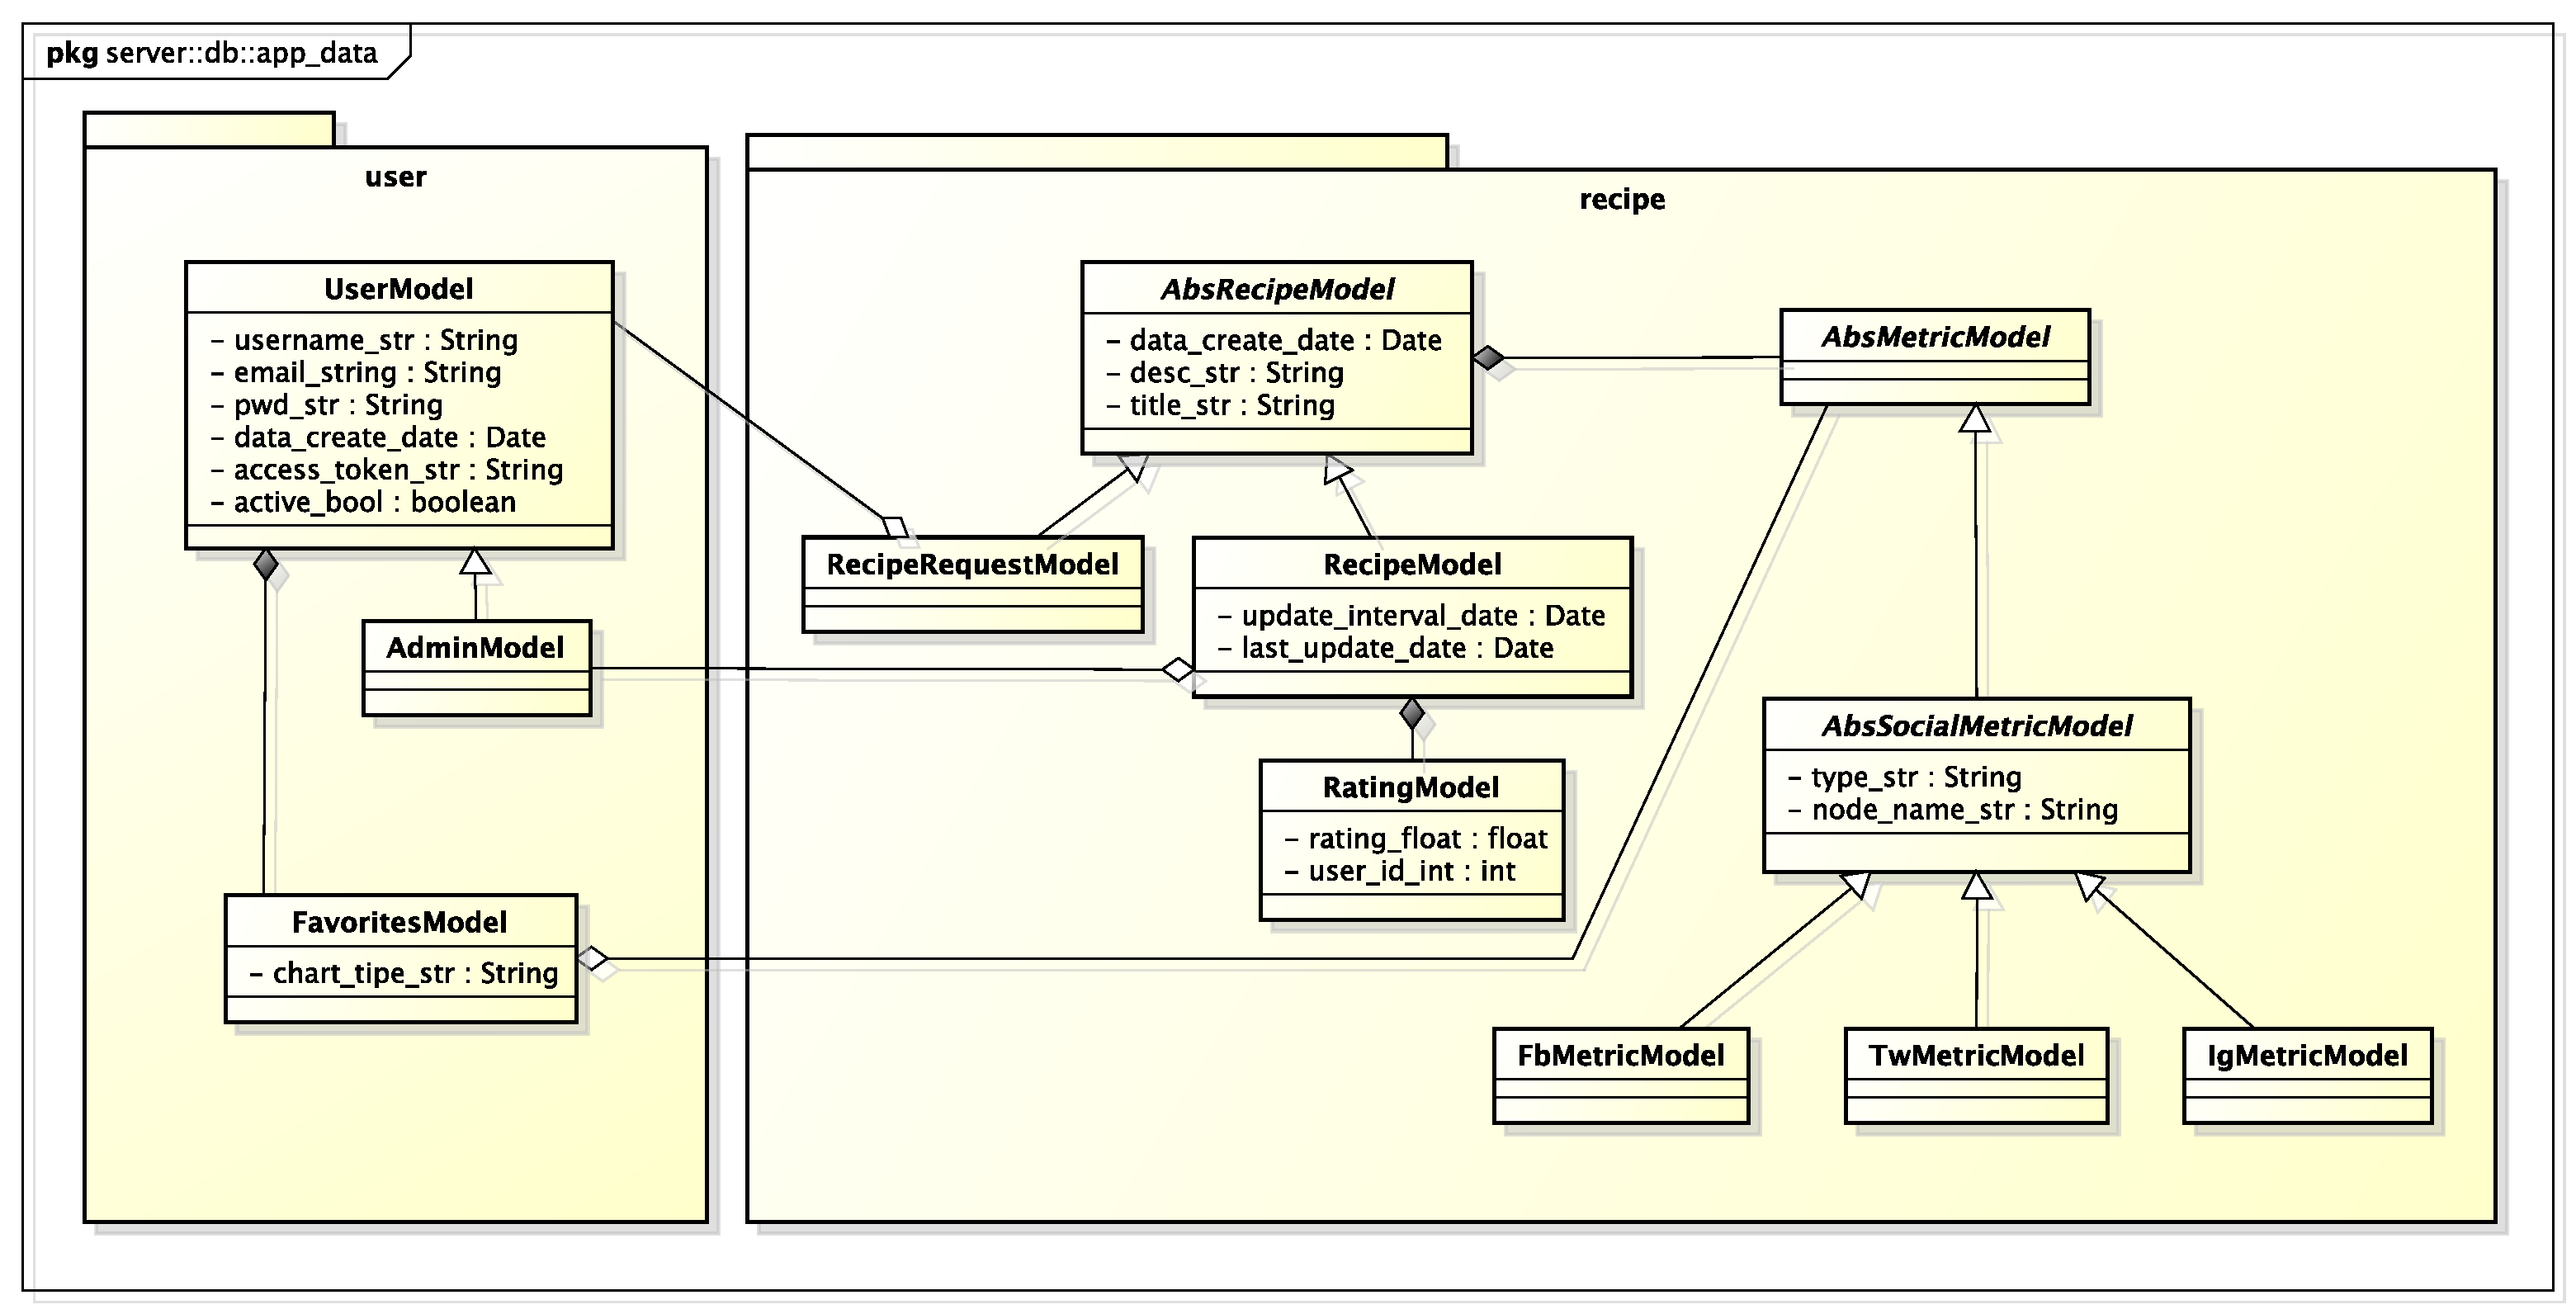
\includegraphics[scale=0.38]{./images/server/app_data.pdf}}
		\caption{Package - server::db::app\_data}
	\end{figure}


	\begin{itemize}
		\item \textbf{Descrizione}: è il package che contiene la definizione dei modelli degli utenti registrati e le loro preferenze. Contiene inoltre il modello delle Recipe che l'amministratore decide di creare;
		\item \textbf{Padre}: server::db
		\item \textbf{Package contenuti}
			\begin{itemize}
				\item server::db::app\_data::user
				\item server::db::app\_data::recipe
			\end{itemize}
		\item \textbf{Interazione con altri componenti}: interagisce con tutti i componenti del server in quanto fornisce i metodi per manipolare tutti i dati da memorizzare;
	\end{itemize}
	% subsubsection bdsm_app_server_app_data [end]


	\paragraph{Classi} % (fold)

		\subparagraph{server::db::app\_data::user::UserModel} % (fold)
		\label{subp:server_db_app_data_user_user_model}
			\begin{itemize}
				\item \textbf{Descrizione}: classe che definisce il modello dei dati degli utenti all'interno della base di dati;
				\item \textbf{Utilizzo}: la classe conterrà i metodi per la creazione, eliminazione, modifica degli account utente;
				\item \textbf{Relazioni con altre classi}:
					\begin{itemize}
						\item server::db::app\_data::user::FavouritesModel
						\item server::db:::app\_data::user::AdminModel
						\item server::db::app\_data::recipe::RecipeRequestModel
					\end{itemize}
			\end{itemize}
		% subparagraph server_db_app_data_user_user_model [end]


		\subparagraph{server::db::app\_data::user::AdminModel} % (fold)
		\label{subp:server_db_app_data_user_admin_model}
			\begin{itemize}
				\item \textbf{Descrizione}: classe che definisce il modello dei dati degli utenti amministratori all'interno della base di dati;
				\item \textbf{Utilizzo}: la classe specializza l'utente amministratore. Viene implementata con dei metodi per l'aggiunta la modifica e la rimozione;
				\item \textbf{Classi ereditate}: server::db::app\_data::user::UserModel;
				\item \textbf{Relazioni con altre classi}:
					\begin{itemize}
						\item server::db::app\_data::recipe::RecipeModel
					\end{itemize}
			\end{itemize}
		% subparagraph server_db_app_data_user_admin_model [end]


		\subparagraph{server::db::app\_data::user::FavouritesModel} % (fold)
		\label{subp:server_db_app_data_user_favorites}
			\begin{itemize}
				\item \textbf{Descrizione}: classe che definisce il modello dei dati ralativo ai preferiti dell'utente;
				\item \textbf{Utilizzo}: la classe  permette all'utente di aggiungere dei modelli di view nei preferiti. Contiene metodi per l'inserimento e rimozione di preferiti;
				\item \textbf{Relazioni con altre classi}:
					\begin{itemize}
						\item server::db::app\_data::recipe::AbsMetricModel
					\end{itemize}
			\end{itemize}
		% subparagraph server_db_app_data_user_favorites [end]


		\subparagraph{server::db::app\_data::recipe::AbsRecipeModel} % (fold)
		\label{subp:server_db_app_data_recipe_absrecipemodel}
			\begin{itemize}
				\item \textbf{Descrizione}: classe astratta che rappresenta un modello comune per Recipe e richiesta di aggiunta Recipe;
				\item \textbf{Utilizzo}: la classe mantiene l'estensibilità per eventuali nuovi tipi di Recipe;
				\item \textbf{Relazioni con altre classi}:
					\begin{itemize}
						\item server::db::app\_data::recipe::RecipeModel
						\item server::db::app\_data::recipe::RecipeRequestModel
						\item server::db::app\_data::recipe::AbsMetricModel
					\end{itemize}
			\end{itemize}
		% subparagraph server_db_app_data_recipe_absrecipemodel [end]


		\subparagraph{server::db::app\_data::recipe::RecipeRequestModel} % (fold)
		\label{subp:server_db_app_data_recipe_reciperequestmodel}
			\begin{itemize}
				\item \textbf{Descrizione}: classe che definisce il modello dei dati per la richiesta di aggiunta Recipe;
				\item \textbf{Utilizzo}: la classe specializza la richiesta identificandone l'utente;
				\item \textbf{Classi ereditate}: server::db::app\_data::recipe::AbsRecipeModel
			\end{itemize}
		% subparagraph server_db_app_data_recipe_reciperequestmodel [end]


		\subparagraph{server::db::app\_data::recipe::RecipeModel} % (fold)
		\label{subp:server_db_app_data_recipe_recipemodel}
			\begin{itemize}
				\item \textbf{Descrizione}: classe che definisce il modello dei dati realtivo ad una Recipe;
				\item \textbf{Utilizzo}: la classe specializza la ricetta. Vengono forniti i campi dati per il possibile incremento temporale dei dati;
				\item \textbf{Classi ereditate}: server::db::app\_data::recipe::AbsRecipeModel
				\item \textbf{Relazioni con altre classi}:
					\begin{itemize}
						\item server::db::app\_data::recipe::RatingModel
					\end{itemize}
			\end{itemize}
		% subparagraph server_db_app_data_recipe_recipemodel [end]

		\subparagraph{server::db::app\_data::recipe::RatingModel} % (fold)
		\label{subp:server_db_app_data_recipe_recipemodel}
			\begin{itemize}
				\item \textbf{Descrizione}: classe che rappresenta il modello del rating di una Recipe;
				\item \textbf{Utilizzo}: viene utilizzata risalire al voto di ogni utente per una determinata Recipe;
			\end{itemize}
		% subparagraph server_db_app_data_recipe_recipemodel [end]


		\subparagraph{server::db::app\_data::recipe::AbsMetricModel} % (fold)
		\label{subp:server_db_app_data_recipe_absmetricmodel}
			\begin{itemize}
				\item \textbf{Descrizione}: classe che definisce il modello dei dati di una metrica contenuta in una Ricetta;
				\item \textbf{Utilizzo}: la classe ha il compito di inglobare tutte le sotto-metriche e non solo quelle derivate dai social media;
				\item \textbf{Relazioni con altre classi}:
					\begin{itemize}
						\item server::db::app\_data::recipe::AbsSocialMetricModel
					\end{itemize}
			\end{itemize}
		% subparagraph server_db_app_data_recipe_absmetricmodel [end]


		\subparagraph{server::db::app\_data::recipe::AbsSocialMetricModel} % (fold)
		\label{subp:server_db_app_data_recipe_abssocialmetricmodel}
			\begin{itemize}
				\item \textbf{Descrizione}: classe che definisce il modello dei dati delle metriche relative ai social media;
				\item \textbf{Utilizzo}: la classe ha il compito di raggruppare i social media da rappresentare e identificarli univocamente;
				\item \textbf{Classi ereditate}: server::db::app\_data::recipe::AbsMetricModel
				\item \textbf{Relazioni con altre classi}:
					\begin{itemize}
						\item server::db::app\_data::recipe::FbMetricModel
						\item server::db::app\_data::recipe::IgMetricModel
						\item server::db::app\_data::recipe::TwMetricModel
					\end{itemize}
			\end{itemize}
		% subparagraph server_db_app_data_recipe_abssocialmetricmodel [end]


		\subparagraph{server::db::app\_data::recipe::FbMetricModel} % (fold)
		\label{subp:server_db_app_data_recipe_fbmetricmodel}
			\begin{itemize}
				\item \textbf{Descrizione}: classe che definisce il modello dei dati delle metriche relative a Facebook;
				\item \textbf{Utilizzo}: la classe ha il compito di identificare univocamente l'id della pagina o l'id dell'evento da analizzare. La classe fornisce metodi per l'aggiunta e la rimozione ricorsiva in caso di cancellazione;
				\item \textbf{Classi ereditate}: server::db::app\_data::recipe::AbsSocialMetricModel;
			\end{itemize}
		% subparagraph server_db_app_data_recipe_fbmetricmodel [end]


		\subparagraph{server::db::app\_data::recipe::IgMetricModel} % (fold)
		\label{subp:server_db_app_data_recipe_igmetricmodel}
			\begin{itemize}
				\item \textbf{Descrizione}: classe che definisce il modello dei dati delle metriche relative a Instagram;
				\item \textbf{Utilizzo}: la classe ha il compito di identificare univocamente l'id della pagina o l'hashtag da analizzare. La classe fornisce metodi per l'aggiunta e la rimozione ricorsiva in caso di cancellazione;
				\item \textbf{Classi ereditate}: server::db::app\_data::recipe::AbsSocialMetricModel;
			\end{itemize}
		% subparagraph server_db_app_data_recipe_igmetricmodel [end]


		\subparagraph{server::db::app\_data::recipe::TwMetricModel} % (fold)
		\label{subp:server_db_app_data_recipe_twmetricmodel}
			\begin{itemize}
				\item \textbf{Descrizione}: classe che definisce il modello dei dati delle metriche relative a Twitter;
				\item \textbf{Utilizzo}: la classe ha il compito di identificare univocamente l'id della pagina o l'hashtag da analizzare. La classe fornisce metodi per l'aggiunta e la rimozione ricorsiva in caso di cancellazione;
				\item \textbf{Classi ereditate}: server::db::app\_data::recipe::AbsSocialMetricModel;
			\end{itemize}
		% subparagraph server_db_app_data_recipe_twmetricmodel [end]
 \clearpage \newpage
  % END PACKAGE DB

  % PACKAGE PROCESSOR
  % =================================================================================================
% File:			server_tier/processor.tex
% Description:	Definisce la sezione relativa al back-end dell'applicazione
% Created:		2015-04-07
% Author:		Cusinato Giacomo
% Email:		cusinato.giacomo@mashup-unipd.it
% =================================================================================================
% Modification History:
% Version		Modifier Date		Change											Author
% 0.0.1
% =================================================================================================

% CONTENUTO DEL CAPITOLO


\subsubsection{bdsm\_app::server::processor} % (fold)
\label{ssub:bdsm_app_server_processor}
[TO DO] (diagramma) \newline \newline

\begin{itemize}
  \item \textbf{Descrizione}: è il package che contiene le componenti che gestiscono le richieste in arrivo dal client grazie ai servizi REST definiti nel package \texttt{server::endpoints::api};
  \item \textbf{Padre}: server
  \item \textbf{Package contenuti}: server::processor::commands
  \item \textbf{Interazione con altri componenti}:
    \begin{itemize}
      \item server::miner
      \item server::endpoints
      \item srever::db
    \end{itemize}
\end{itemize}

  \paragraph{Classi} % (fold)

    \subparagraph{bdsm\_app::server::processor::RequestHandler} % (fold)
    \label{subp:bdsm_app_server_processor_requesthandler}
    \begin{itemize}
      \item \textbf{Descrizione}: è la classe che implementa il pattern Front Controller e si occupa di raccorgliere le richieste provenienti dal client. Implementa inoltre il pattern Singleton, per cui un'unica istanza di tale classa sarà vivrà nel sistema;
      \item \textbf{Utilizzo}: viene invocata dalle classi presenti nel package \texttt{server::endpoints::api} in seguito ad una chiamata ai servizi REST offerti dal sistema e trasferisce la richiesta alla classe \texttt{CommandDispatcher} che si occupera di invocare il relativo comando per soddisfare tale richiesta;
      \item \textbf{Relazioni con altre classi}:
        \begin{itemize}
          \item server::processor::CommandDispatcher
        \end{itemize}
      \end{itemize}
    % subparagraph bdsm_app_server_processor_requesthandler (end)

    \subparagraph{bdsm\_app::server::processor::CommandDispatcher} % (fold)
    \label{subp:bdsm_app_server_:processor_commanddispatcher}
    \begin{itemize}
      \item \textbf{Descrizione}: classe che implementa il pattern Command e si occopa di far confluire un determinata richiesta al relativo comando contenente la logica per soddisfarla;
      \item \textbf{Utilizzo}: contiene un dizionario che mappa tutte le tipologie di richieste al relativo comando che sarà invocato tramite il metodo \texttt{dispatch()}. Si occupa inoltre di ritornare al Front Controller il un dizionario contente un eventuale risposta per il client;
      \item \textbf{Relazioni con altre classi}:
        \begin{itemize}
          \item server::processor::commands::ICommand
        \end{itemize}
      \end{itemize}
    % subparagraph bdsm_app_server_processor_commanddispatcher (end)

    \subparagraph{bdsm\_app::server::processor::UpdateRecipeTask} % (fold)
    \label{subp:bdsm_app_server_processor_updaterecipetask}
    \begin{itemize}
      \item \textbf{Descrizione}: è la classe che riceve la notifica dal Cron (funzionalità integrata nella Google Cloud Platform) per aggiornare le Recipe memorizzate nel sistema interagendo con la classe \texttt{server::miner::MinerScheduler} a tale scopo;
      \item \textbf{Utilizzo}:si occupa di invocare il \texttt{MinerScheduler} avviando il processo di aggiornamento delle Recipe passando al modulo Miner la lista delle ricette da aggiornare;
      \item \textbf{Relazioni con altre classi}:
        \begin{itemize}
          \item server::miner::MinerScheduler
        \end{itemize}
    \end{itemize}
    % subparagraph bdsm_app::server_processor_updaterecipetask (end)


    \subsubsection{bdsm\_app::server::processor::commands} % (fold)
    \label{ssub:bdsm_app_server_processor_commands}
    [TO DO] (diagramma) \newline \newline

    \begin{itemize}
      \item \textbf{Descrizione}: contiene le classi ed i package che definiscono i diversi comandi conteneti la logica necessaria a soddisfare le varie richieste in arrivo dal client;
      \item \textbf{Padre}: server::processor
      \item \textbf{Package contenuti}:
        \begin{itemize}
          \item server::processor::recipe
          \item server::processor::requests
          \item server::processor::user
          \item server::processor::user
        \end{itemize}
      \item \textbf{Interazione con altri componenti}:
        \begin{itemize}
          \item server::db
        \end{itemize}
    \end{itemize}

      \paragraph{Classi} % (fold)

      \subparagraph{bdsm\_app::server::processor::commands::ICommand} % (fold)
      \label{subp:bdsm_app_server_processor_commands_icommand}
      \begin{itemize}
        \item \textbf{Descrizione}: rappresente un'intefaccia comune per tutti i comandi presenti nel package \texttt{server::commands} e figli;
        \item \textbf{Utilizzo}: espone un metodo \texttt{execute()}, i quale sarà implementato da tutti i comandi concreti;
      \end{itemize}
      % subparagraph bdsm_app::server_processor_abscommand (end)


      % ==============================
      % SERVER::COMMANDS::USER PACKAGE
      %
      \subsubsection{bdsm\_app::server::processor::commands::user} % (fold)
      \label{ssub:bdsm_app_server_processor_commands_user}
      [TO DO] (diagramma) \newline \newline

      \begin{itemize}
        \item \textbf{Descrizione}: contiene tutti i comandi relativi alla gestione degli utenti;
        \item \textbf{Padre}: server::processor::commands;
        \item \textbf{Interazione con altri componenti}:
          \begin{itemize}
            \item server::db
          \end{itemize}
      \end{itemize}

        \paragraph{Classi} % (fold)

        \subparagraph{bdsm\_app::server::processor::commands::user::AbsUserCommand} % (fold)
        \label{subp:bdsm_app_server_processor_commands_user_absusercommand}
        \begin{itemize}
          \item \textbf{Descrizione}: rappresenta una classe comune a tutti i comandi relativi alla gestione degli utenti;
          \item \textbf{Utilizzo}: è stata rappresentata come classe in quanto potrà contenere uno o più metodi di utilità comuni a tutti i comandi relativi alla gestione degli utenti;
          \item \textbf{Relazioni con altre classi}:
            \begin{itemize}
              \item server::processor::commands::ICommand
            \end{itemize}
        \end{itemize}
        % subparagraph (end)

        \subparagraph{bdsm\_app::server::processor::commands::user::AddUserCommand} % (fold)
        \label{subp:bdsm_app_server_processor_commands_user_addusercommand}
        \begin{itemize}
          \item \textbf{Descrizione}: definisce la logica per aggiungere un nuovo utente al database;
          \item \textbf{Utilizzo}: implementa il metodo \texttt{execute()} che conterrà la logica per aggiungere un nuovo utente al database;
          \item \textbf{Relazioni con altre classi}:
            \begin{itemize}
              \item server::processor::commands::user::AbsUserCommand
            \end{itemize}
        \end{itemize}
        % subparagraph (end)

        \subparagraph{bdsm\_app::server::processor::commands::user::GetUserCommand} % (fold)
        \label{subp:bdsm_app_server_processor_commands_user_getusercommand}
        \begin{itemize}
          \item \textbf{Descrizione}: definisce la logica per ricavare un determinato utente dal database;
          \item \textbf{Utilizzo}: implementa il metodo \texttt{execute()} che conterrà la logica per ricavare un determinato utente dal database;
          \item \textbf{Relazioni con altre classi}:
            \begin{itemize}
              \item server::processor::commands::user::AbsUserCommand
            \end{itemize}
        \end{itemize}
        % subparagraph (end)

        \subparagraph{bdsm\_app::server::processor::commands::user::DeleteUserCommand} % (fold)
        \label{subp:bdsm_app_server_processor_commands_user_deleteusercommand}
        \begin{itemize}
          \item \textbf{Descrizione}: definisce la logica per rimuovere un determinato utente dal database;
          \item \textbf{Utilizzo}: implementa il metodo \texttt{execute()} che conterrà la logica per rimuovere un determinato utente dal database;
          \item \textbf{Relazioni con altre classi}:
            \begin{itemize}
              \item server::processor::commands::user::AbsUserCommand
            \end{itemize}
        \end{itemize}
        % subparagraph (end)

        \subparagraph{bdsm\_app::server::processor::commands::user::EditUserCommand} % (fold)
        \label{subp:bdsm_app_server_processor_commands_user_editusercommand}
        \begin{itemize}
          \item \textbf{Descrizione}: definisce la logica per modificare i dati un determinato utente dal database;
          \item \textbf{Utilizzo}: implementa il metodo \texttt{execute()} che conterrà la logica per modificare i dati un determinato utente dal database;
          \item \textbf{Relazioni con altre classi}:
            \begin{itemize}
              \item server::processor::commands::user::AbsUserCommand
            \end{itemize}
        \end{itemize}
        % subparagraph (end)

        \subparagraph{bdsm\_app::server::processor::commands::user::EditPermissionCommand} % (fold)
        \label{subp:bdsm_app_server_processor_commands_user_editpermissioncommand}
        \begin{itemize}
          \item \textbf{Descrizione}: definisce la logica per modificare i permessi di un determinato utente;
          \item \textbf{Utilizzo}: implementa il metodo \texttt{execute()} che conterrà la logica per modificare i permessi di un determinato utente;
          \item \textbf{Relazioni con altre classi}:
            \begin{itemize}
              \item server::processor::commands::user::AbsUserCommand
            \end{itemize}
        \end{itemize}
        % subparagraph (end)

        \subparagraph{bdsm\_app::server::processor::commands::user::GetFavouritesCommand} % (fold)
        \label{subp:bdsm_app_server_processor_commands_user_getfavouritescommand}
        \begin{itemize}
          \item \textbf{Descrizione}: definisce la logica per ottenere le View preferite di un determinato utente;
          \item \textbf{Utilizzo}: implementa il metodo \texttt{execute()} che conterrà la logica per ottenere le View preferite di un determinato utente;
          \item \textbf{Relazioni con altre classi}:
            \begin{itemize}
              \item server::processor::commands::user::AbsUserCommand
            \end{itemize}
        \end{itemize}
        % subparagraph (end)

        \subparagraph{bdsm\_app::server::processor::commands::user::DeleteFavouriteCommand} % (fold)
        \label{subp:bdsm_app_server_processor_commands_user_deletefavouritecommand}
        \begin{itemize}
          \item \textbf{Descrizione}: definisce la logica per rimovere un determinato preferito da un utente specifico;
          \item \textbf{Utilizzo}: implementa il metodo \texttt{execute()} che conterrà la logica per rimovere un determinato preferito da un utente specifico;
          \item \textbf{Relazioni con altre classi}:
            \begin{itemize}
              \item server::processor::commands::user::AbsUserCommand
            \end{itemize}
        \end{itemize}
        % subparagraph (end)

        \subparagraph{bdsm\_app::server::processor::commands::user::AddFavouriteCommand} % (fold)
        \label{subp:bdsm_app_server_processor_commands_user_addfavouritecommand}
        \begin{itemize}
          \item \textbf{Descrizione}: definisce la logica per aggiungere un preferito ad un determinato utente;
          \item \textbf{Utilizzo}: implementa il metodo \texttt{execute()} che conterrà la logica per aggiungere un preferito ad un determinato utente;
          \item \textbf{Relazioni con altre classi}:
            \begin{itemize}
              \item server::processor::commands::user::AbsUserCommand
            \end{itemize}
        \end{itemize}
        % subparagraph (end)
      % subsection


      % ================================
      % SERVER::COMMANDS::RECIPE PACKAGE
      %
      \subsubsection{bdsm\_app::server::processor::commands::recipe} % (fold)
      \label{ssub:bdsm_app_server_processor_commands_recipe}
      [TO DO] (diagramma) \newline \newline

      \begin{itemize}
        \item \textbf{Descrizione}: contiene tutti i comandi relativi alla gestione delle Recipe;
        \item \textbf{Padre}: server::commands
        \item \textbf{Interazione con altri componenti}:
          \begin{itemize}
            \item server::db
          \end{itemize}
      \end{itemize}

        \paragraph{Classi} % (fold)

        \subparagraph{bdsm\_app::server::processor::commands::recipe::AbsRecipeCommand} % (fold)
        \label{subp:bdsm_app_server_processor_commands_recipe_absrecipecommand}
        \begin{itemize}
          \item \textbf{Descrizione}: rappresenta una classe comune a tutti i comandi relativi alla gestione delle Recipe;
          \item \textbf{Utilizzo}: è stata rappresentata come classe in quanto potrà contenere uno o più metodi di utilità comuni a tutti i comandi relativi alla gestione delle Recipe;
          \item \textbf{Relazioni con altre classi}:
            \begin{itemize}
              \item server::processor::commands::ICommand;
            \end{itemize}
        \end{itemize}
        % subparagraph (end)

        \subparagraph{bdsm\_app::server::processor::commands::recipe::GetRecipeCommand} % (fold)
        \label{subp:bdsm_app_server_processor_commands_recipe_getrecipecommand}
        \begin{itemize}
          \item \textbf{Descrizione}: definisce la logica per ottenere una determinata Recipe e la lista delle metriche associata ad essa;
          \item \textbf{Utilizzo}: implementa il metodo \texttt{execute()} che conterrà la logica per ottenere una determinata Recipe e la lista delle metriche associata ad essa;
          \item \textbf{Relazioni con altre classi}:
            \begin{itemize}
              \item server::processor::commands::recipe::AbsRecipeCommand
            \end{itemize}
        \end{itemize}
        % subparagraph (end)

        \subparagraph{bdsm\_app::server::processor::commands::recipe::GetRecipeListCommand} % (fold)
        \label{subp:bdsm_app_server_processor_commands_recipe_getrecipelistcommand}
        \begin{itemize}
          \item \textbf{Descrizione}: definisce la logica per ottenere la lista delle Recipe presenti nel sistema;
          \item \textbf{Utilizzo}: implementa il metodo \texttt{execute()} che conterrà la logica per ottenere la lista delle Recipe presenti nel sistema;
          \item \textbf{Relazioni con altre classi}:
            \begin{itemize}
              \item server::processor::commands::recipe::AbsRecipeCommand
            \end{itemize}
        \end{itemize}
        % subparagraph (end)

        \subparagraph{bdsm\_app::server::processor::commands::recipe::AddRecipeCommand} % (fold)
        \label{subp:bdsm_app_server_processor_commands_recipe_addrecipecommand}
        \begin{itemize}
          \item \textbf{Descrizione}: definisce la logica per aggiungere una nuova Recipe al database;
          \item \textbf{Utilizzo}: implementa il metodo \texttt{execute()} che conterrà la logica per aggiungere una nuova Recipe al database;
          \item \textbf{Relazioni con altre classi}:
            \begin{itemize}
              \item server::processor::commands::recipe::AbsRecipeCommand
            \end{itemize}
        \end{itemize}
        % subparagraph (end)

        \subparagraph{bdsm\_app::server::processor::commands::recipe::DeleteRecipeCommand} % (fold)
        \label{subp:bdsm_app_server_processor_commands_recipe_deleterecipecommand}
        \begin{itemize}
          \item \textbf{Descrizione}: definisce la logica per rimuovere una determinata Recipe dal database;
          \item \textbf{Utilizzo}: implementa il metodo \texttt{execute()} che conterrà la logica per rimuovere una determinata Recipe dal database;
          \item \textbf{Relazioni con altre classi}:
            \begin{itemize}
              \item server::processor::commands::recipe::AbsRecipeCommand
            \end{itemize}
        \end{itemize}
        % subparagraph (end)

        \subparagraph{bdsm\_app::server::processor::commands::recipe::RateRecipeCommand} % (fold)
        \label{subp:bdsm_app_server_processor_commands_recipe_raterecipecommand}
        \begin{itemize}
          \item \textbf{Descrizione}: definisce la logica per aggiungere e modificare il rating ad un determinata Recipe;
          \item \textbf{Utilizzo}: implementa il metodo \texttt{execute()} che conterrà la logica per aggiungere e modificare il rating ad un determinata Recipe;
          \item \textbf{Relazioni con altre classi}:
            \begin{itemize}
              \item server::processor::commands::recipe::AbsRecipeCommand
            \end{itemize}
        \end{itemize}
        % subparagraph (end)


      % ================================
      % SERVER::COMMANDS::REQUESTS PACKAGE
      %
      \subsubsection{bdsm\_app::server::processor::commands::requests} % (fold)
      \label{ssub:bdsm_app_server_processor_commands_requests}
      [TO DO] (diagramma) \newline \newline

      \begin{itemize}
        \item \textbf{Descrizione}: contiene tutti i comandi relativi alla gestione delle richieste di aggiunta Recipe;
        \item \textbf{Padre}: server::processor::commands;
        \item \textbf{Interazione con altri componenti}:
          \begin{itemize}
            \item server::db
          \end{itemize}
      \end{itemize}

        \paragraph{Classi} % (fold)

        \subparagraph{bdsm\_app::server::processor::commands::requests::AbsRequestCommand} % (fold)
        \label{subp:bdsm_app_server_processor_commands_requests_absrequestcommand}
        \begin{itemize}
          \item \textbf{Descrizione}: rappresenta una classe comune a tutti i comandi relativi alla gestione delle richieste di aggiunta Recipe;
          \item \textbf{Utilizzo}: è stata rappresentata come classe in quanto potrà contenere uno o più metodi di utilità comuni a tutti i comandi relativi alla gestione delle richieste di aggiunta Recipe;
          \item \textbf{Relazioni con altre classi}:
            \begin{itemize}
              \item server::processor::commands::ICommand
            \end{itemize}
        \end{itemize}
        % subparagraph (end)

        \subparagraph{bdsm\_app::server::processor::commands::requests::GetRequestCommand} % (fold)
        \label{subp:bdsm_app_server_processor_commands_requests_getrequestcommand}
        \begin{itemize}
          \item \textbf{Descrizione}: definisce la logica per ottenere un determinata richiesta di aggiunta Recipe dal database;
          \item \textbf{Utilizzo}: implementa il metodo \texttt{execute()} che conterrà la logica per ottenere un determinata richiesta di aggiunta Recipe dal database;
          \item \textbf{Relazioni con altre classi}:
            \begin{itemize}
              \item server::processor::commands::requests::AbsRequestCommand
            \end{itemize}
        \end{itemize}
        % subparagraph (end)

        \subparagraph{bdsm\_app::server::processor::commands::requests::AddRequestCommand} % (fold)
        \label{subp:bdsm_app_server_processor_commands_requests_addrequestcommand}
        \begin{itemize}
          \item \textbf{Descrizione}: definisce la logica per aggiungere una nuova richiesta di aggiunta Recipe al database;
          \item \textbf{Utilizzo}: implementa il metodo \texttt{execute()} che conterrà la logica per aggiungere una nuova richiesta di aggiunta Recipe al database;
          \item \textbf{Relazioni con altre classi}:
            \begin{itemize}
              \item server::processor::commands::requests::AbsRequestCommand
            \end{itemize}
        \end{itemize}
        % subparagraph (end)

        \subparagraph{bdsm\_app::server::processor::commands::requests::GetRequestListCommand} % (fold)
        \label{subp:bdsm_app_server_processor_commands_requests_getrequestlistcommand}
        \begin{itemize}
          \item \textbf{Descrizione}: definisce la logica per ottenere la lista delle richieste di aggiunta Recipe presenti nel database;
          \item \textbf{Utilizzo}: implementa il metodo \texttt{execute()} che conterrà la logica per ottenere la lista delle richieste di aggiunta Recipe presenti nel database;
          \item \textbf{Relazioni con altre classi}:
            \begin{itemize}
              \item server::processor::commands::requests::AbsRequestCommand
            \end{itemize}
        \end{itemize}
        % subparagraph (end)

        \subparagraph{bdsm\_app::server::processor::commands::requests::DeleteRequestCommand} % (fold)
        \label{subp:bdsm_app_server_processor_commands_requests_deleterequestcommand}
        \begin{itemize}
          \item \textbf{Descrizione}: definisce la logica per rimuovere una determinata richiesta di aggiunta Recipe dal database;
          \item \textbf{Utilizzo}: implementa il metodo \texttt{execute()} che conterrà la logica per rimuovere una determinata richiesta di aggiunta Recipe dal database;
          \item \textbf{Relazioni con altre classi}:
            \begin{itemize}
              \item server::processor::commands::requests::AbsRequestCommand
            \end{itemize}
        \end{itemize}
        % subparagraph (end)

        \subparagraph{bdsm\_app::server::processor::commands::requests::GetMetricsListCommand} % (fold)
        \label{subp:bdsm_app_server_processor_commands_requests_getmetricslistcommand}
        \begin{itemize}
          \item \textbf{Descrizione}: definisce la logica per ottenere la lista delle metriche presenti in una determinata richiesta di aggiunta Recipe;
          \item \textbf{Utilizzo}: implementa il metodo \texttt{execute()} che conterrà la logica per ottenere la lista delle metriche presenti in una determinata richiesta di aggiunta Recipe;
          \item \textbf{Relazioni con altre classi}:
            \begin{itemize}
              \item server::processor::commands::requests::AbsRequestCommand
            \end{itemize}
        \end{itemize}
        % subparagraph (end)

        \subparagraph{bdsm\_app::server::processor::commands::requests::GetMetricDataCommand} % (fold)
        \label{subp:bdsm_app_server_processor_commands_requests_getmetricsdatacommand}
        \begin{itemize}
          \item \textbf{Descrizione}: definisce la logica per ottenere i dati associati ad una determinata metrica;
          \item \textbf{Utilizzo}: implementa il metodo \texttt{execute()} che conterrà la logica per ottenere i dati associati ad una determinata metrica;
          \item \textbf{Relazioni con altre classi}:
            \begin{itemize}
              \item server::processor::commands::requests::AbsRequestCommand
            \end{itemize}
        \end{itemize}
        % subparagraph (end)

      % ================================
      % SERVER::COMMANDS::SOCIAL PACKAGE
      %
      \subsubsection{bdsm\_app::server::processor::commands::social} % (fold)
      \label{ssub:bdsm_app_server_processor_commands_social}
      [TO DO] (diagramma) \newline \newline

      \begin{itemize}
        \item \textbf{Descrizione}: contiene tutti i comandi che per ottenere tutti i dati grezzi ricavati dai social network;
        \item \textbf{Padre}: server::processor::commands;
        \item \textbf{Interazione con altri componenti}:
          \begin{itemize}
            \item server::db
          \end{itemize}
      \end{itemize}

        \paragraph{Classi} % (fold)

        \subparagraph{bdsm\_app::server::processor::commands::social::AbsSocialCommand} % (fold)
        \label{subp:bdsm_app_server_processor_commands_social_abssocialcommand}
        \begin{itemize}
          \item \textbf{Descrizione}: rappresenta una classe comune a tutti i comandi relativi alla gestione dei dati grezzi ricavati dai social network;
          \item \textbf{Utilizzo}: è stata rappresentata come classe in quanto potrà contenere uno o più metodi di utilità comuni a tutti i comandi relativi alla gestione dei dati grezzi ricavati dai social network;
          \item \textbf{Relazioni con altre classi}:
            \begin{itemize}
              \item server::processor::commands::ICommand
            \end{itemize}
        \end{itemize}
        % subparagraph (end)

        % FACEBOOK

        \subparagraph{bdsm\_app::server::processor::commands::social::AbsFbCommand} % (fold)
        \label{subp:bdsm_app_server_processor_commands_social_absfbcommand}
        \begin{itemize}
          \item \textbf{Descrizione}: rappresenta una classe comune a tutti i comandi relativi alla gestione dei dati grezzi ricavati da Facebook;
          \item \textbf{Utilizzo}: è stata rappresentata come classe in quanto potrà contenere uno o più metodi di utilità comuni a tutti i comandi relativi alla gestione dei dati grezzi ricavati da Facebook;
          \item \textbf{Relazioni con altre classi}:
            \begin{itemize}
              \item server::processor::commands::social::AbsSocialCommand
            \end{itemize}
        \end{itemize}
        % subparagraph (end)

        \subparagraph{bdsm\_app::server::processor::commands::social::FbPageCommand} % (fold)
        \label{subp:bdsm_app_server_processor_commands_social_fbpagecommand}
        \begin{itemize}
          \item \textbf{Descrizione}: definisce la logica per ottenere i dati grezzi relativi ad una pagina Facebook;
          \item \textbf{Utilizzo}: implementa il metodo \texttt{execute()} che conterrà la logica per ottenere i dati grezzi relativi ad una pagin Facebook;
          \item \textbf{Relazioni con altre classi}:
            \begin{itemize}
              \item server::processor::commands::social::AbsFbCommand
            \end{itemize}
        \end{itemize}
        % subparagraph (end)

        \subparagraph{bdsm\_app::server::processor::commands::social::FbPageTrendCommand} % (fold)
        \label{subp:bdsm_app_server_processor_commands_social_fbpagetrendcommand}
        \begin{itemize}
          \item \textbf{Descrizione}: definisce la logica per ottenere i dati grezzi relativi al trend di una pagina Facebook;
          \item \textbf{Utilizzo}: implementa il metodo \texttt{execute()} che conterrà la logica per ottenere i dati grezzi relativi al trend di una pagina Facebook;
          \item \textbf{Relazioni con altre classi}:
            \begin{itemize}
              \item server::processor::commands::social::AbsFbCommand
            \end{itemize}
        \end{itemize}
        % subparagraph (end)

        \subparagraph{bdsm\_app::server::processor::commands::social::FbPostsCommand} % (fold)
        \label{subp:bdsm_app_server_processor_commands_social_fbpostscommand}
        \begin{itemize}
          \item \textbf{Descrizione}: definisce la logica per ottenere i dati grezzi relativi al trend dei post di una pagina Facebook;
          \item \textbf{Utilizzo}: implementa il metodo \texttt{execute()} che conterrà la logica per ottenere i dati grezzi relativi al trend dei post di una pagina Facebook;
          \item \textbf{Relazioni con altre classi}:
            \begin{itemize}
              \item server::processor::commands::social::AbsFbCommand
            \end{itemize}
        \end{itemize}
        % subparagraph (end)

        \subparagraph{bdsm\_app::server::processor::commands::social::FbEventCommand} % (fold)
        \label{subp:bdsm_app_server_processor_commands_social_fbeventcommand}
        \begin{itemize}
          \item \textbf{Descrizione}: definisce la logica per ottenere i dati grezzi relativi ad un evento Facebook;
          \item \textbf{Utilizzo}: implementa il metodo \texttt{execute()} che conterrà la logica per ottenere i dati grezzi relativi ad un evento Facebook;
          \item \textbf{Relazioni con altre classi}:
            \begin{itemize}
              \item server::processor::commands::social::AbsFbCommand
            \end{itemize}
        \end{itemize}
        % subparagraph (end)

        \subparagraph{bdsm\_app::server::processor::commands::social::FbEventTrendCommand} % (fold)
        \label{subp:bdsm_app_server_processor_commands_social_fbeventtrendcommand}
        \begin{itemize}
          \item \textbf{Descrizione}: definisce la logica per ottenere i dati grezzi relativi al trend di un evento Facebook;
          \item \textbf{Utilizzo}: implementa il metodo \texttt{execute()} che conterrà la logica per ottenere i dati grezzi relativi al trend di un evento Facebook;
          \item \textbf{Relazioni con altre classi}:
            \begin{itemize}
              \item server::processor::commands::social::AbsFbCommand
            \end{itemize}
        \end{itemize}
        % subparagraph (end)

        \subparagraph{bdsm\_app::server::processor::commands::social::FbEventPostCommand} % (fold)
        \label{subp:bdsm_app_server_processor_commands_social_fbeventpostcommand}
        \begin{itemize}
          \item \textbf{Descrizione}: definisce la logica per ottenere i dati grezzi relativi al trend dei post di un evento Facebook;
          \item \textbf{Utilizzo}: implementa il metodo \texttt{execute()} che conterrà la logica per ottenere i dati grezzi relativi al trend dei post di un evento Facebook;
          \item \textbf{Relazioni con altre classi}:
            \begin{itemize}
              \item server::processor::commands::social::AbsFbCommand
            \end{itemize}
        \end{itemize}
        % subparagraph (end)

        % TWITTER

        \subparagraph{bdsm\_app::server::processor::commands::social::AbsTwCommand} % (fold)
        \label{subp:bdsm_app_server_processor_commands_social::abstwcommand}
        \begin{itemize}
          \item \textbf{Descrizione}: rappresenta una classe comune a tutti i comandi relativi alla gestione dei dati grezzi ricavati da Twitter;
          \item \textbf{Utilizzo}: è stata rappresentata come classe in quanto potrà contenere uno o più metodi di utilità comuni a tutti i comandi relativi alla gestione dei dati grezzi ricavati da Twitter;
          \item \textbf{Relazioni con altre classi}:
            \begin{itemize}
              \item server::processor::commands::social::AbsSocialCommand
            \end{itemize}
        \end{itemize}
        % subparagraph (end)

        \subparagraph{bdsm\_app::server::processor::commands::social::TwUserCommand} % (fold)
        \label{subp:bdsm_app_server_processor_commands_social_twusercommand}
        \begin{itemize}
          \item \textbf{Descrizione}: definisce la logica per ottenere i dati grezzi relativi ad un utente Twitter;
          \item \textbf{Utilizzo}: implementa il metodo \texttt{execute()} che conterrà la logica per ottenere i dati grezzi relativi ad un utente Twitter;
          \item \textbf{Relazioni con altre classi}:
            \begin{itemize}
              \item server::processor::commands::social::AbsTwCommand
            \end{itemize}
        \end{itemize}
        % subparagraph (end)

        \subparagraph{bdsm\_app::server::processor::commands::social::TwUserTrendCommand} % (fold)
        \label{subp:bdsm_app_server_processor_commands_social_twusertrendcommand}
        \begin{itemize}
          \item \textbf{Descrizione}: definisce la logica per ottenere i dati grezzi relativi al trend di un utente Twitter;
          \item \textbf{Utilizzo}: implementa il metodo \texttt{execute()} che conterrà la logica per ottenere i dati grezzi relativi al trend di un utente Twitter;
          \item \textbf{Relazioni con altre classi}:
            \begin{itemize}
              \item server::processor::commands::social::AbsTwCommand
            \end{itemize}
        \end{itemize}
        % subparagraph (end)

        \subparagraph{bdsm\_app::server::processor::commands::social::TwUserTweetsCommand} % (fold)
        \label{subp:bdsm_app_server_processor_commands_social_twcommand}
        \begin{itemize}
          \item \textbf{Descrizione}: definisce la logica per ottenere i dati grezzi relativi al trend dei tweet di un utente Twitter;
          \item \textbf{Utilizzo}: implementa il metodo \texttt{execute()} che conterrà la logica per ottenere i dati grezzi relativi al trend dei tweet di un utente Twitter;
          \item \textbf{Relazioni con altre classi}:
            \begin{itemize}
              \item server::processor::commands::social::AbsTwCommand
            \end{itemize}
        \end{itemize}
        % subparagraph (end)

        \subparagraph{bdsm\_app::server::processor::commands::social::TwHashtagTweetsCommand} % (fold)
        \label{subp:bdsm_app_server_processor_commands_social_twhashtagtweetscommand}
        \begin{itemize}
          \item \textbf{Descrizione}: definisce la logica per ottenere i dati grezzi associati al trend dei tweet relativi ad un daterminato hashtag;
          \item \textbf{Utilizzo}: implementa il metodo \texttt{execute()} che conterrà la logica per ottenere i dati grezzi associati al trend dei tweet relativi ad un daterminato hashtag;
          \item \textbf{Relazioni con altre classi}:
            \begin{itemize}
              \item server::processor::commands::social::AbsTwCommand
            \end{itemize}
        \end{itemize}
        % subparagraph (end)

        % INSTAGRAM

        \subparagraph{bdsm\_app::server::processor::commands::social::AbsIgCommand} % (fold)
        \label{subp:bdsm_app_server_processor_commands_social_absigcommand}
        \begin{itemize}
          \item \textbf{Descrizione}: rappresenta una classe comune a tutti i comandi relativi alla gestione dei dati grezzi ricavati da Instgram;
          \item \textbf{Utilizzo}: è stata rappresentata come classe in quanto potrà contenere uno o più metodi di utilità comuni a tutti i comandi relativi alla gestione dei dati grezzi ricavati da Instagram;
          \item \textbf{Relazioni con altre classi}:
            \begin{itemize}
              \item server::processor::commands::social::AbsSocialCommand
            \end{itemize}
        \end{itemize}
        % subparagraph (end)

        \subparagraph{bdsm\_app::server::processor::commands::social::IgUserCommand} % (fold)
        \label{subp:bdsm_app_server_processor_commands_social_igusercommand}
        \begin{itemize}
          \item \textbf{Descrizione}: definisce la logica per ottenere i dati grezzi relativi ad un utente Instagram;
          \item \textbf{Utilizzo}: implementa il metodo \texttt{execute()} che conterrà la logica per ottenere i dati grezzi relativi ad un utente Instagram;
          \item \textbf{Relazioni con altre classi}:
            \begin{itemize}
              \item server::processor::commands::social::AbsIgCommand
            \end{itemize}
        \end{itemize}
        % subparagraph (end)

        \subparagraph{bdsm\_app::server::processor::commands::social::IgUserTrendCommand} % (fold)
        \label{subp:bdsm_app_server_processor_commands_social_igusertrendcommand}
        \begin{itemize}
          \item \textbf{Descrizione}: definisce la logica per ottenere i dati grezzi relativi al trend di un utente Instagram;
          \item \textbf{Utilizzo}: implementa il metodo \texttt{execute()} che conterrà la logica per ottenere i dati grezzi relativi al trend di un utente Instagram;
          \item \textbf{Relazioni con altre classi}:
            \begin{itemize}
              \item server::processor::commands::social::AbsIgCommand
            \end{itemize}
        \end{itemize}
        % subparagraph (end)

        \subparagraph{bdsm\_app::server::processor::commands::social::IgUserMediaCommand} % (fold)
        \label{subp:bdsm_app_server_processor_commands_social_igusermediacommand}
        \begin{itemize}
          \item \textbf{Descrizione}: definisce la logica per ottenere i dati grezzi relativi al trend dei media di un utente Instagram;
          \item \textbf{Utilizzo}: implementa il metodo \texttt{execute()} che conterrà la logica per ottenere i dati grezzi relativi al trend dei media di un utente Instagram;
          \item \textbf{Relazioni con altre classi}:
            \begin{itemize}
              \item server::processor::commands::social::AbsIgCommand
            \end{itemize}
        \end{itemize}
        % subparagraph (end)

        \subparagraph{bdsm\_app::server::processor::commands::social::IgHashtagTrendCommand} % (fold)
        \label{subp:bdsm_app_server_processor_commands_social_ighashtagtrendcommand}
        \begin{itemize}
          \item \textbf{Descrizione}: definisce la logica per ottenere i dati grezzi relativi al trend di un hashtag di Intagram;
          \item \textbf{Utilizzo}: implementa il metodo \texttt{execute()} che conterrà la logica per ottenere i dati grezzi relativi al trend di un hashtag di Intagram;
          \item \textbf{Relazioni con altre classi}:
            \begin{itemize}
              \item server::processor::commands::social::AbsIgCommand
            \end{itemize}
        \end{itemize}
        % subparagraph (end)

        \subparagraph{bdsm\_app::server::processor::commands::social::IgHashtagMediaCommand} % (fold)
        \label{subp:bdsm_app_server_processor_commands_social_twhashtagmediacommand}
        \begin{itemize}
          \item \textbf{Descrizione}: definisce la logica per ottenere i dati grezzi relativi al trend dei media associati ad un hashtag di Instagram;
          \item \textbf{Utilizzo}: implementa il metodo \texttt{execute()} che conterrà la logica per ottenere i dati grezzi relativi al trend dei media associati ad un hashtag di Instagram;
          \item \textbf{Relazioni con altre classi}:
            \begin{itemize}
              \item server::processor::commands::social::AbsIgCommand
            \end{itemize}
        \end{itemize}
        % subparagraph (end)

    % subsubsection
  % subsubsection
% subsubsection
 \clearpage \newpage
  % END PACKAGE PROCESSOR

  % PACKAGE MINER
  % =================================================================================================
% File:			server_tier/miner.tex
% Description:	Definisce la sezione relativa al back-end dell'applicazione
% Created:		2015-04-07
% Author:		Cusinato Giacomo
% Email:		cusinato.giacomo@mashup-unipd.it
% =================================================================================================
% Modification History:
% Version		Modifier Date		Change											Author
% 0.0.1
% =================================================================================================

% CONTENUTO DEL CAPITOLO


\subsubsection{server::miner} % (fold)
\label{ssub:bdsm_app_server_miner}
\begin{figure}[htbp]
	\centering
	\centerline{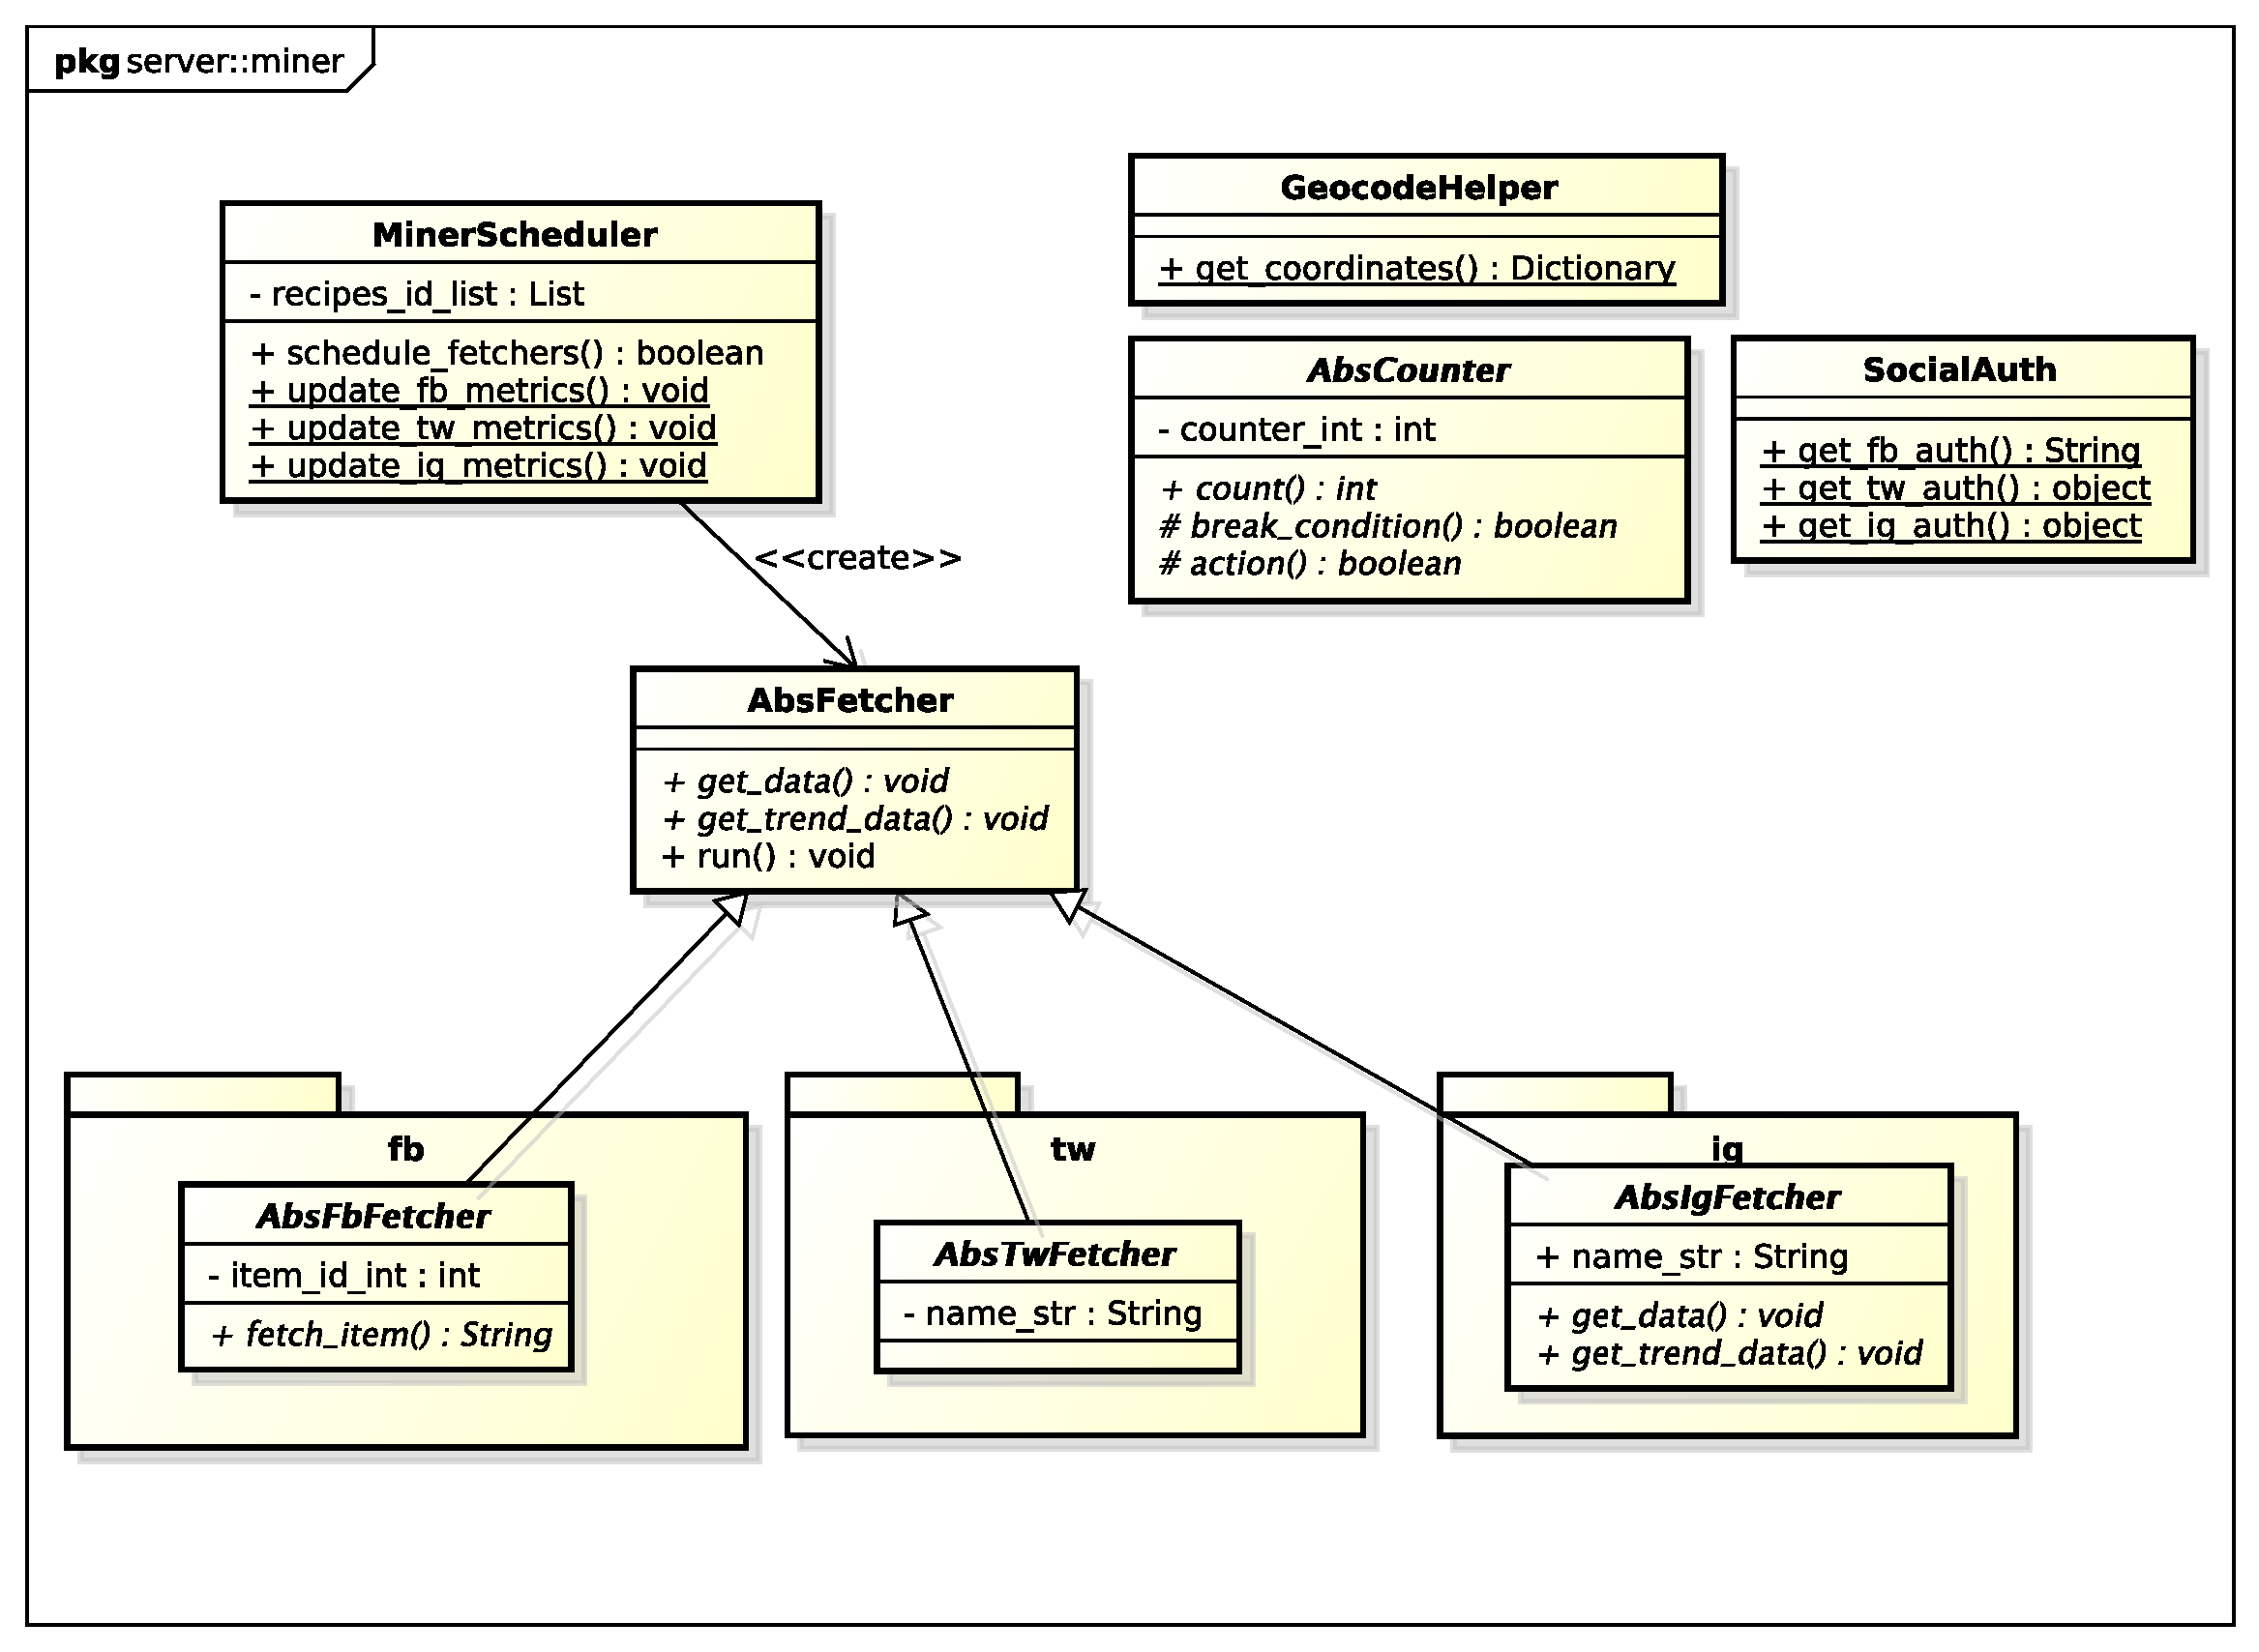
\includegraphics[scale=0.4]{./images/server/miner.pdf}}
	\caption{Package - server::miner}
\end{figure}

\begin{itemize}
  \item \textbf{Descrizione}: è il package che contiene tutte le classi che includono i metodi per prelevare i dati grezzi dai vari social network e salvarli nel database;
  \item \textbf{Padre}: server
  \item \textbf{Package contenuti}:
  	\begin{itemize}
  		\item server::miner::fb
  		\item server::miner::ig
  		\item server::miner::tw
  	\end{itemize}
  \item \textbf{Interazione con altri componenti}:
  	\begin{itemize}
  		\item server::processor
  		\item server::db
  	\end{itemize}
\end{itemize}

\paragraph{Classi} % (fold)
		\subparagraph{server::miner::MinerScheduler} % (fold)
		\label{subp:server_miner_MinerScheduler}
			\begin{itemize}
				\item \textbf{Descrizione}: classe che si occupa di creare i fetcher che preleveranno i dati per ogni metrica di ogni social network;
				\item \textbf{Utilizzo}: contiene la lista degli id delle Recipe da aggiornare ed un metodo che inizializza e avvia i vari fetcher;
				\item \textbf{Relazioni con altre classi}:
					\begin{itemize}
						\item server::miner::AbsFetcher
					\end{itemize}
				\item \textbf{Attributi}:
					\begin{itemize}
						\item recipes\_id\_list : List
					\end{itemize}
				\item \textbf{Metodi}:   
					\begin{itemize}
						\item public schedule\_fetchers() : boolean
					\end{itemize}
			\end{itemize}
		% subparagraph server_miner_MinerScheduler [end]

		\subparagraph{server::miner::AbsCounter} % (fold)
		\label{subp:server_miner_AbsCounter}
			\begin{itemize}
				\item \textbf{Descrizione}: classe astratta che rappresenta il padre delle classi counter delle varie metriche;
				\item \textbf{Utilizzo}: descrive lo scheletro dell'algoritmo di counting necessario ad effettuare il conteggio di determinati dati ricavati con lo scopo ottenere un trend;
				\item \textbf{Relazioni con altre classi}:
					\begin{itemize}
						\item server::miner::fb::AbsFbCounter
						\item server::miner::tw::AbsTwCounter
						\item server::miner::ig::AbsIgCounter
					\end{itemize}
				\item \textbf{Attributi}: 
					\begin{itemize}
						\item counter\_int : int
					\end{itemize}
				\item \textbf{Metodi}:   
					\begin{itemize}
						\item count() : int
						\item break\_condition() : boolean
						\item action() : boolean
					\end{itemize}
			\end{itemize}
		% subparagraph server_miner_AbsCounter [end]

		\subparagraph{server::miner::AbsFetcher} % (fold)
		\label{subp:server_miner_AbsFetcher}
				\begin{itemize}
				\item \textbf{Descrizione}: classe astratta che rappresenta il padre delle classi fetcher dei vari social network;
				\item \textbf{Utilizzo}: è utilizzata per mantenere l'estensibilità nel caso l'applicazione venga estesa con altre API  oltre a quelli dei social network presi in considerazione;
				\item \textbf{Relazioni con altre classi}:
					\begin{itemize}
						\item server::miner::fb::AbsFbFetcher
						\item server::miner::tw::AbsTwFetcher
						\item server::miner::ig::AbsIgFetcher
					\end{itemize}
				\item \textbf{Attributi}: N/A
				\item \textbf{Metodi}: N/A
			\end{itemize}
		% subparagraph server_miner_AbsFetcher [end]

\subsubsection{server::miner::fb} % (fold)
\label{ssub:bdsm_app_server_miner_fb}
\begin{figure}[htbp]
	\centering
	\centerline{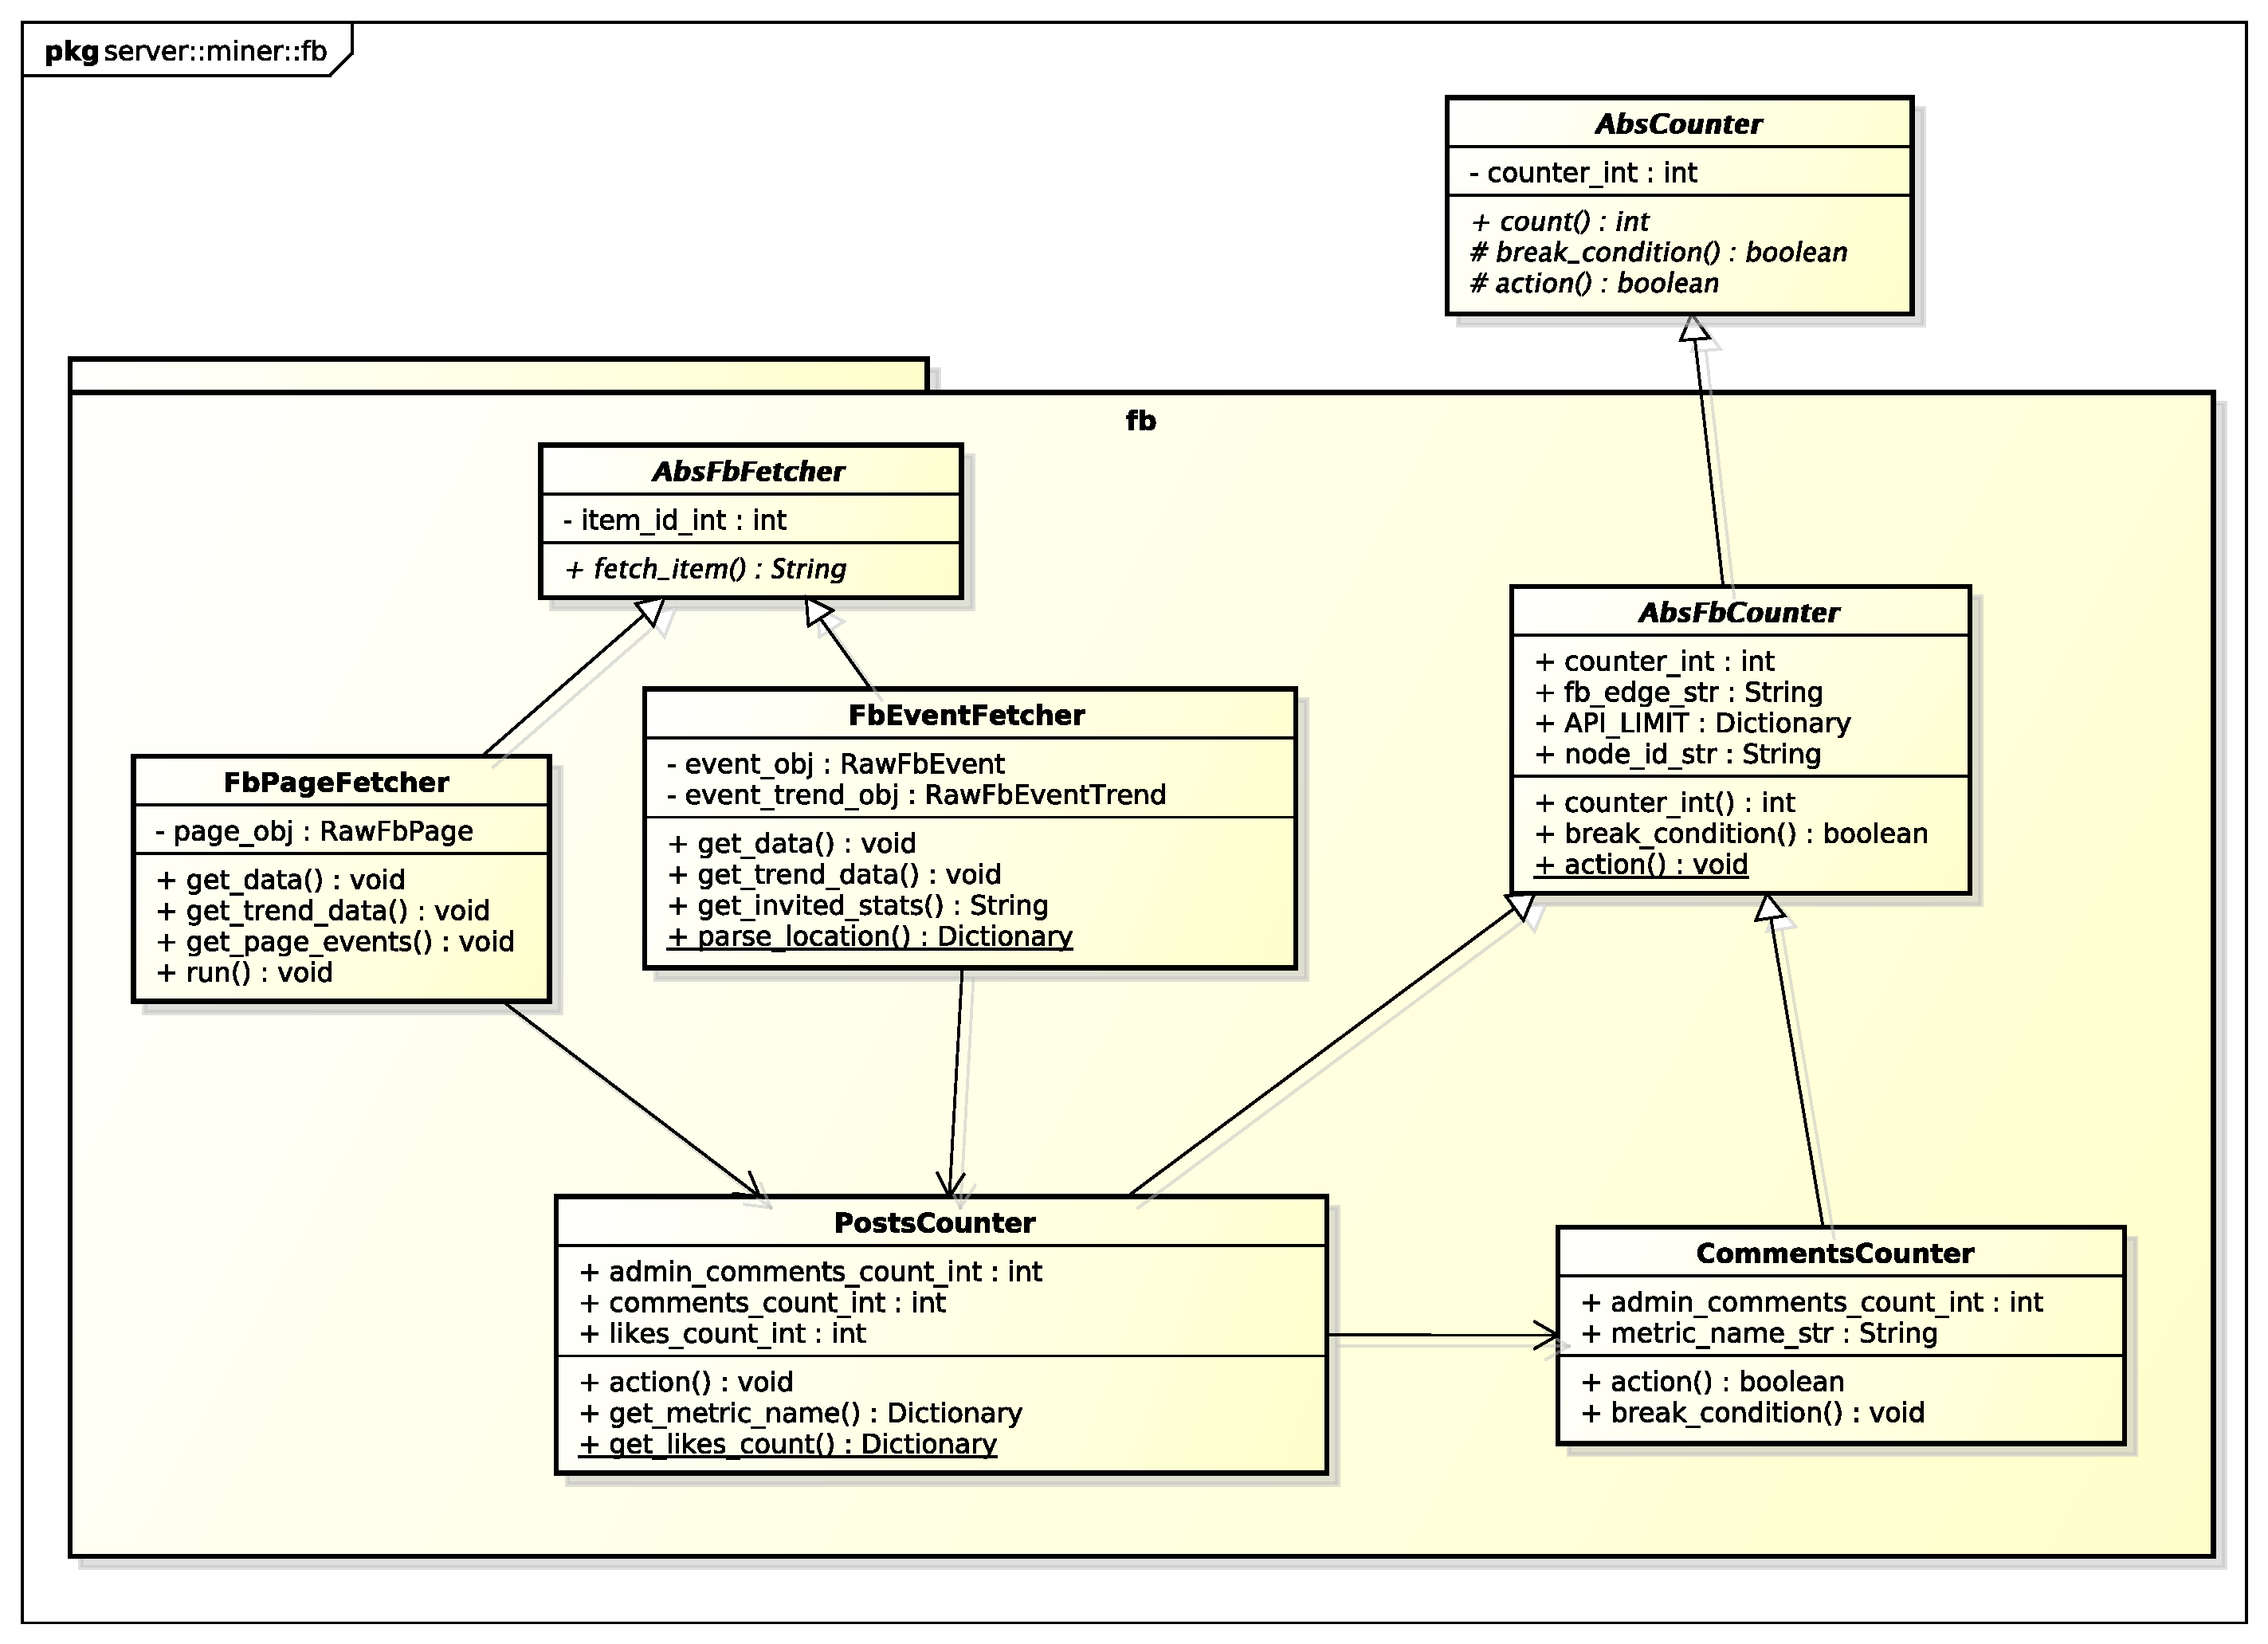
\includegraphics[scale=0.3]{./images/server/miner_fb.pdf}}
	\caption{Package - server::miner::fb}
\end{figure}

\begin{itemize}
  \item \textbf{Descrizione}: è il package che contiene tutte le classi che includono i metodi per prelevare i dati da Facebook e salvarli nel database;
  \item \textbf{Padre}: server::miner
  \item \textbf{Interazione con altri componenti}:
  	\begin{itemize}
  		\item server::db
  	\end{itemize}
\end{itemize}

	\paragraph{Classi} % (fold)
		\subparagraph{server::miner::fb::AbsFbFetcher} % (fold)
		\label{subp:server_miner_fb_AbsFbFetcher}
			\begin{itemize}
				\item \textbf{Descrizione}: classe astratta che rappresenta il padre di ogni fetcher relativo a Facebook;
				\item \textbf{Utilizzo}: contiene un metodo che ricava i dati statici di un'entità Facebook ed un metodo astratto che verrà definito nelle classi figlie;
				\item \textbf{Classi ereditate}: server::miner::AbsFetcher
				\item \textbf{Relazioni con altre classi}:
					\begin{itemize}
						\item server::miner::fb::FbPageFetcher
						\item server::miner::fb::FbEventFetcher
					\end{itemize}
				\item \textbf{Attributi}: 
					\begin{itemize}
						\item item\_id\_str : String
					\end{itemize}
				\item \textbf{Metodi}:   
					\begin{itemize}
						\item public get\_static\_data() : String
						\item get\_trend\_data() : void
					\end{itemize}
			\end{itemize}
	% subparagraph server_miner_fb_AbsFbFetcher [end]

		\subparagraph{server::miner::fb::FbPageFetcher} % (fold)
		\label{subp:server_miner_fb_FbPageFetcher}
			\begin{itemize}
				\item \textbf{Descrizione}: classe che si occupa ricava i dati dalle pagine Facebook;
				\item \textbf{Utilizzo}: contiene un campo che descrive i dati statici di una pagina, un campo che descrive i dati dinamici ed un metodo che li ricava tramite l'utilizzo della classe \texttt{PostsCounter};
				\item \textbf{Classi ereditate}: server::miner::fb::AbsFbFetcher
				\item \textbf{Relazioni con altre classi}:
					\begin{itemize}
						\item server::miner::fb::PostsCounter
					\end{itemize}
				\item \textbf{Attributi}: 
					\begin{itemize}
						\item page\_obj : RawFbPage
						\item page\_trend\_obj : RawFbPageTrend
					\end{itemize}
				\item \textbf{Metodi}:   
					\begin{itemize}
						\item get\_data() : void
						\item get\_trend\_data() : void
					\end{itemize}
			\end{itemize}
		% subparagraph server_miner_fb_FbPageFetcher [end]

		\subparagraph{server::miner::fb::FbEventFetcher} % (fold)
		\label{subp:server_miner_fb_FbEventFetcher}
			\begin{itemize}
				\item \textbf{Descrizione}: classe che ricava i dati di un evento Facebook;
				\item \textbf{Utilizzo}: contiene un campo che descrive i dati statici di un evento, un campo che descrive i dati dinamici e un metodo che li ricava tramite l'utilizzo della classe \texttt{PostsCounter};
				\item \textbf{Classi ereditate}: server::miner::fb::AbsFbFetcher
				\item \textbf{Relazioni con altre classi}:
					\begin{itemize}
						\item server::miner::fb::PostsCounter
					\end{itemize}
				\item \textbf{Attributi}: 
					\begin{itemize}
						\item parent\_key\_int : int
						\item event\_obj : RawFbEvent
					\end{itemize}
				\item \textbf{Metodi}:   
					\begin{itemize}
						\item get\_invited\_stats() : Dictionary
						\item get\_data() : void
						\item get\_trend\_data() : void
					\end{itemize}
			\end{itemize}
	% subparagraph server_miner_fb_FbEventFetcher [end]

		\subparagraph{server::miner::fb::AbsFbCounter} % (fold)
		\label{subp:server_miner_fb_AbsFbCounter}
			\begin{itemize}
				\item \textbf{Descrizione}: classe astratta che rappresenta il padre per tutte le classi counter delle metriche di Facebook;
				\item \textbf{Utilizzo}: classe che contiene l'id delle metriche su cui effettuare il counting, questa classe effettua l'overloading dei metodi della classe padre specificando la struttura dell'algoritmo per il counting su dati Facebook;
				\item \textbf{Classi ereditate}: server::miner::AbsCounter
				\item \textbf{Relazioni con altre classi}:
					\begin{itemize}
						\item server::miner::fb::PostsCounter
						\item server::miner::fb::CommentsCounter
					\end{itemize}
				\item \textbf{Attributi}:  
					\begin{itemize}
						\item counter\_int : int
					\end{itemize}
				\item \textbf{Metodi}:   
					\begin{itemize}
						\item public counter\_int() : int
						\item protected break\_condition() : boolean
						\item protected action() : boolean
					\end{itemize}
			\end{itemize}
	% subparagraph server_miner_fb_AbsFbCounter [end]


	\subparagraph{server::miner::fb::PostsCounter} % (fold)
		\label{subp:server_miner_fb_PostsCounter}
			\begin{itemize}
				\item \textbf{Descrizione}: classe che descrive l'algoritmo per calcolare il numero dei post per ogni evento o pagina;
				\item \textbf{Utilizzo}: classe che contiene un campo per il numero dei like e un campo per il numero dei talking about per ogni post di Facebook;
				\item \textbf{Classe ereditate}: server::miner::fb::AbsFbCounter
				\item \textbf{Relazioni con altre classi}:
					\begin{itemize}
						\item server::miner::fb::CommentsCounter
					\end{itemize}
				\item \textbf{Attributi}:  
					\begin{itemize}
						\item admin\_comments\_count\_int : int
						\item comments\_count\_int : int
						\item likes\_count\_int : int
					\end{itemize}
				\item \textbf{Metodi}:  
					\begin{itemize}
						\item get\_likes\_count(post\_id : String) : int
						\item protected action() : boolean
					\end{itemize}
			\end{itemize}
		% subparagraph server_miner_fb_PostsCounter

	\subparagraph{server::miner::fb::CommentsCounter} % (fold)
		\label{subp:server_miner_fb_CommentsCounter}
			\begin{itemize}
				\item \textbf{Descrizione}: classe che descrive l'algoritmo per calcolare il numero di commenti per ogni post;
				\item \textbf{Utilizzo}: classe che ricava il numero di commenti per ogni post;
				\item \textbf{Classe ereditate}: server::miner::fb::AbsFbCounter
				\item \textbf{Attributi}: 
					\begin{itemize}
						\item metric\_name\_str() : String
					\end{itemize}
				\item \textbf{Metodi}:  
					\begin{itemize}
						\item get\_metric\_name\_str() : String
						\item protected action() : boolean
					\end{itemize}
			\end{itemize}
	% subparagraph server_miner_fb_CommentsCounter


\subsubsection{server::miner::tw} % (fold)
\label{ssub:bdsm_app_server_miner_tw}

\begin{itemize}
  \item \textbf{Descrizione}: è il package che contiene tutte le classi che includono i metodi per prelevare i dati da Twitter e salvarli nel database;
  \item \textbf{Padre}: server::miner
  \item \textbf{Interazione con altri componenti}:
  	\begin{itemize}
  		\item server::db
  	\end{itemize}
\end{itemize}

	\begin{figure}[!htbp]
		\centering
		\centerline{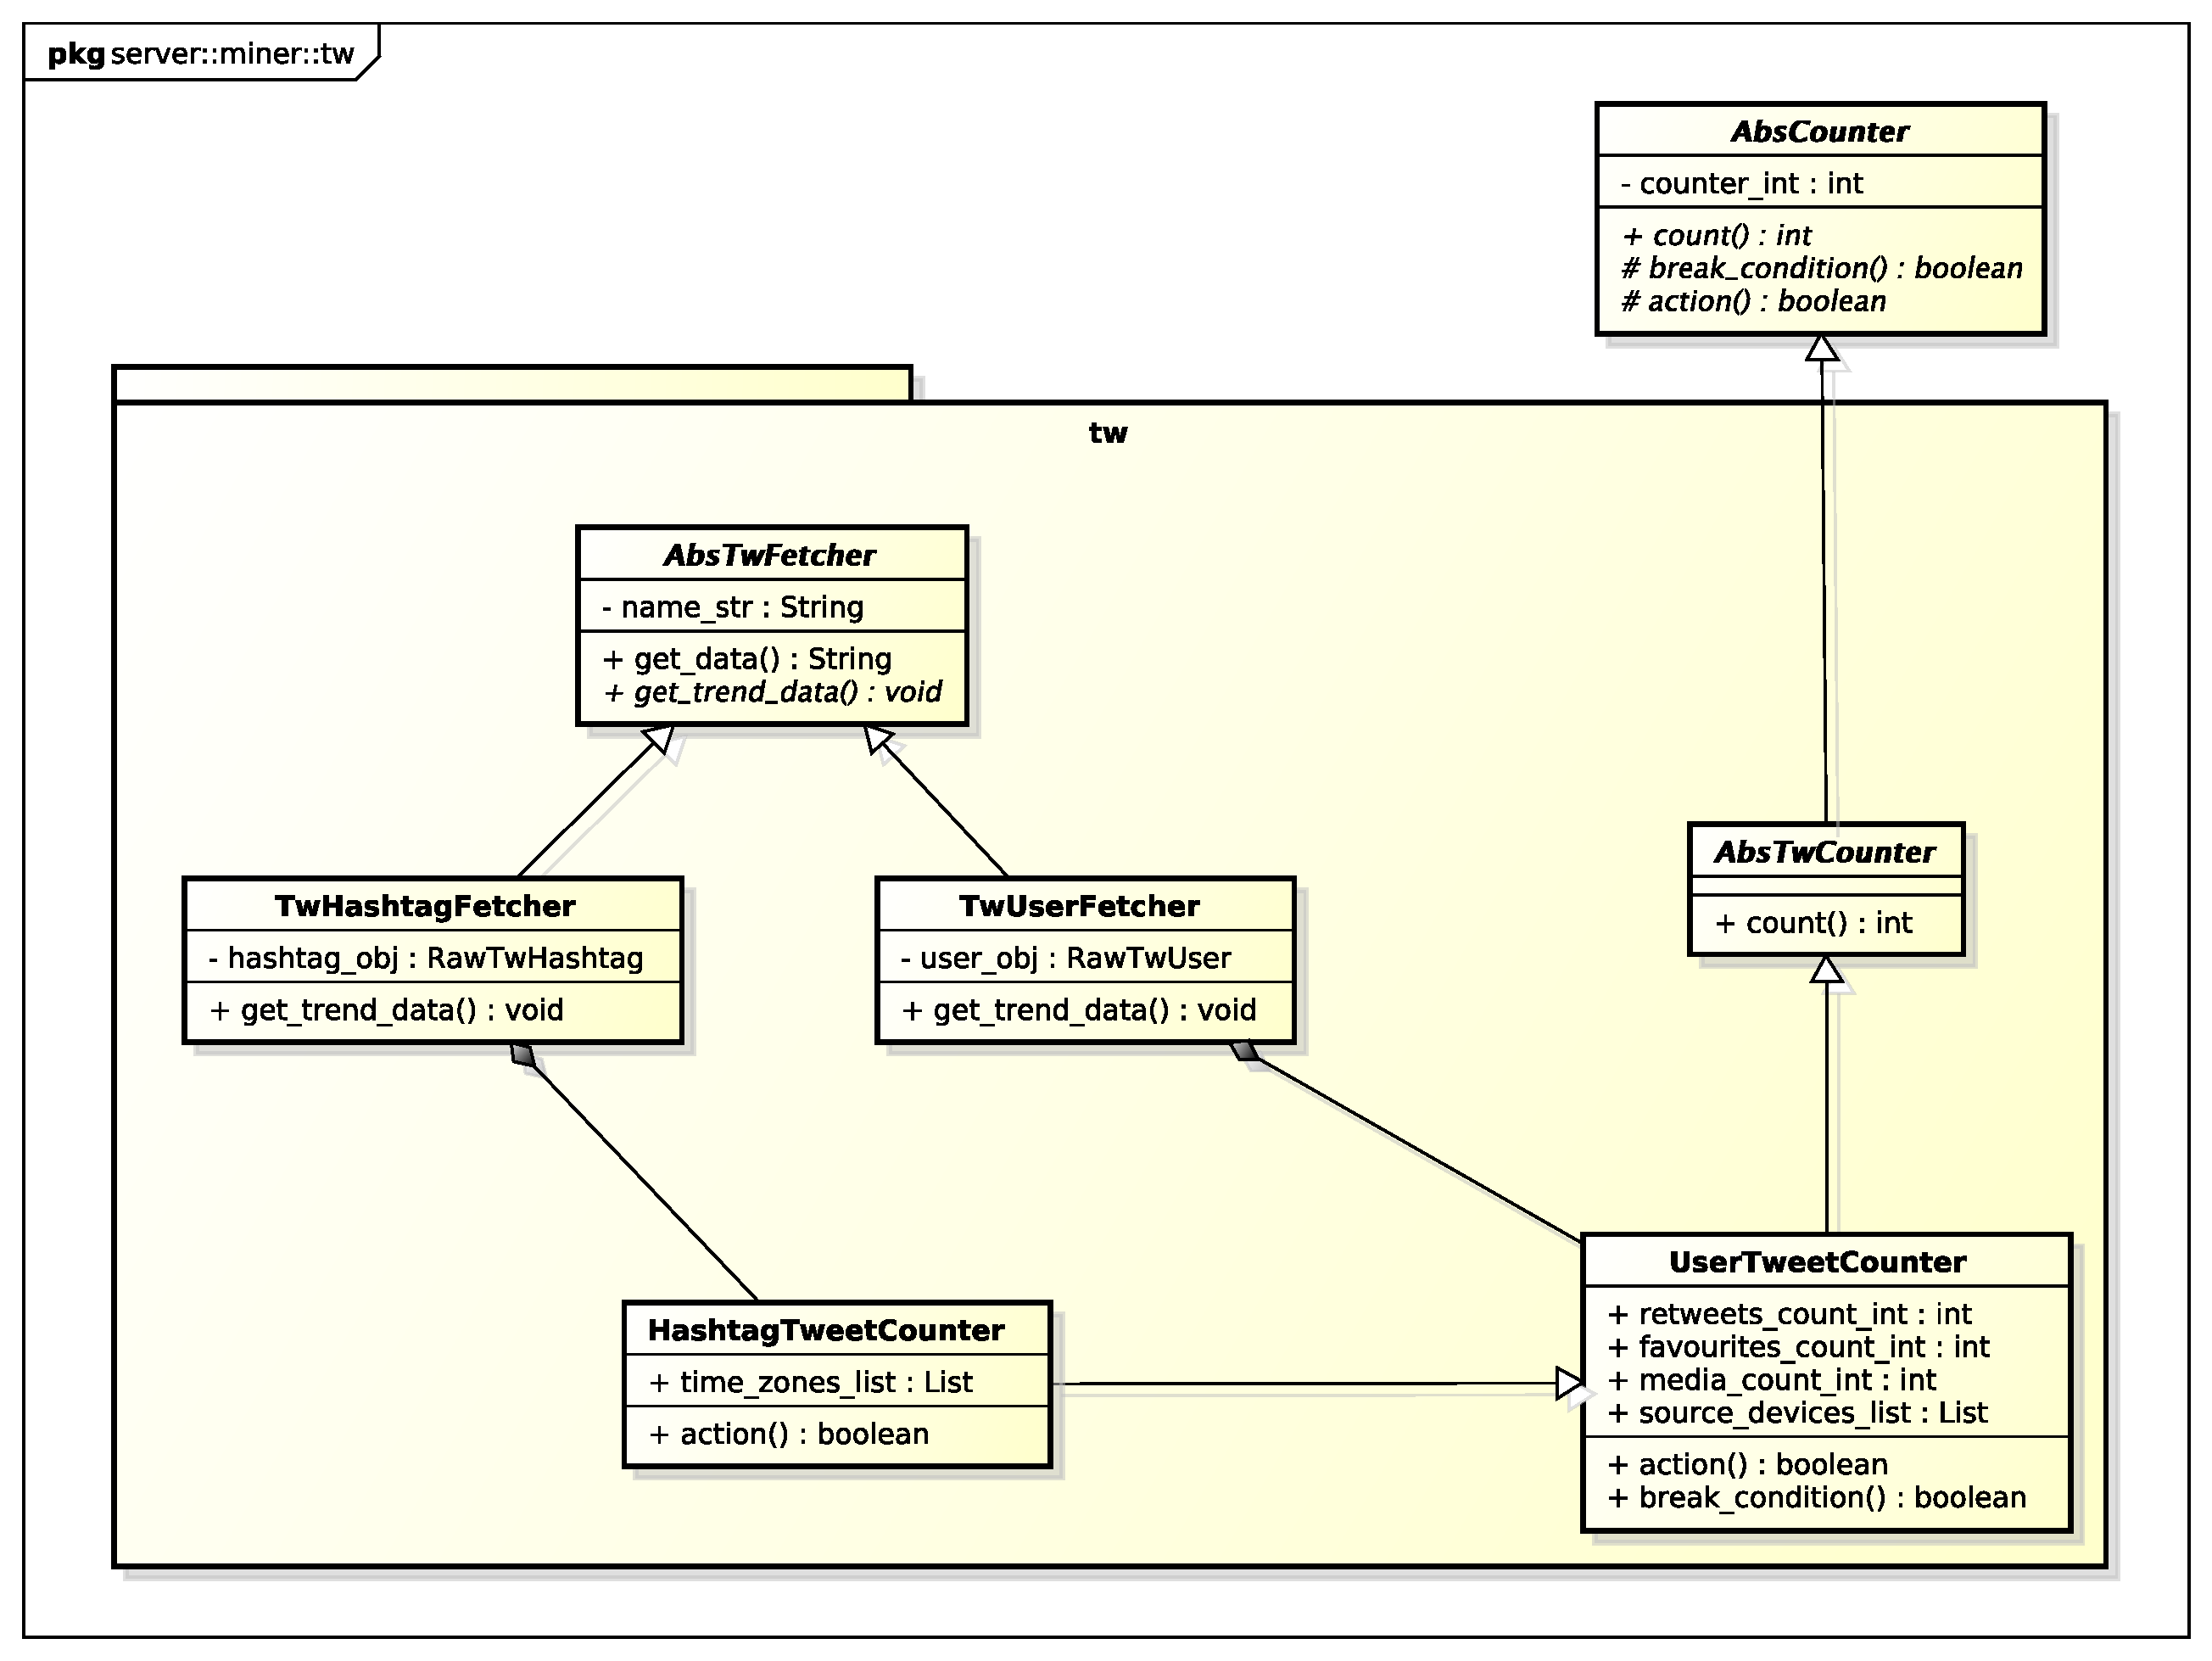
\includegraphics[scale=0.4]{./images/server/miner_tw.pdf}}
		\caption{Package - server::miner::tw}
	\end{figure}

	\paragraph{Classi} % (fold)
	\subparagraph{server::miner::tw::AbsTwFetcher} % (fold)
		\label{subp:server_miner_tw_AbsTwFetcher}
			\begin{itemize}
				\item \textbf{Descrizione}: classe astratta che rappresenta il padre di ogni fetcher relativo a Twitter;
				\item \textbf{Utilizzo}: contiene un metodo che ricava i dati statici di un'entità Twitter ed un metodo astratto che verrà definito nelle classi figlie;
				\item \textbf{Classi ereditate}: server::miner::AbsFetcher
				\item \textbf{Relazioni con altre classi}:
					\begin{itemize}
						\item server::miner::tw::TwHashtagFetcher
						\item server::miner::tw::TwUserFetcher
					\end{itemize}
				\item \textbf{Attributi}:   
					\begin{itemize}
						\item name\_str : String
					\end{itemize}
				\item \textbf{Metodi}:  
					\begin{itemize}
						\item public get\_data() : void
						\item public get\_trend\_data() : void
					\end{itemize}
			\end{itemize}
		% subparagraph server_miner_tw_AbsTwFetcher

	\subparagraph{server::miner::tw::TwHashtagFetcher} % (fold)
		\label{subp:server_miner_tw_TwHashtagFetcher}
			\begin{itemize}
				\item \textbf{Descrizione}: classe che ricava i dati degli hashtag di Twitter;
				\item \textbf{Utilizzo}: classe che contiene un campo che descrive i dati statici di un hashtag di Twitter e un metodo che ricava i dati dinamici tramite l'utilizzo di \texttt{HashtagTweetCounter};
				\item \textbf{Classi ereditate}: server::miner::tw::AbsTwFetcher
				\item \textbf{Relazioni con altre classi}:
					\begin{itemize}
						\item server::miner::tw::HashtagTweetCounter
					\end{itemize}
				\item \textbf{Attributi}:    
					\begin{itemize}
						\item hasjtag\_obj : RawTwHashtag
						\item tweets\_count\_int : int
					\end{itemize}
				\item \textbf{Metodi}:  
					\begin{itemize}
						\item public get\_data() : void
						\item public get\_trend\_data() : void
					\end{itemize}
			\end{itemize}
		% subparagraph server_miner_tw_TwHashtagFetcher

	\subparagraph{server::miner::tw::TwUserFetcher} % (fold)
		\label{subp:server_miner_tw_TwUserFetcher}
			\begin{itemize}
				\item \textbf{Descrizione}: classe che ricava i dati degli utenti di Twitter;
				\item \textbf{Utilizzo}: classe che contiene un campo che descrive i dati statici dell'utente ed un metodo che ricava i dati dinamici tramite l'utilizzo di \texttt{UserTweetCounter};
				\item \textbf{Classi ereditate}: server::miner::tw::AbsTwFetcher
				\item \textbf{Relazioni con altre classi}:
					\begin{itemize}
						\item server::miner::tw::UserTweetCounter
					\end{itemize}
				\item \textbf{Attributi}:    
					\begin{itemize}
						\item user\_obj : RawTwUser
					\end{itemize}
				\item \textbf{Metodi}:  
					\begin{itemize}
						\item public get\_data() : void
						\item public get\_trend\_data() : void
					\end{itemize}
			\end{itemize}
		% subparagraph server_miner_tw_TwUserFetcher

	\subparagraph{server::miner::tw::AbsTwCounter} % (fold)
		\label{subp:server_miner_tw_AbsTwCounter}
			\begin{itemize}
				\item \textbf{Descrizione}: classe astratta che rappresenta il padre per tutte le classi counter delle metriche di Twitter;
				\item \textbf{Utilizzo}: oltre a contenere l’id delle metriche su cui effettuare il counting, questa classe effettua l'overloading dei metodi della classe padre specificando la struttura dell'algoritmo per il counting su dati Twitter;
				\item \textbf{Classi ereditate}: server::miner::AbsCounter
				\item \textbf{Relazioni con altre classi}:
					\begin{itemize}
						\item server::miner::UserTweetCounter
					\end{itemize}
				\item \textbf{Attributi}: N/A
				\item \textbf{Metodi}: 
					\begin{itemize}
						\item public count() : int
					\end{itemize}
			\end{itemize}
		% subparagraph server_miner_tw_AbsTwCounter

	\subparagraph{server::miner::tw::UserTweetCounter} % (fold)
		\label{subp:server_miner_tw_UserTweetCounter}
			\begin{itemize}
				\item \textbf{Descrizione}: classe che descrive l'algoritmo per il counting dei campi di un tweet, relativo ad un utente, di cui ci interessa fare un trend;
				\item \textbf{Utilizzo}: classe che ricava il numero dei retweets, il numero dei favoriti, il tipo di device, e il numero di media per ogni tweet;
				\item \textbf{Classi ereditate}: server::miner::tw::AbsTwCounter
				\item \textbf{Attributi}:    
					\begin{itemize}
						\item public retweets\_count : int
						\item public favourites\_count : int
						\item public source\_devices\_list : List
					\end{itemize}
				\item \textbf{Metodi}:  
					\begin{itemize}
						\item public action() : boolean
						\item public break\_condition() : boolean
					\end{itemize}
			\end{itemize}
		% subparagraph server_miner_tw_UserTweetCounter


	\subparagraph{server::miner::tw::HashtagTweetCounter} % (fold)
		\label{subp:server_miner_tw_HashtagTweetCounter}
			\begin{itemize}
				\item \textbf{Descrizione}: classe che descrive l'algoritmo per il counting dei campi di un tweet, relativo ad un hashtag, di cui ci interessa fare un trend;
				\item \textbf{Utilizzo}: classe che ricava anche la time zone di ogni tweet;
				\item \textbf{Classi ereditate}: server::miner::tw::UserTweetCounter
				\item \textbf{Attributi}:    
					\begin{itemize}
						\item public time\_zones\_list : List
					\end{itemize}
				\item \textbf{Metodi}:  
					\begin{itemize}
						\item public action() : boolean
					\end{itemize}
			\end{itemize}
		% subparagraph server_miner_tw_HashtagTweetCounter

\subsubsection{server::miner::ig} % (fold)
\label{ssub:bdsm_app_server_miner_ig}
\begin{figure}[htbp]
	\centering
	\centerline{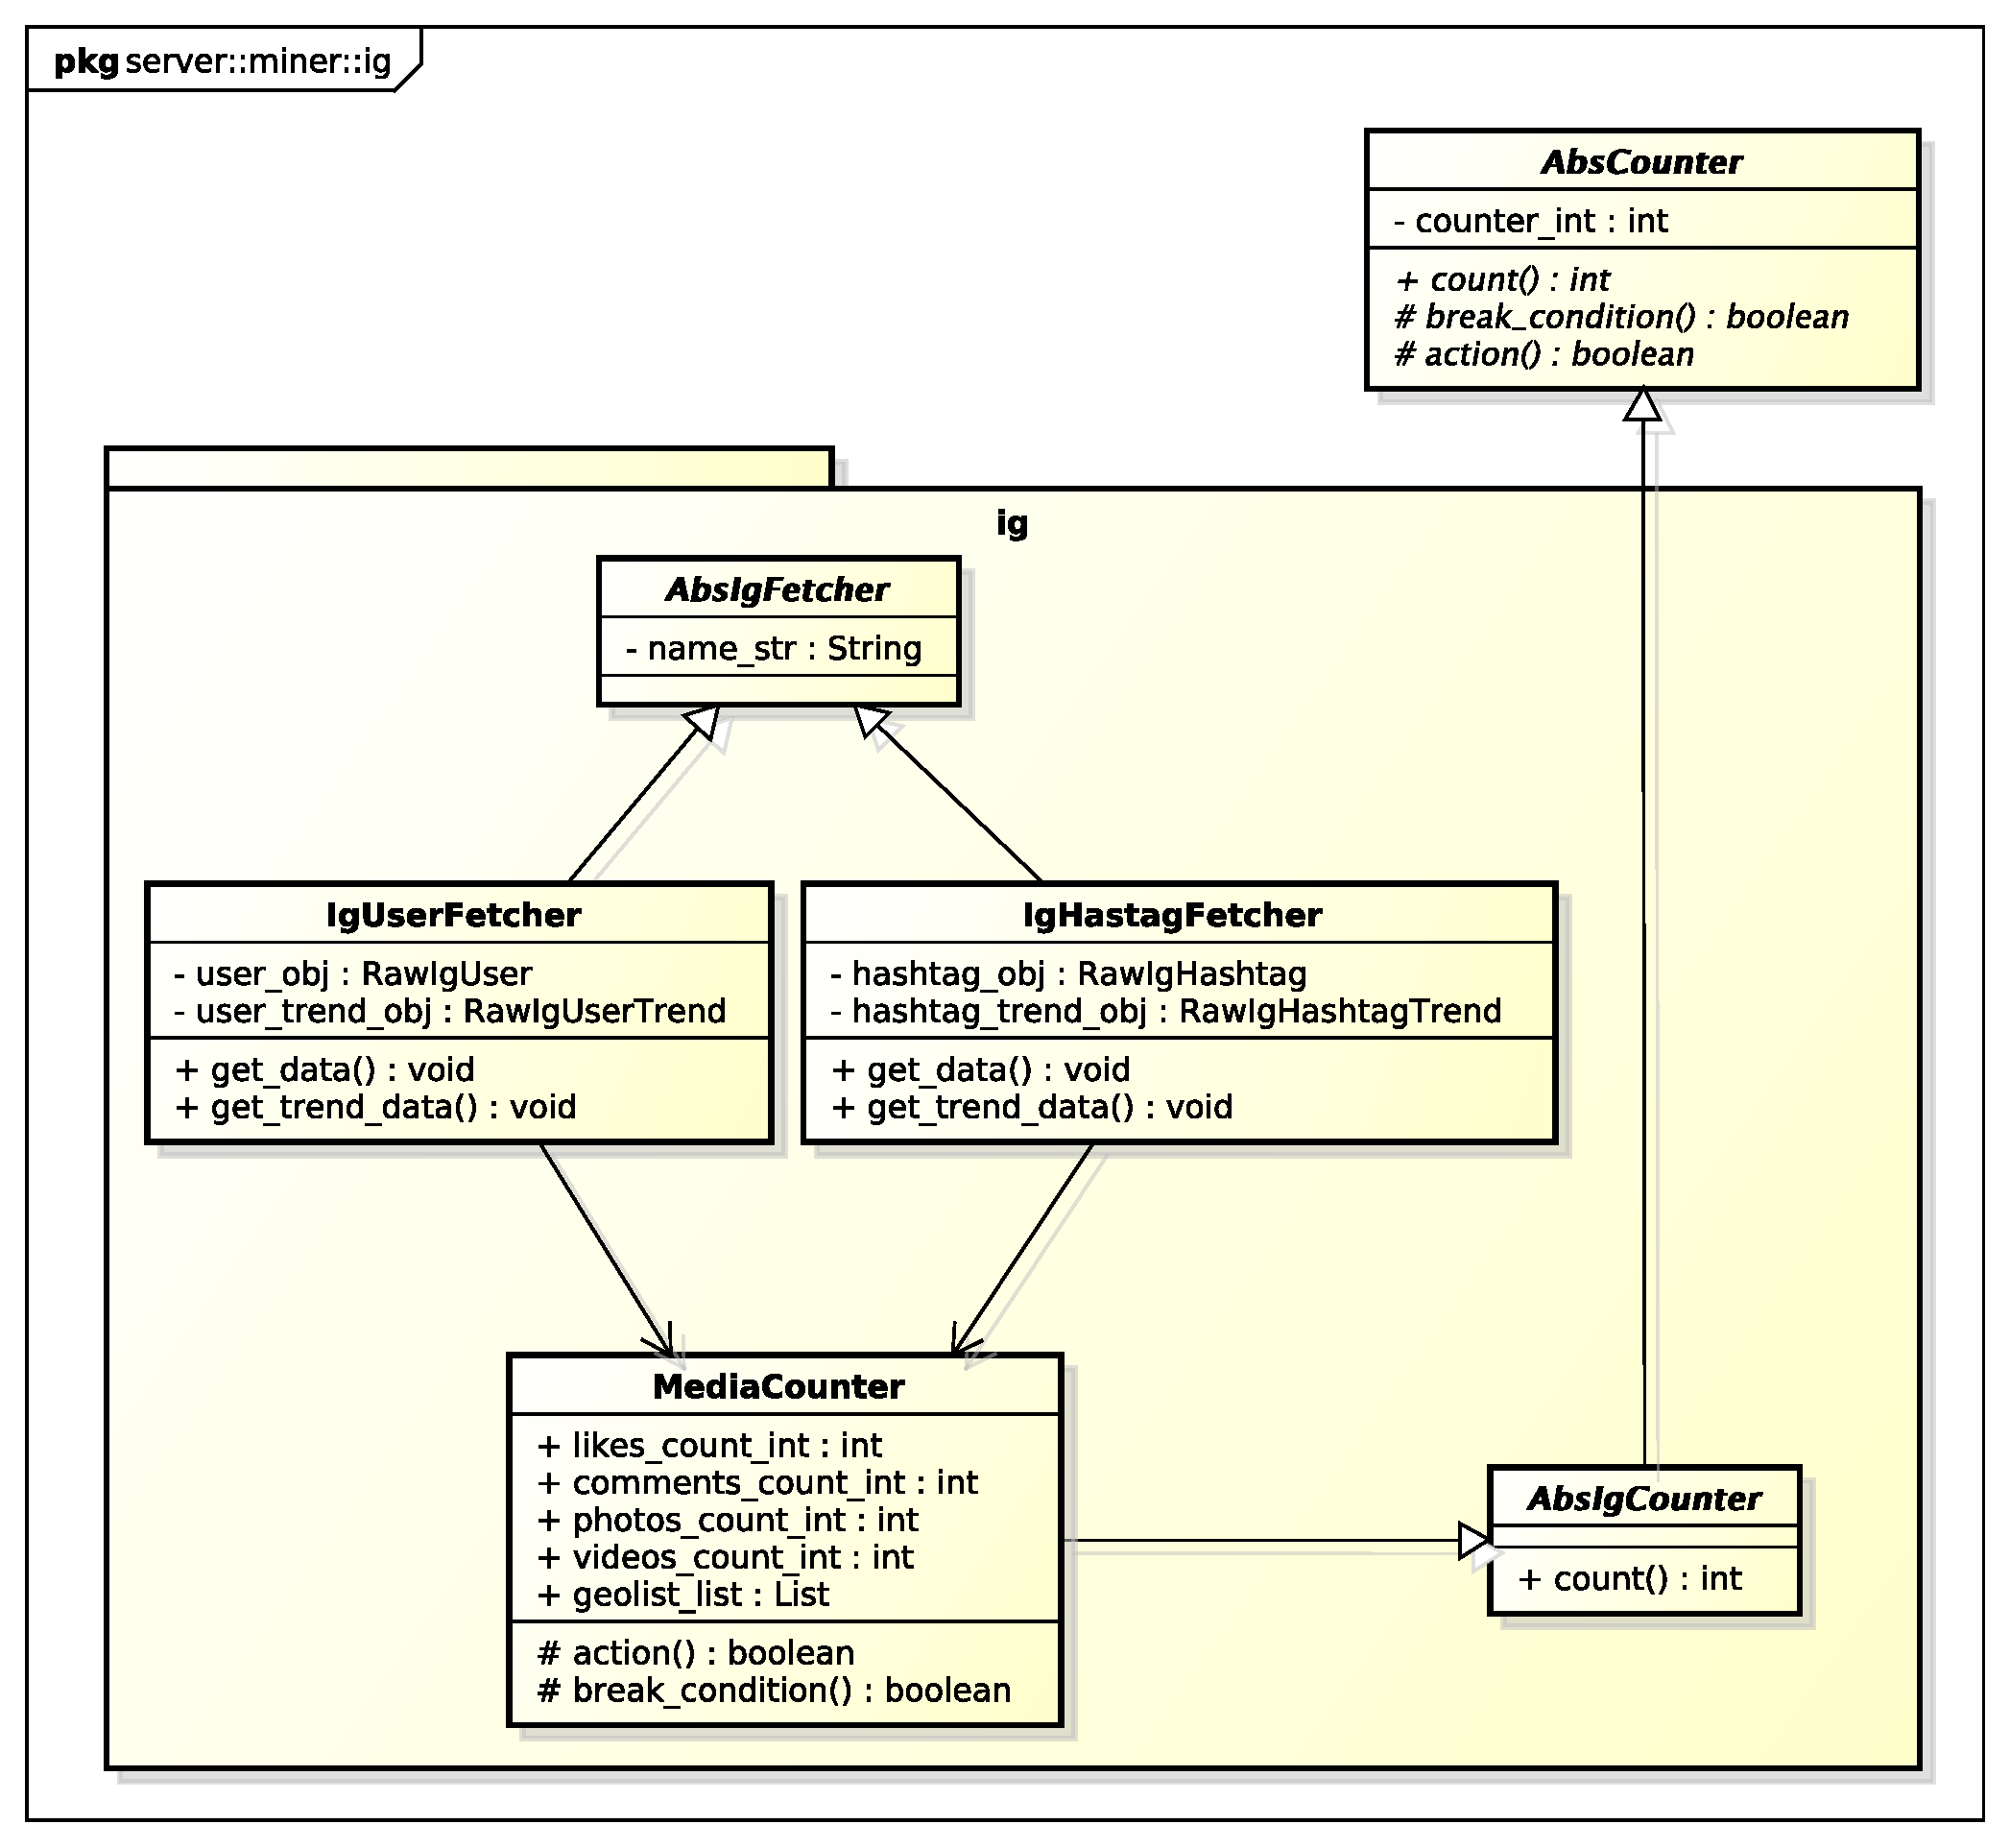
\includegraphics[scale=0.4]{./images/server/miner_ig.pdf}}
	\caption{Package - server::miner::ig}
\end{figure}


\begin{itemize}
  \item \textbf{Descrizione}: è il package che contiene tutte le classi che includono i metodi per prelevare i dati da Instagram e salvarli nel database;
  \item \textbf{Padre}: server::miner
   \item \textbf{Interazione con altri componenti}:
  	\begin{itemize}
  		\item server::db
  	\end{itemize}
\end{itemize}

	\paragraph{Classi} % (fold)
	\subparagraph{server::miner::ig::AbsIgFetcher} % (fold)
		\label{subp:server_miner_ig_AbsIgFetcher}
			\begin{itemize}
				\item \textbf{Descrizione}: classe astratta che rappresenta il padre di ogni fetcher relativo a Instagram;
				\item \textbf{Utilizzo}: contiene un metodo che ricava i dati statici di un'entità Instagram ed un metodo astratto che verrà definito nelle classi figlie;
				\item \textbf{Classi ereditate}: server::miner::AbsFetcher
				\item \textbf{Relazioni con altre classi}:
					\begin{itemize}
						\item server::miner::ig::IgUserFetcher
						\item server::miner::ig::IgHashtagFetcher
					\end{itemize}
				\item \textbf{Attributi}:    
					\begin{itemize}
						\item name\_str : String
					\end{itemize}
				\item \textbf{Metodi}:  
					\begin{itemize}
						\item public get\_data() : void
						\item public get\_trend\_data() : void
					\end{itemize}
			\end{itemize}
		% subparagraph server_miner_ig_AbsIgFetcher

	\subparagraph{server::miner::ig::IgUserFetcher} % (fold)
		\label{subp:server_miner_ig_IgUserFetcher}
			\begin{itemize}
				\item \textbf{Descrizione}: classe che ricava i dati dagli utenti di Instagram;
				\item \textbf{Utilizzo}: classe che contiene un campo che descrive i dati statici dell'utente ed un metodo che ricava i dati dinamici tramite l'utilizzo di \texttt{MediaCounter};
				\item \textbf{Classi ereditate}: server::miner::ig::AbsIgFetcher
				\item \textbf{Relazioni con altre classi}:
					\begin{itemize}
						\item server::miner::ig::MediaCounter
					\end{itemize}
				\item \textbf{Attributi}:    
					\begin{itemize}
						\item user\_obj : RawIgUser
						\item user\_trend\_obj : RawIgUserTrend
					\end{itemize}
				\item \textbf{Metodi}:  
					\begin{itemize}
						\item public get\_data() : void
						\item public get\_trend\_data() : void
					\end{itemize}
			\end{itemize}
		% subparagraph server_miner_ig_IgUserFetcher

	\subparagraph{server::miner::ig::IgHashtagFetcher} % (fold)
		\label{subp:server_miner_ig_IgHashtagFetcher}
			\begin{itemize}
				\item \textbf{Descrizione}: classe che ricava i dati dagli hashtag di Instagram;
				\item \textbf{Utilizzo}: classe che contiene un campo che descrive i dati statici dell'hashtag ed un metodo che ricava i dati dinamici tramite l'utilizzo di \texttt{MediaCounter};
				\item \textbf{Classi ereditate}: server::miner::ig::AbsIgFetcher
				\item \textbf{Relazioni con altre classi}:
					\begin{itemize}
						\item server::miner::ig::MediaCounter
					\end{itemize}
				\item \textbf{Attributi}:    
					\begin{itemize}
						\item hashtag\_obj : RawIgHashtag
						\item hashtag\_trend\_obj : RawIgHashtagTrend
					\end{itemize}
				\item \textbf{Metodi}:  
					\begin{itemize}
						\item public get\_data() : void
						\item public get\_trend\_data() : void
					\end{itemize}
			\end{itemize}
		% subparagraph server_miner_ig_IgHashtagFetcher

	\subparagraph{server::miner::ig::AbsIgCounter} % (fold)
		\label{subp:server_miner_ig_AbsIgCounter}
			\begin{itemize}
				\item \textbf{Descrizione}: classe astratta che rappresenta il padre per tutte le classi counter delle metriche relative ad Instagram;
				\item \textbf{Utilizzo}: classe che contiene l’id delle metriche su cui effettuare il counting, questa classe effettua l'overloading dei metodi della classe padre per specificarne l’utilizzo sui dati relativi ad Instagram;
				\item \textbf{Classi ereditate}: server::miner::AbsCounter
				\item \textbf{Relazioni con altre classi}:
					\begin{itemize}
						\item server::miner::ig::MediaCounter
					\end{itemize}
				\item \textbf{Attributi}: N/A
				\item \textbf{Metodi}: 
					\begin{itemize}
						\item public count() : int
					\end{itemize}
			\end{itemize}
		% subparagraph server_miner_ig_AbsIgCounter


	\subparagraph{server::miner::ig::MediaCounter} % (fold)
		\label{subp:server_miner_ig_MediaCounter}
			\begin{itemize}
				\item \textbf{Descrizione}: classe che descrive l'algoritmo per il counting delle metriche necessarie a descrivere il trend dei media di un utente o di un hashtag  Instagram;
				\item \textbf{Utilizzo}: classe che ricava il numero di commenti, il numero di like, il numero di foto e il numero di video di un media;
				\item \textbf{Classi ereditate}: server::miner::ig::AbsIgCounter
				\item \textbf{Attributi}:    
					\begin{itemize}
						\item public likes\_count\_int : int
						\item public comments\_count\_int : int
						\item public photos\_count\_int : int
						\item public videos\_count\_int : int
						\item public geolist\_list : List
					\end{itemize}
				\item \textbf{Metodi}:  
					\begin{itemize}
						\item protected action() : boolean
						\item protected break\_condition() : boolean
					\end{itemize}
			\end{itemize}
		% subparagraph server_miner_ig_MediaCounter


% subsubsection
 \clearpage \newpage
  % END PACKAGE MINER

  % PACKAGE ENDPOINTS
  % =================================================================================================
% File:			server_tier/endpoints.tex
% Description:	Definisce la sezione relativa al back-end dell'applicazione
% Created:		2015-04-07
% Author:		Cusinato Giacomo
% Email:		cusinato.giacomo@mashup-unipd.it
% =================================================================================================
% Modification History:
% Version		Modifier Date		Change											Author
% 0.0.1
% =================================================================================================

% CONTENUTO DEL CAPITOLO


\subsubsection{server::endpoints} % (fold)
\label{ssub:bdsm_app_server_endpoints}
\begin{figure}[!htbp]
	\centering
	\centerline{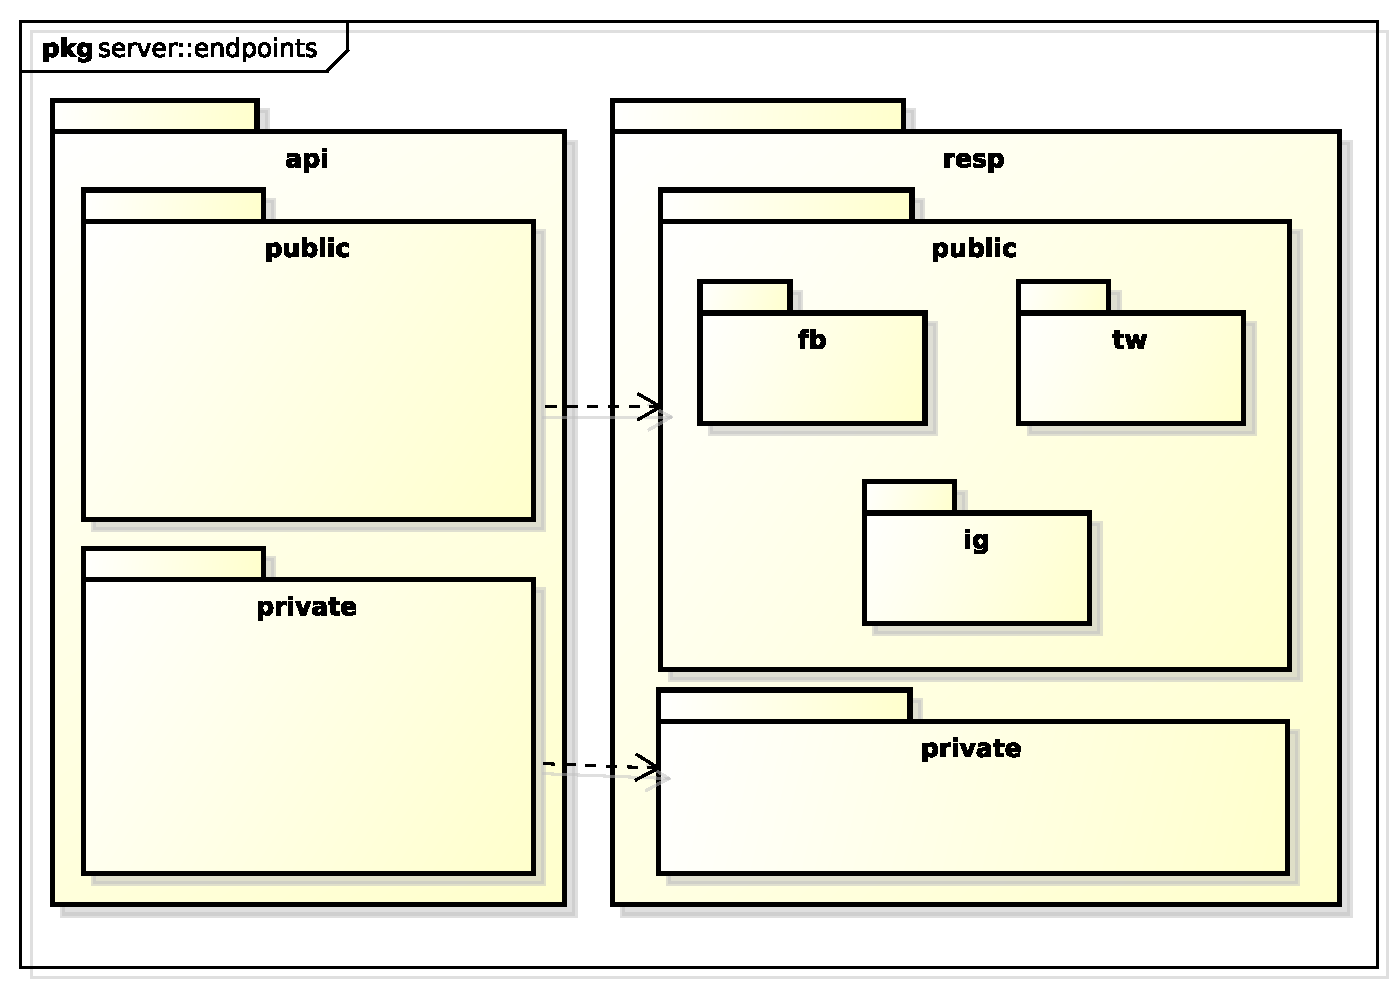
\includegraphics[scale=0.6]{./images/server/endpoints.pdf}}
	\caption{Package - server::endpoints}
\end{figure}

\begin{itemize}
  \item \textbf{Descrizione}: è il package che contiene tutte le classi che implementato l'interfaccia REST del sistema tramite Google Cloud Endpoints;
  \item \textbf{Padre}: server
  \item \textbf{Package contenuti}:
  	\begin{itemize}
  		\item server::endpoints::api
  		\item server::endpoints::resp
	\end{itemize}
  \item \textbf{Interazione con altri componenti}:
  	\begin{itemize}
  		\item server::processor
  		\item server::db
	\end{itemize}
\end{itemize}
% subsubsection

\subsubsection{server::endpoints::api} % (fold)
\label{ssub:bdsm_app_server_endpoints_api}

	In questo package e nei suoi package figli viene utilizzata la classe \textbf{ResourceContainer} offerta dai Google Cloud Endpoints per le richieste contenenti percorsi e query.
\begin{figure}[!htbp]
	\centering
	\centerline{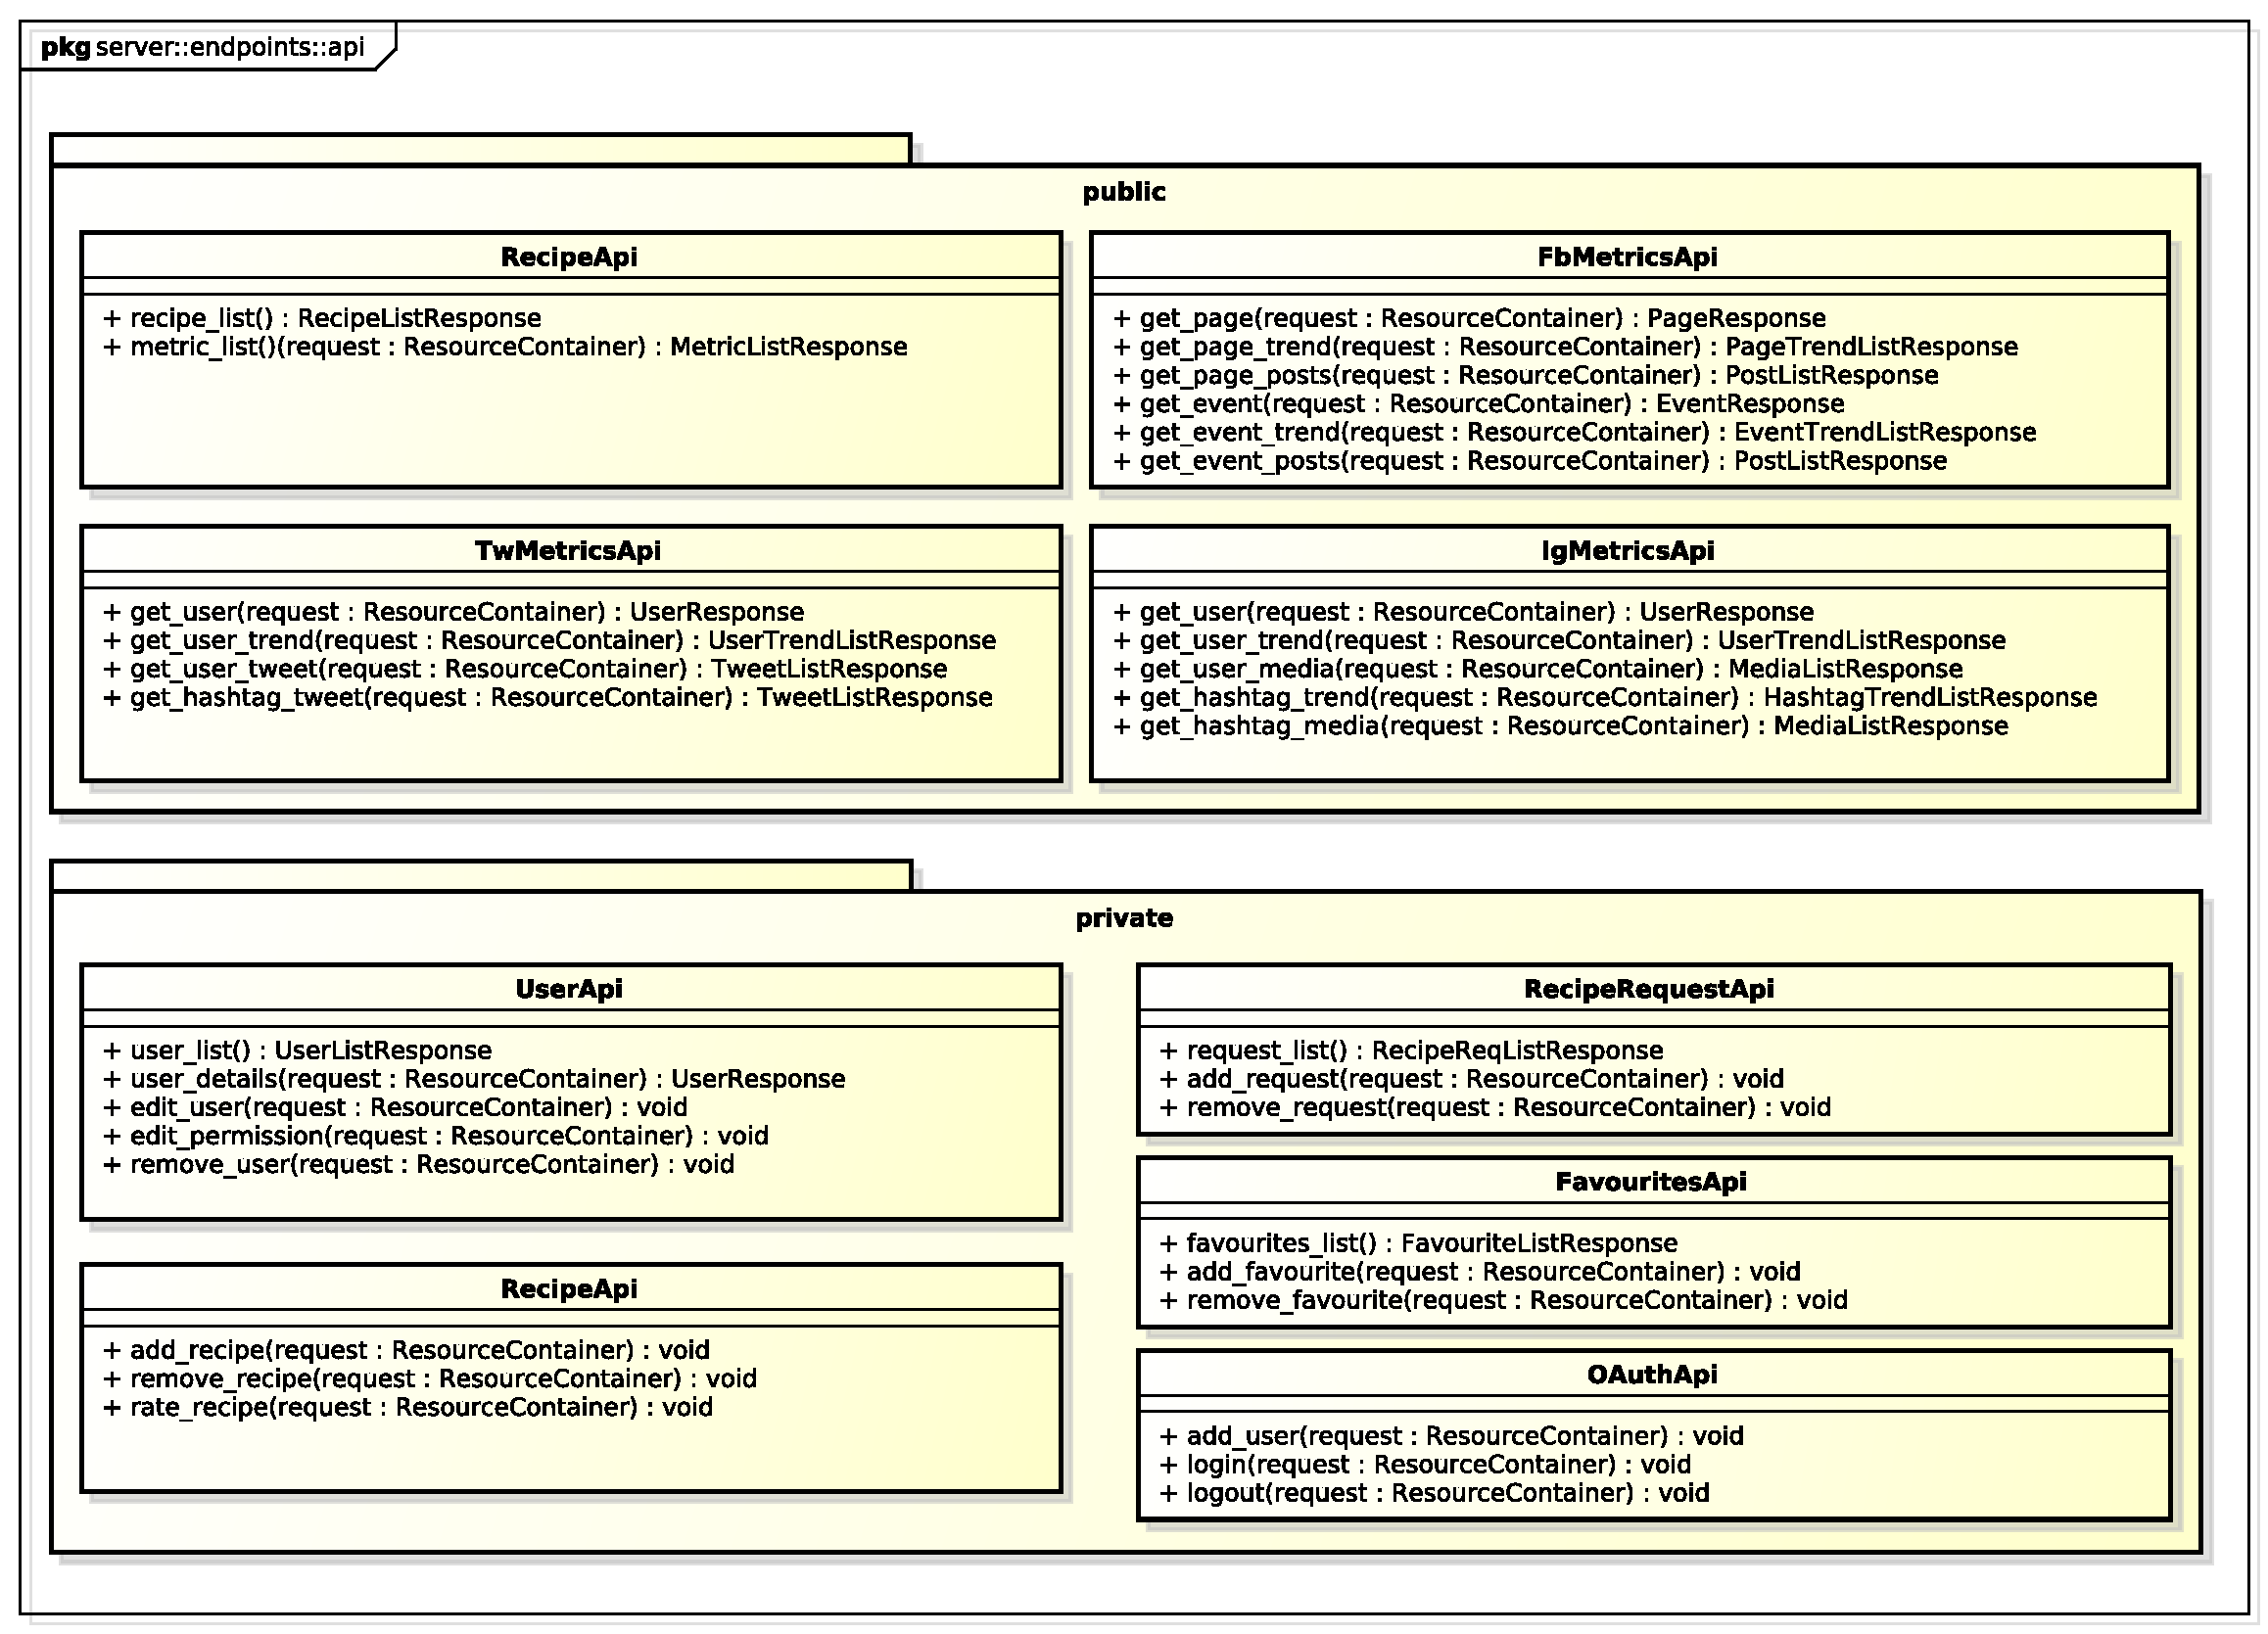
\includegraphics[scale=0.4]{./images/server/api.pdf}}
	\caption{Package - server::endpoints::api}
\end{figure}

\begin{itemize}
  \item \textbf{Descrizione}: è il package che definisce le web API offerte dall'applicazione e utilizzati dal client;
  \item \textbf{Padre}: server::endpoints
  \item \textbf{Package contenuti}:
  	\begin{itemize}
  		\item server::endpoints::api::public
  		\item server::endpoints::api::private
	\end{itemize}
  \item \textbf{Interazione con altri componenti}:
  	\begin{itemize}
  		\item client::model::services
  		\item server::processor
  		\item server::db
			\item server::endpoints::resp
	\end{itemize}
\end{itemize}
% subsubsection

\subsubsection{server::endpoints::api::public} % (fold)
\label{ssub:bdsm_app_server_endpoints_api_public}
\begin{figure}[!htbp]
	\centering
	\centerline{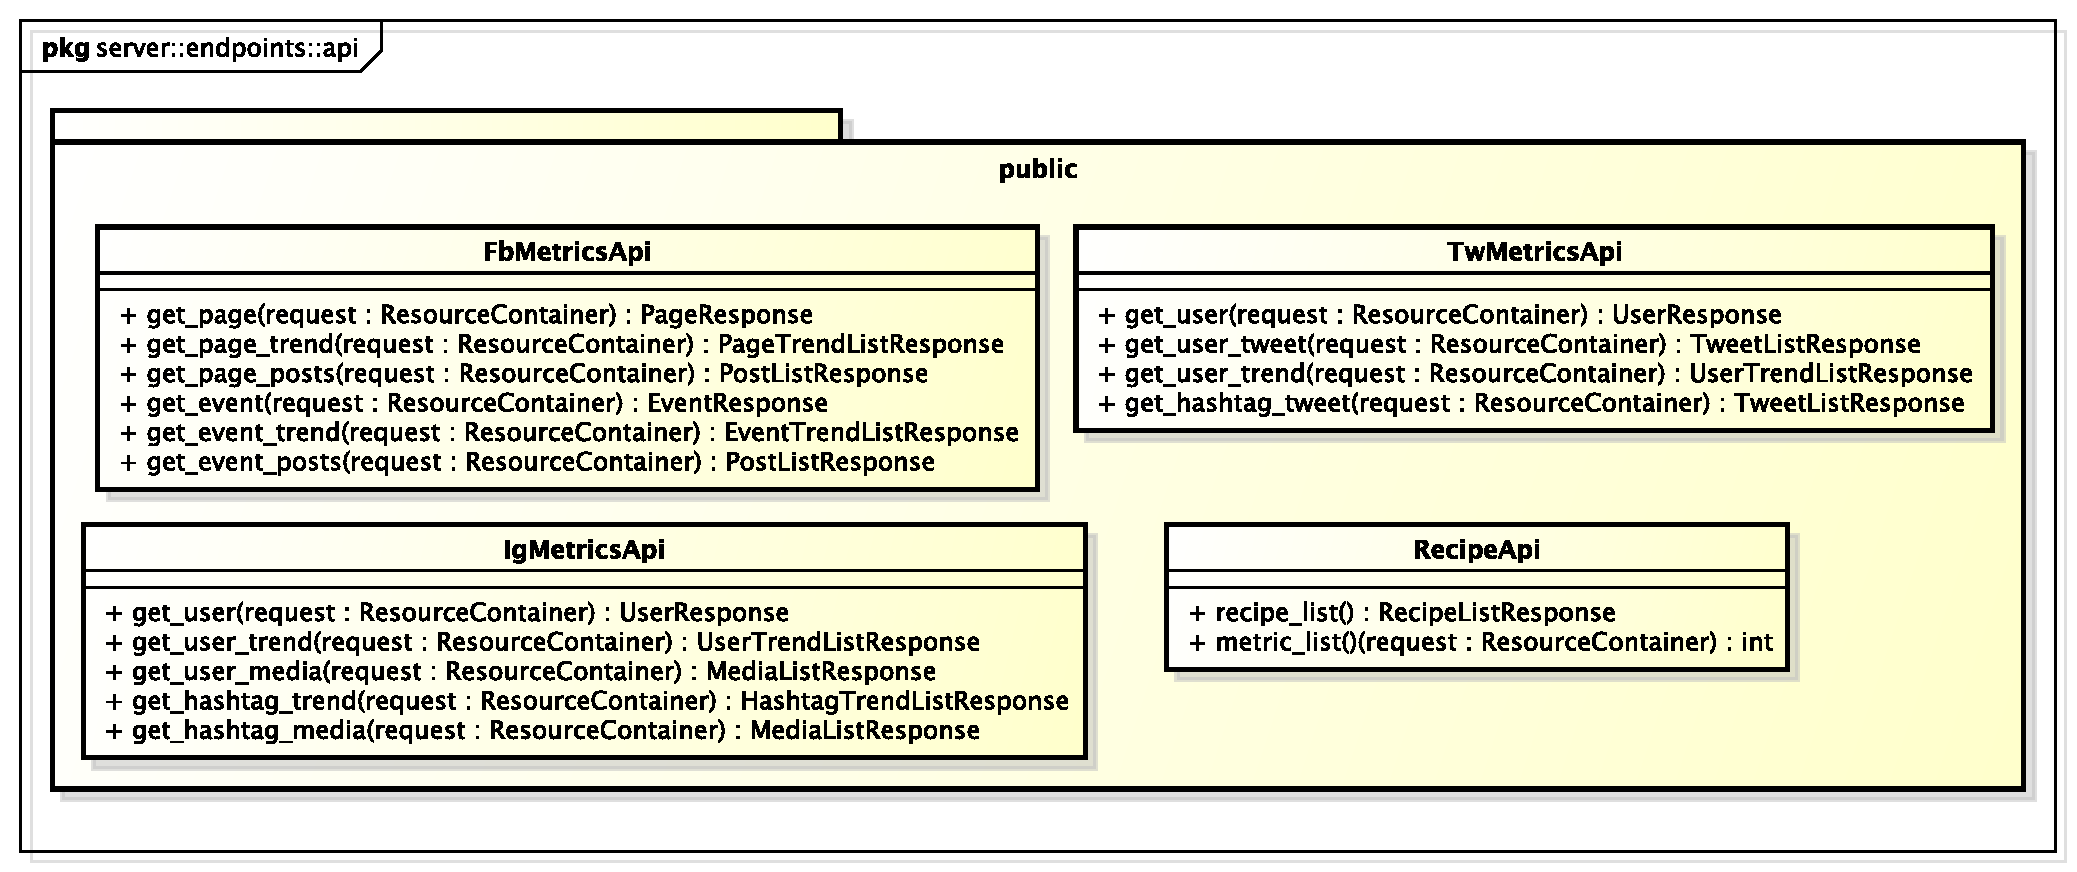
\includegraphics[scale=0.4]{./images/server/api_public.pdf}}
	\caption{Package - server::endpoints::api::public}
\end{figure}

\begin{itemize}
  \item \textbf{Descrizione}: è il package contenente l'implementazione delle web API pubbliche;
  \item \textbf{Padre}: server::endpoints::api
  \item \textbf{Interazione con altri componenti}:
  	\begin{itemize}
        \item server::processor
				\item server::endpoints::resp::public
    \end{itemize}
\end{itemize}
% subsubsection

	\paragraph{Classi} % (fold)

    \subparagraph{server::endpoints::api::public::RecipeApi} % (fold)
    \label{subp:bdsm_app_server_endpoints_api_public_recipeapi}
    \begin{itemize}
      \item \textbf{Descrizione}: classe utilizzata in seguito ad una chiamata del client per ricavare la lista delle Recipe e delle metriche;
      \item \textbf{Utilizzo}: i suoi metodi vengono invocati quando viene richiesto dal client di recuperare la lista delle Recipe e delle metriche;
      \item \textbf{Relazioni con altre classi}:
        \begin{itemize}
          \item server::endpoints::resp::public::MetricListResponse;
          \item server::endpoints::resp::private::RecipeListResponse;
        \end{itemize}
		\item \textbf{Attributi}: TO DO
		\item \textbf{Metodi}: TO DO
      \end{itemize}
    % subparagraph bdsm_app_server_endpoints_api_public_recipeapi (end)

    \subparagraph{server::endpoints::api::public::FbMetricsApi} % (fold)
    \label{subp:bdsm_app_server_endpoints_api_public_fbmetricsapi}
    \begin{itemize}
      \item \textbf{Descrizione}: classe utilizzata in seguito ad una chiamata del client per ottenere i dati relativi ad una metrica di Facebook;
      \item \textbf{Utilizzo}: i suoi metodi vengono invocati quando viene richiesto dal client dei dati relativi ad una pagina o ad un evento di Facebook;
      \item \textbf{Relazioni con altre classi}:
        \begin{itemize}
          \item server::endpoints::resp::public::fb::PageResponse
          \item server::endpoints::resp::public::fb::PageTrendListResponse
          \item server::endpoints::resp::public::fb::PostListResponse
          \item server::endpoints::resp::public::fb::EventResponse
          \item server::endpoints::resp::public::fb::EventTrendListResponse
        \end{itemize}
		\item \textbf{Attributi}: TO DO
		\item \textbf{Metodi}: TO DO
      \end{itemize}
    % subparagraph bdsm_app_server_endpoints_api_public_fbmetricsapi (end)

    \subparagraph{server::endpoints::api::public::TwMetricsApi} % (fold)
    \label{subp:bdsm_app_server_endpoints_api_public_twmetricsapi}
    \begin{itemize}
      \item \textbf{Descrizione}: classe utilizzata in seguito ad una chiamata del client per ottenere i dati relativi ad una metrica di Twitter;
      \item \textbf{Utilizzo}: i suoi metodi vengono invocati quando viene richiesto dal client dei dati relativi ad un utente o un hashtag di Twitter;
      \item \textbf{Relazioni con altre classi}:
        \begin{itemize}
          \item server::endpoints::resp::public::tw::UserResponse
          \item server::endpoints::resp::public::tw::UserTrendListResponse
          \item server::endpoints::resp::public::tw::TweetListResponse
        \end{itemize}
		\item \textbf{Attributi}: TO DO
		\item \textbf{Metodi}: TO DO
      \end{itemize}
    % subparagraph bdsm_app_server_endpoints_api_public_twmetricsapi (end)

    \subparagraph{server::endpoints::api::public::IgMetricsApi} % (fold)
    \label{subp:bdsm_app_server_endpoints_api_public_igmetricsapi}
    \begin{itemize}
      \item \textbf{Descrizione}: classe utilizzata in seguito ad una chiamata del client per ottenere i dati relativi ad una metrica di Instagram;
      \item \textbf{Utilizzo}: i suoi metodi vengono invocati quando viene richiesto dal client dei dati relativi ad un utente o hashtag di Instagram;
      \item \textbf{Relazioni con altre classi}:
        \begin{itemize}
          \item server::endpoints::resp::public::ig::UserResponse
          \item server::endpoints::resp::public::ig::UserTrendListResponse
          \item server::endpoints::resp::public::ig::MediaListResponse
          \item server::endpoints::resp::public::ig::HashtagTrendListResponse
        \end{itemize}
		\item \textbf{Attributi}: TO DO
		\item \textbf{Metodi}: TO DO
      \end{itemize}
    % subparagraph bdsm_app_server_endpoints_api_public_igmetricsapi (end)

\subsubsection{server::endpoints::api::private} % (fold)
\label{ssub:bdsm_app_server_endpoints_api_private}
\begin{figure}[!htbp]
	\centering
	\centerline{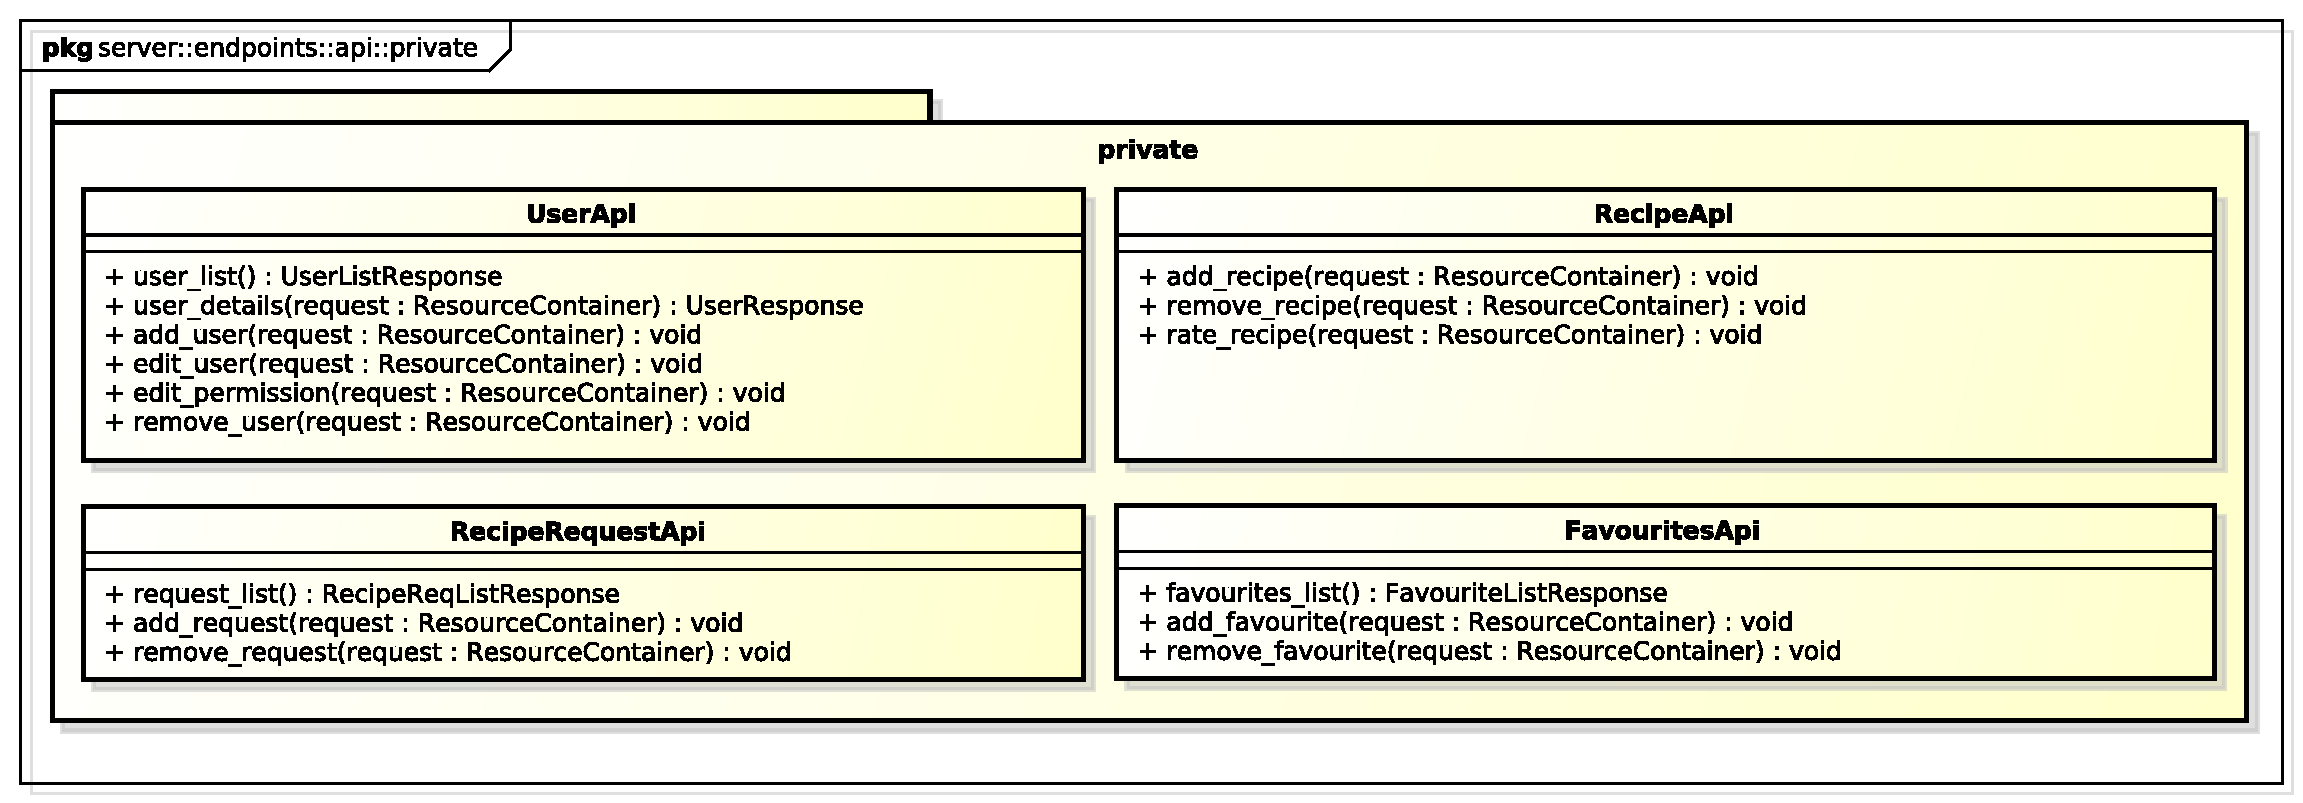
\includegraphics[scale=0.4]{./images/server/api_private.pdf}}
	\caption{Package - server::endpoints::api::private}
\end{figure}

\begin{itemize}
  \item \textbf{Descrizione}: è il package contenente l'implementazione delle web API private;
  \item \textbf{Padre}: server::endpoints::api
  \item \textbf{Interazione con altri componenti}:
  	\begin{itemize}
        \item server::processor
				\item server::endpoints::resp::private
    \end{itemize}
\end{itemize}
% subsubsection

	\paragraph{Classi} % (fold)

    \subparagraph{server::endpoints::api::private::RecipeApi} % (fold)
    \label{subp:bdsm_app_server_endpoints_api_private_recipeapi}
    \begin{itemize}
      \item \textbf{Descrizione}: classe che rappresenta l'implementazione delle web API relative alla gestione delle Recipe;
      \item \textbf{Utilizzo}: i suoi metodi vengono invocati quando viene richiesto dal client di aggiungere, rimuovere o valutare una Recipe;
      \item \textbf{Relazioni con altre classi}:
        \begin{itemize}
          \item server::endpoints::resp::private::RecipeListResponse
        \end{itemize}
		\item \textbf{Attributi}: TO DO
		\item \textbf{Metodi}: TO DO
      \end{itemize}
    % subparagraph bdsm_app_server_endpoints_api_private_recipeapi (end)

    \subparagraph{server::endpoints::api::private::UserApi} % (fold)
    \label{subp:bdsm_app_server_endpoints_api_private_userapi}
    \begin{itemize}
      \item \textbf{Descrizione}: classe che rappresenta l'implementazione delle web API relative alla gestione degli utenti;
      \item \textbf{Utilizzo}: i suoi metodi vengono invocati quando viene richiesto dal client di ricavare la lista degli utenti, di aggiungere o rimuovere un utente, ricavare o modificare i dati di un utente o per modificare i dati di un utente;
      \item \textbf{Relazioni con altre classi}:
        \begin{itemize}
          \item server::endpoints::resp::private::UserResponse
          \item server::endpoints::resp::private::UserListResponse
        \end{itemize}
		\item \textbf{Attributi}: TO DO
		\item \textbf{Metodi}: TO DO
      \end{itemize}
    % subparagraph bdsm_app_server_endpoints_api_private_userapi (end)

    \subparagraph{server::endpoints::api::private::RecipeRequestApi} % (fold)
    \label{subp:bdsm_app_server_endpoints_api_private::reciperequestapi}
    \begin{itemize}
      \item \textbf{Descrizione}: classe che rappresenta l'implementazione delle web API relative alla gestione delle richieste di aggiunta Recipe;
      \item \textbf{Utilizzo}: i suoi metodi vengono invocati quando viene inviata una richiesta di nuova Recipe o la rimozione di una richiesta esistente da parte del client;
      \item \textbf{Relazioni con altre classi}:
        \begin{itemize}
          \item server::endpoints::resp::private::RecipeReqListResponse
        \end{itemize}
		\item \textbf{Attributi}: TO DO
		\item \textbf{Metodi}: TO DO
      \end{itemize}
    % subparagraph bdsm_app_server_endpoints_api_private_reciperequestapi (end)

    \subparagraph{server::endpoints::api::private::FavoritesApi} % (fold)
    \label{subp:bdsm_app_server_endpoints_api_private_favoritesapi}
    \begin{itemize}
      \item \textbf{Descrizione}: classe che rappresenta l'implementazione delle web API relative alla gestione delle View preferite per ogni utente;
      \item \textbf{Utilizzo}: i suoi metodi vengono invocati quando viene richiesto dal client l'inserimento di una View nei preferiti o quando viene richiesta la rimozione di una View aggiunta in precedenza;
      \item \textbf{Relazioni con altre classi}:
        \begin{itemize}
          \item server::endpoints::resp::private::FavoriteListResponse
        \end{itemize}
		\item \textbf{Attributi}: TO DO
		\item \textbf{Metodi}: TO DO
      \end{itemize}
    % subparagraph bdsm_app_server_endpoints_api_private_favoritesapi (end)

\subsubsection{server::endpoints::resp} % (fold)
\label{ssub:bdsm_app_server_endpoints_resp}
\begin{figure}[!htbp]
	\centering
	\centerline{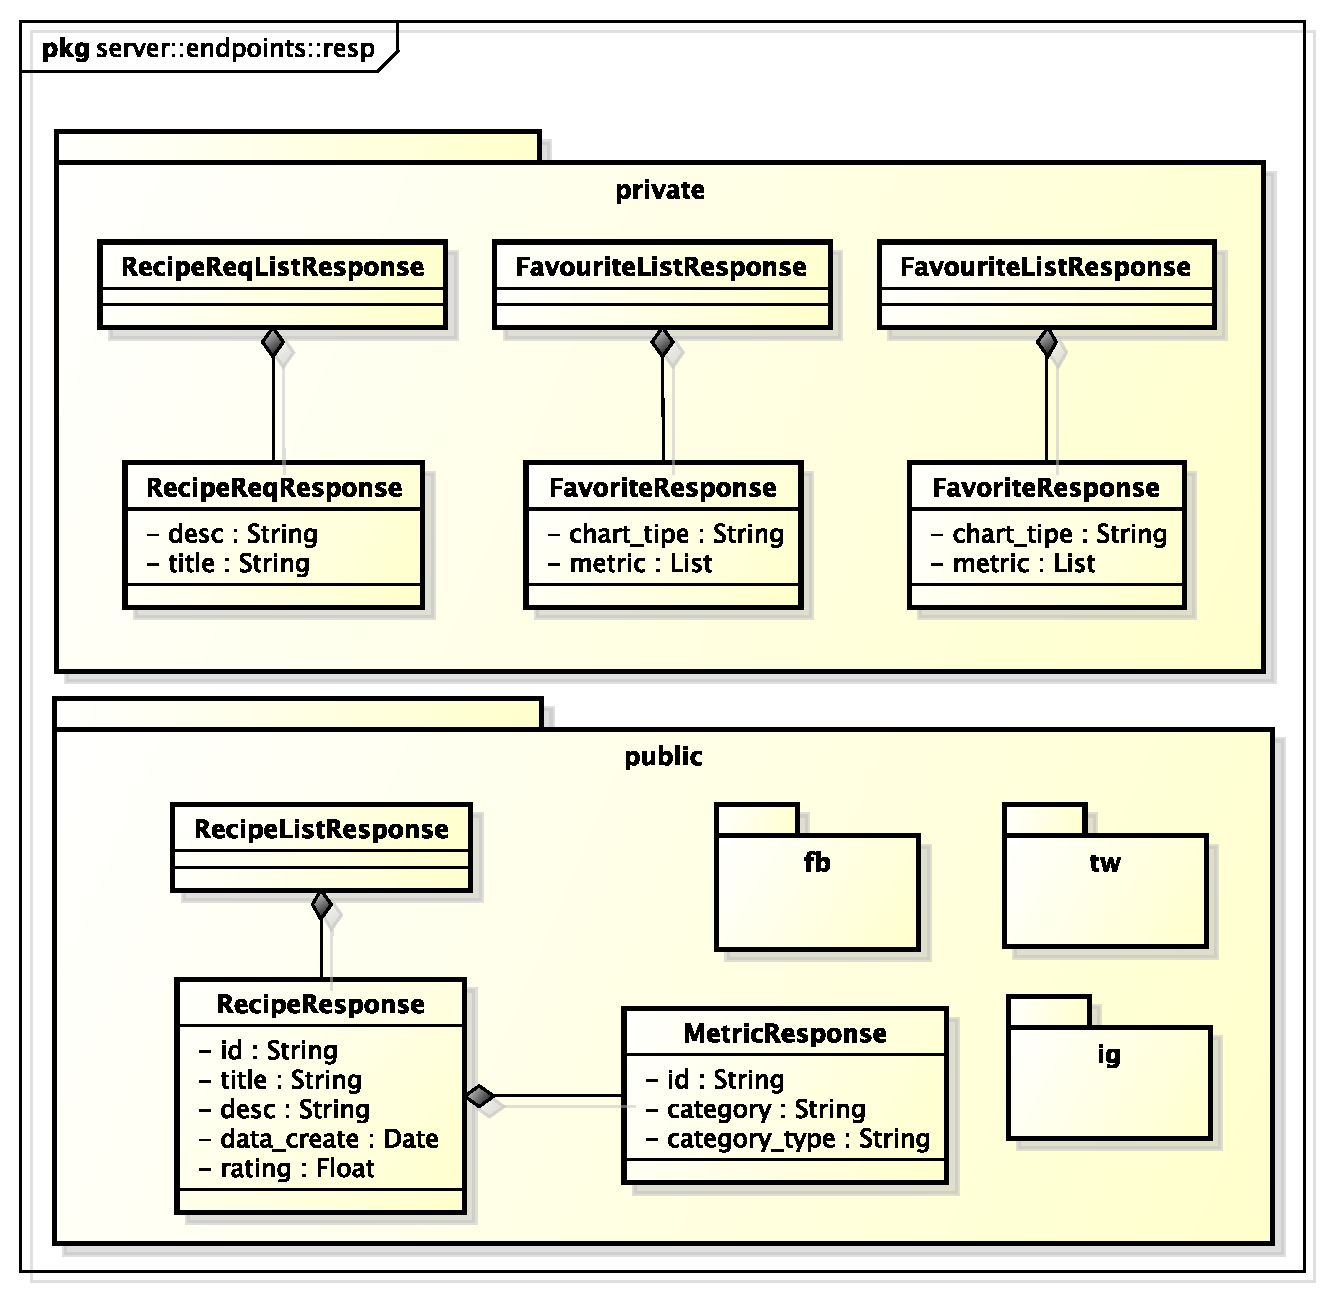
\includegraphics[scale=0.45]{./images/server/resp.pdf}}
	\caption{Package - server::endpoints::resp}
\end{figure}

\begin{itemize}
  \item \textbf{Descrizione}: è il package che definisce il modelli delle risposte da passare al client in seguito alle chiamate API;
  \item \textbf{Padre}: server::endpoints
  \item \textbf{Package contenuti}:
  	\begin{itemize}
  		\item server::endpoints::resp::public
  		\item server::endpoints::resp::private
	\end{itemize}
\end{itemize}
% subsubsection

\subsubsection{server::endpoints::resp::public} % (fold)
\label{ssub:bdsm_app_server_endpoints_resp_public}
\begin{figure}[!htbp]
	\centering
	\centerline{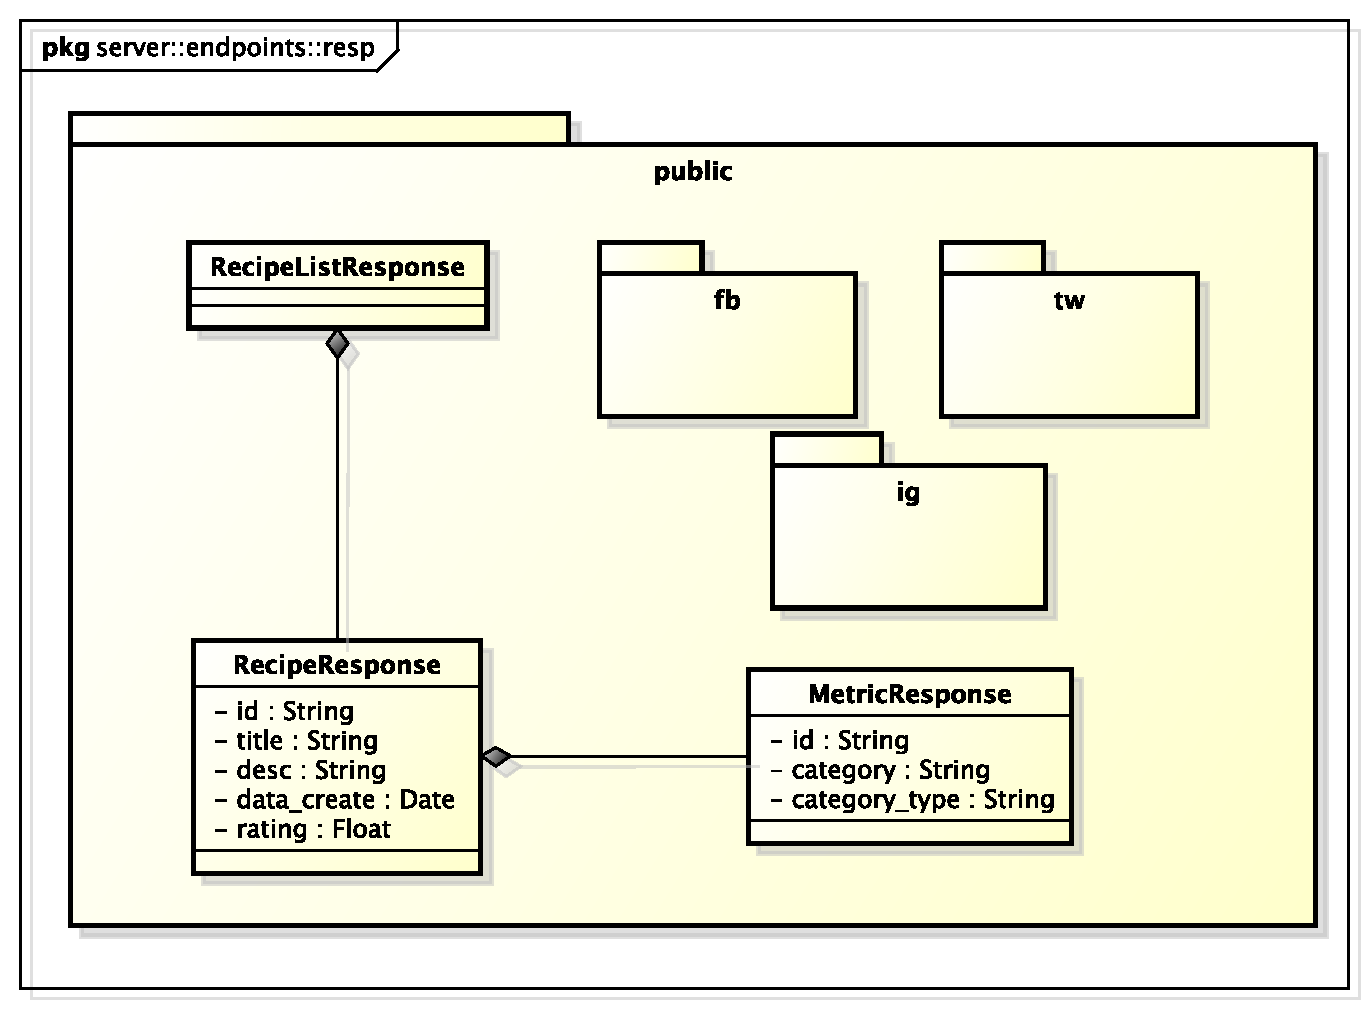
\includegraphics[scale=0.55]{./images/server/resp_public.pdf}}
	\caption{Package - server::endpoints::resp::public}
\end{figure}

\begin{itemize}
  \item \textbf{Descrizione}: è il package che definisce il modello delle risposte da passare al client in seguito alle chiamate delle API pubbliche;
  \item \textbf{Padre}: server::endpoints::resp
  \item \textbf{Package contenuti}:
  	\begin{itemize}
  		\item server::endpoints::resp::public::fb
  		\item server::endpoints::resp::public::tw
  		\item server::endpoints::resp::public::ig
	\end{itemize}
  \item \textbf{Interazione con altri componenti}:
  	\begin{itemize}
  		\item server::endpoints::resp::private
	\end{itemize}
\end{itemize}
% subsubsection

	\paragraph{Classi} % (fold)

    \subparagraph{server::endpoints::resp::public::MetricListResponse} % (fold)
    \label{subp:bdsm_app_server_endpoints_resp_public_metriclistresponse}
    \begin{itemize}
      \item \textbf{Descrizione}: rappresenta il modello dei dati della lista di metriche da ritornare al client;
      \item \textbf{Utilizzo}: viene utilizzata dalle API per restituire la response della lista delle metriche relative ad un Recipe al client;
      \item \textbf{Relazioni con altre classi}:
        \begin{itemize}
          \item server::endpoints::resp::public::fb::PageResponse
          \item server::endpoints::resp::public::fb::EventResponse
          \item server::endpoints::resp::public::tw::UserResponse
          \item server::endpoints::resp::public::tw::HashtagResponse
          \item server::endpoints::resp::public::ig::UserResponse
          \item server::endpoints::resp::public::ig::HashtagResponse
        \end{itemize}
		\item \textbf{Attributi}: TO DO
		\item \textbf{Metodi}: TO DO
      \end{itemize}
    % subparagraph bdsm_app_server_endpoints_resp_public_metriclistresponse (end)

\subsubsection{server::endpoints::resp::public::fb} % (fold)
\label{ssub:bdsm_app_server_endpoints_resp_public_fb}
\begin{figure}[!htbp]
	\centering
	\centerline{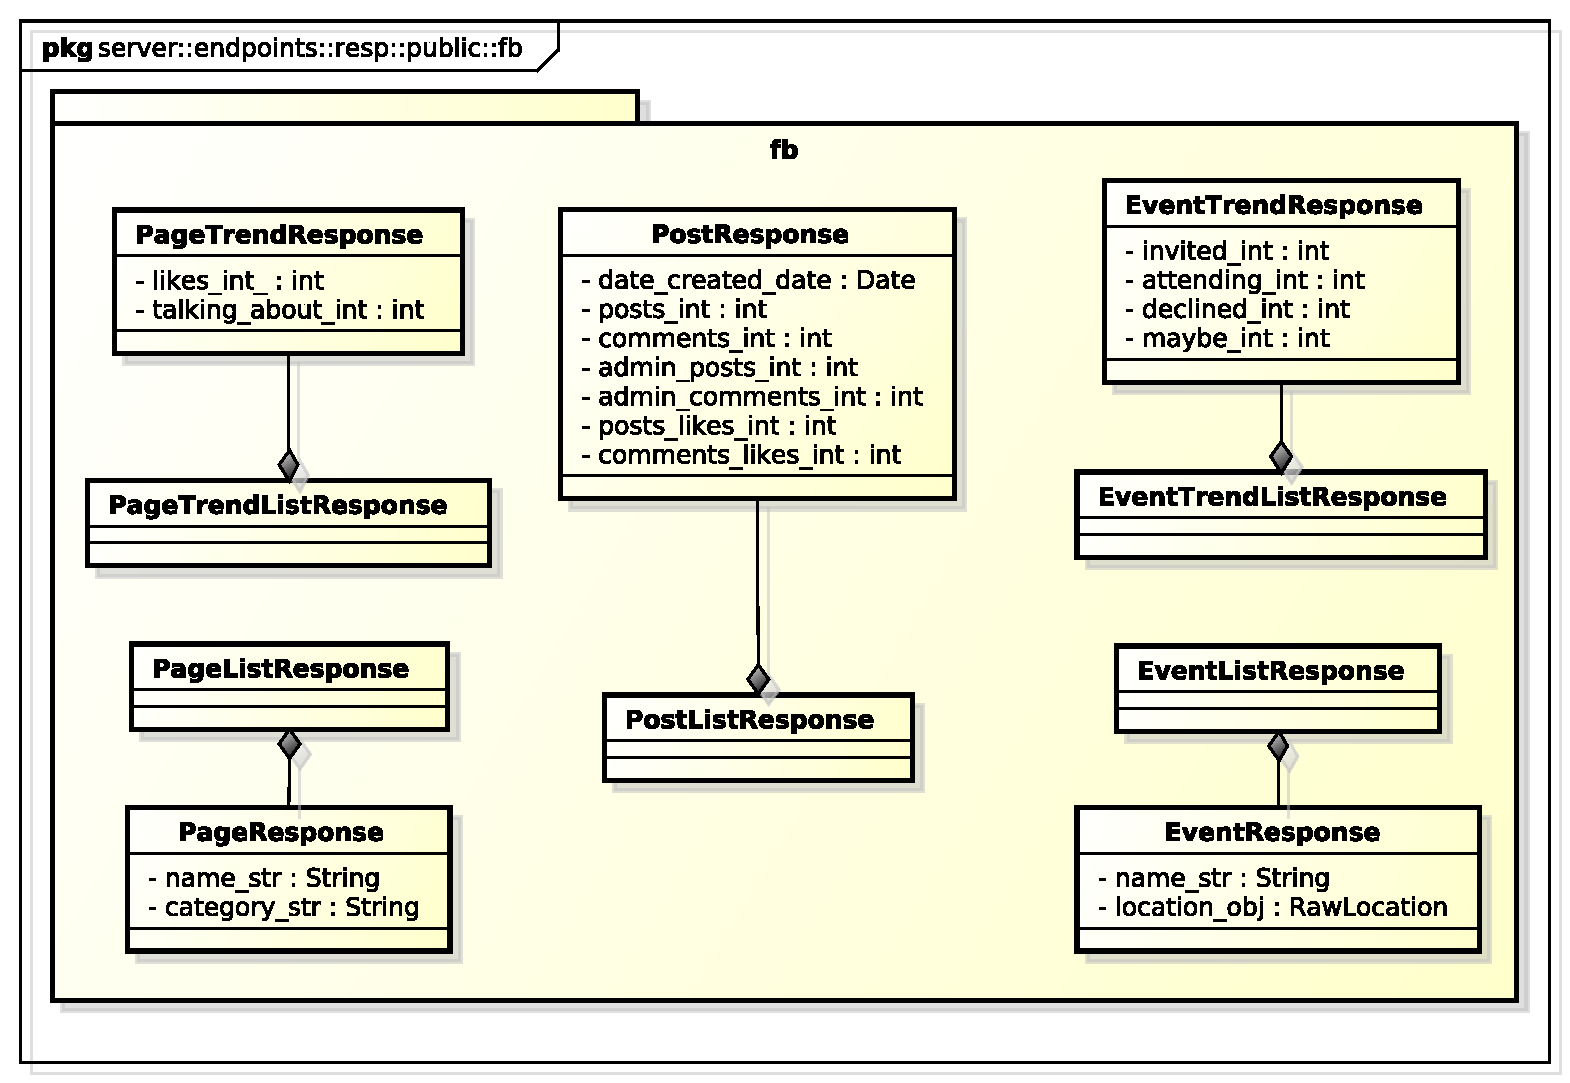
\includegraphics[scale=0.55]{./images/server/resp_fb.pdf}}
	\caption{Package - server::endpoints::resp::public::fb}
\end{figure}

\begin{itemize}
  \item \textbf{Descrizione}: è il package contenente le classi che rappresentano il modello di dati delle componenti di Facebook da restituire al client;
  \item \textbf{Padre}: server::endpoints::resp::public
  %\item \textbf{Interazione con altri componenti}:
\end{itemize}
% subsubsection

	\paragraph{Classi} % (fold)

    \subparagraph{server::endpoints::resp::public::fb::PageResponse} % (fold)
    \label{subp:bdsm_app_server_endpoints_resp_public_fb_pageresponse}
    \begin{itemize}
      \item \textbf{Descrizione}: rappresenta il modello dei dati di una pagina Facebook da ritornare al client;
      \item \textbf{Utilizzo}: viene utilizzata dalle API per restituire la response dei dati di una pagina Facebook al client;
      
	  \item \textbf{Attributi}: TO DO
	  \item \textbf{Metodi}: TO DO
      \end{itemize}
    % subparagraph bdsm_app_server_endpoints_resp_public_fb_pageresponse (end)

    \subparagraph{server::endpoints::resp::public::fb::PageListResponse} % (fold)
    \label{subp:bdsm_app_server_endpoints_resp_public_fb_pagelistresponse}
    \begin{itemize}
      \item \textbf{Descrizione}: rappresenta il modello dei dati della lista di pagine Facebook da ritornare al client;
      \item \textbf{Utilizzo}: viene utilizzata dalle API per restituire la response della lista delle pagine Facebook al client;
      \item \textbf{Relazioni con altre classi}:
        \begin{itemize}
          \item server::endpoints::resp::public::fb::PageResponse
        \end{itemize}
	  \item \textbf{Attributi}: TO DO
	  \item \textbf{Metodi}: TO DO
      \end{itemize}
    % subparagraph bdsm_app_server_endpoints_resp_public_fb_pagelistresponse (end)

    \subparagraph{server::endpoints::resp::public::fb::PageTrendResponse} % (fold)
    \label{subp:bdsm_app_server_endpoints_resp_public_fb_pagetrendresponse}
    \begin{itemize}
      \item \textbf{Descrizione}: rappresenta il modello dei dati dei trend di una pagina Facebook da ritornare al client;
      \item \textbf{Utilizzo}: viene utilizzata dalle API per restituire la response dei trend di una pagina Facebook al client;
      %\item \textbf{Relazioni con altre classi}:
	  \item \textbf{Attributi}: TO DO
	  \item \textbf{Metodi}: TO DO
    \end{itemize}
    % subparagraph bdsm_app_server_endpoints_resp_public_fb_pagetrendresponse (end)

    \subparagraph{server::endpoints::resp::public::fb::PageTrendListResponse} % (fold)
    \label{subp:bdsm_app_server_endpoints_resp_public_fb_pagetrendlistresponse}
    \begin{itemize}
      \item \textbf{Descrizione}: rappresenta il modello dei dati della lista dei trend di una pagina Facebook da ritornare al client;
      \item \textbf{Utilizzo}: viene utilizzata dalle API per restituire la response della lista dei trend di una pagina Facebook al client;
      \item \textbf{Relazioni con altre classi}:
        \begin{itemize}
          \item server::endpoints::resp::public::fb::PageTrendResponse
        \end{itemize}
	  \item \textbf{Attributi}: TO DO
	  \item \textbf{Metodi}: TO DO
      \end{itemize}
    % subparagraph bdsm_app_server_endpoints_resp_public_fb_pagetrendlistresponse (end)

    \subparagraph{server::endpoints::resp::public::fb::EventResponse} % (fold)
    \label{subp:bdsm_app_server_endpoints_resp_public_fb_eventresponse}
    \begin{itemize}
      \item \textbf{Descrizione}: rappresenta il modello dei dati di un evento di Facebook da ritornare al client;
      \item \textbf{Utilizzo}: viene utilizzata dalle API per restituire la response dei dati di un evento Facebook al client;
      
	  \item \textbf{Attributi}: TO DO
	  \item \textbf{Metodi}: TO DO
      \end{itemize}
    % subparagraph bdsm_app_server_endpoints_resp_public_fb_eventresponse (end)

    \subparagraph{server::endpoints::resp::public::fb::EventListResponse} % (fold)
    \label{subp:bdsm_app_server_endpoints_resp_public_fb_eventlistresponse}
    \begin{itemize}
      \item \textbf{Descrizione}: rappresenta il modello dei dati della lista di eventi Facebook da ritornare al client;
      \item \textbf{Utilizzo}: viene utilizzata dalle API per restituire la response della lista di eventi Facebook al client;
      \item \textbf{Relazioni con altre classi}:
        \begin{itemize}
          \item server::endpoints::resp::public::fb::EventResponse
        \end{itemize}
	  \item \textbf{Attributi}: TO DO
	  \item \textbf{Metodi}: TO DO
      \end{itemize}
    % subparagraph bdsm_app_server_endpoints_resp_public_fb_eventlistresponse (end)

    \subparagraph{server::endpoints::resp::public::fb::EventTrendResponse} % (fold)
    \label{subp:bdsm_app_server_endpoints_resp_public_fb_eventtrendresponse}
    \begin{itemize}
      \item \textbf{Descrizione}: rappresenta il modello dei dati dei trend di un evento Facebook da ritornare al client;
      \item \textbf{Utilizzo}: viene utilizzata dalle API per restituire la response dei trend di un evento Facebook al client;
      
	  \item \textbf{Attributi}: TO DO
	  \item \textbf{Metodi}: TO DO
      \end{itemize}
    % subparagraph bdsm_app_server_endpoints_resp_public_fb_eventtrendresponse (end)

    \subparagraph{server::endpoints::resp::public::fb::EventTrendListResponse} % (fold)
    \label{subp:bdsm_app_server_endpoints_resp_public_fb_eventtrendlistresponse}
    \begin{itemize}
      \item \textbf{Descrizione}: rappresenta il modello dei dati della lista dei trend di un evento Facebook da ritornare al client;
      \item \textbf{Utilizzo}: viene utilizzata dalle API per restituire la response della lista dei trend di un evento Facebook al client;
      \item \textbf{Relazioni con altre classi}:
        \begin{itemize}
          \item server::endpoints::resp::public::fb::EventTrendResponse
        \end{itemize}
	  \item \textbf{Attributi}: TO DO
	  \item \textbf{Metodi}: TO DO
      \end{itemize}
    % subparagraph bdsm_app_server_endpoints_resp_public_fb_eventtrendlistresponse (end)

    \subparagraph{server::endpoints::resp::public::fb::PostResponse} % (fold)
    \label{subp:bdsm_app_server_endpoints_resp_public_fb_postresponse}
    \begin{itemize}
      \item \textbf{Descrizione}: rappresenta il modello dei dati dei post di Facebook da ritornare al client;
      \item \textbf{Utilizzo}: viene utilizzata dalle API per restituire la response dei dati dei post Facebook al client;
      
	  \item \textbf{Attributi}: TO DO
	  \item \textbf{Metodi}: TO DO
    \end{itemize}
    % subparagraph bdsm_app_server_endpoints_resp_public_fb_postresponse (end)

    \subparagraph{server::endpoints::resp::public::fb::PostListResponse} % (fold)
    \label{subp:bdsm_app_server_endpoints_resp_public_fb_postlistresponse}
    \begin{itemize}
      \item \textbf{Descrizione}: rappresenta il modello dei dati della lista di post di Facebook da ritornare al client;
      \item \textbf{Utilizzo}: viene utilizzata dalle API per restituire la response della lista di post di Facebook al client;
      \item \textbf{Relazioni con altre classi}:
        \begin{itemize}
          \item server::endpoints::resp::public::fb::PostResponse
        \end{itemize}
	  \item \textbf{Attributi}: TO DO
	  \item \textbf{Metodi}: TO DO
      \end{itemize}
    % subparagraph bdsm_app_server_endpoints_resp_public_fb_postlistresponse (end)

\subsubsection{server::endpoints::resp::public::tw} % (fold)
\label{ssub:bdsm_app_server_endpoints_resp_public_tw}
\begin{figure}[!htbp]
	\centering
	\centerline{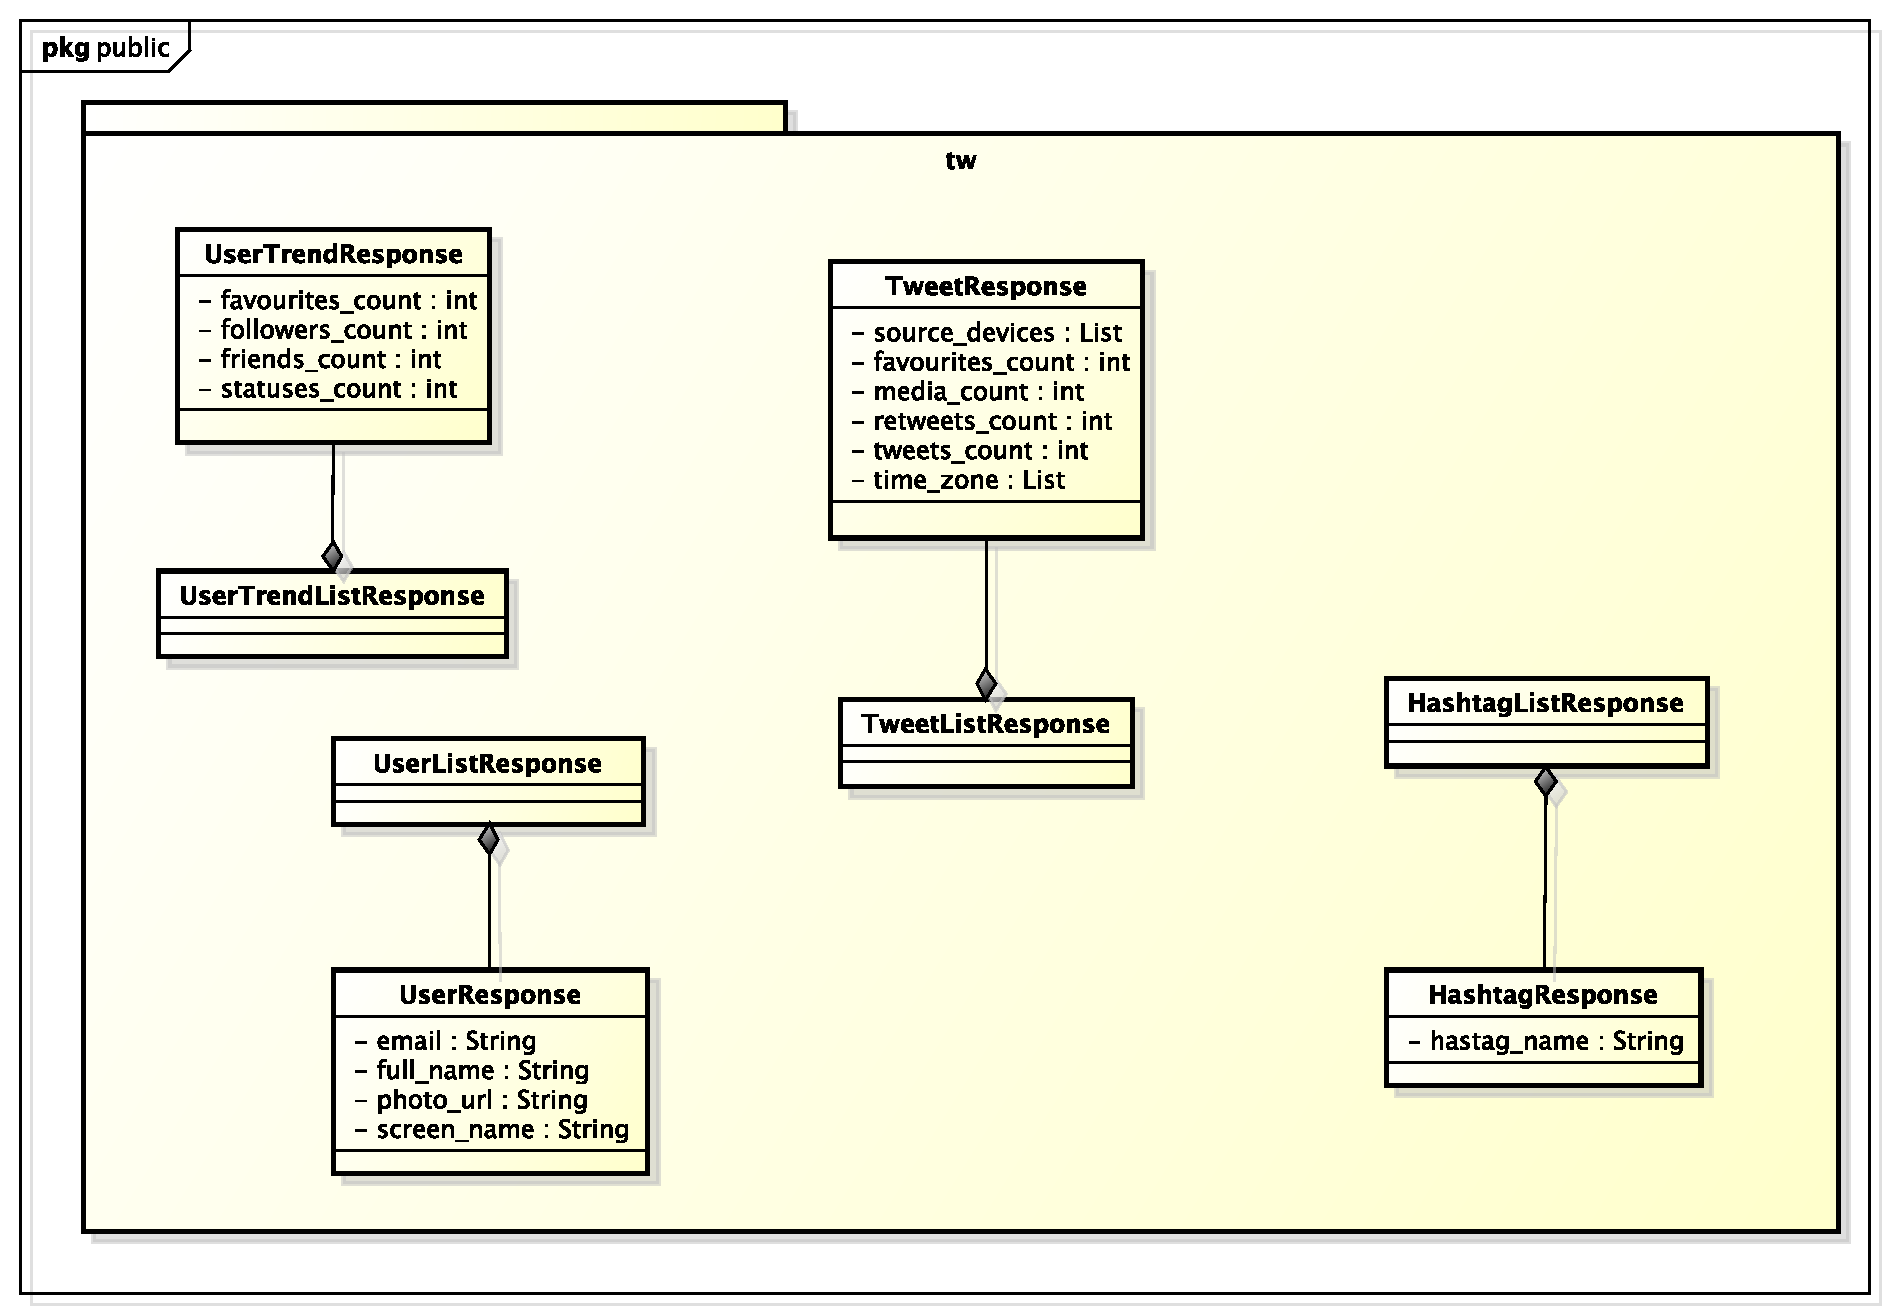
\includegraphics[scale=0.5]{./images/server/resp_tw.pdf}}
	\caption{Package - server::endpoints::resp::public::tw}
\end{figure}

\begin{itemize}
  \item \textbf{Descrizione}: è il package contenente le classi che rappresentano il modello dei dati delle componenti di Twitter da restituire al client;
  \item \textbf{Padre}: server::endpoints::resp::public
  %\item \textbf{Interazione con altri componenti}:
\end{itemize}
% subsubsection

	\paragraph{Classi} % (fold)

    \subparagraph{server::endpoints::resp::public::tw::UserResponse} % (fold)
    \label{subp:bdsm_app_server_endpoints_resp_public_tw_userresponse}
    \begin{itemize}
      \item \textbf{Descrizione}: rappresenta il modello dei dati di un profilo Twitter da ritornare al client;
      \item \textbf{Utilizzo}: viene utilizzata dalle API per restituire la response dei dati di un profilo Twitter al client;
      
	  \item \textbf{Attributi}: TO DO
	  \item \textbf{Metodi}: TO DO
      \end{itemize}
    % subparagraph bdsm_app_server_endpoints_resp_public_tw_pageresponse (end)

    \subparagraph{server::endpoints::resp::public::tw::UserListResponse} % (fold)
    \label{subp:bdsm_app_server_endpoints_resp_public_tw_userlistresponse}
    \begin{itemize}
      \item \textbf{Descrizione}: rappresenta il modello dei dati della lista di profili Twitter da ritornare al client;
      \item \textbf{Utilizzo}: viene utilizzata dalle API per restituire la response della lista di profili Twitter al client;
      \item \textbf{Relazioni con altre classi}:
        \begin{itemize}
          \item server::endpoints::resp::public::tw::UserResponse
        \end{itemize}
	  \item \textbf{Attributi}: TO DO
	  \item \textbf{Metodi}: TO DO
      \end{itemize}
    % subparagraph bdsm_app_server_endpoints_resp_public_tw_userlistresponse (end)

    \subparagraph{server::endpoints::resp::public::tw::UserTrendResponse} % (fold)
    \label{subp:bdsm_app_server_endpoints_resp_public_tw_usertrendresponse}
    \begin{itemize}
      \item \textbf{Descrizione}: rappresenta il modello dei dati dei trend di un profilo Twitter da ritornare al client;
      \item \textbf{Utilizzo}: viene utilizzata dalle API per restituire la response dei trend di un profilo Twitter al client;
      
	  \item \textbf{Attributi}: TO DO
	  \item \textbf{Metodi}: TO DO
    \end{itemize}
    % subparagraph bdsm_app_server_endpoints_resp_public_tw_usertrendresponse (end)

    \subparagraph{server::endpoints::resp::public::tw::UserTrendListResponse} % (fold)
    \label{subp:bdsm_app_server_endpoints_resp_public_tw_usertrendlistresponse}
    \begin{itemize}
      \item \textbf{Descrizione}: rappresenta il modello dei dati della lista dei trend di un profilo Twitter da ritornare al client;
      \item \textbf{Utilizzo}: viene utilizzata dalle API per restituire la response della lista dei trend di un profilo Twitter al client;
      \item \textbf{Relazioni con altre classi}:
        \begin{itemize}
          \item server::endpoints::resp::public::tw::UserTrendResponse
        \end{itemize}
	  \item \textbf{Attributi}: TO DO
	  \item \textbf{Metodi}: TO DO
    \end{itemize}
    % subparagraph bdsm_app_server_endpoints_resp_public_tw_usertrendlistresponse (end)

    \subparagraph{server::endpoints::resp::public::tw::HashtagResponse} % (fold)
    \label{subp:bdsm_app_server_endpoints_resp_public_tw_hashtagresponse}
    \begin{itemize}
      \item \textbf{Descrizione}: rappresenta il modello dei dati di un hashtag di Twitter da ritornare al client;
      \item \textbf{Utilizzo}: viene utilizzata dalle API per restituire la response dei dati di un hashtag di Twitter al client;
      
	  \item \textbf{Attributi}: TO DO
	  \item \textbf{Metodi}: TO DO
    \end{itemize}
    % subparagraph bdsm_app_server_endpoints_resp_public_tw_hashtagresponse (end)

    \subparagraph{server::endpoints::resp::public::tw::HashtagListResponse} % (fold)
    \label{subp:bdsm_app_server_endpoints_resp_public_tw_hashtaglistresponse}
    \begin{itemize}
      \item \textbf{Descrizione}: rappresenta il modello dei dati della lista degli hashtag di Twitter da ritornare al client;
      \item \textbf{Utilizzo}: viene utilizzata dalle API per restituire la response della lista degli hashtag di Twitter al client;
      \item \textbf{Relazioni con altre classi}:
        \begin{itemize}
          \item server::endpoints::resp::public::tw::HashtagResponse
        \end{itemize}
	  \item \textbf{Attributi}: TO DO
	  \item \textbf{Metodi}: TO DO
      \end{itemize}
    % subparagraph bdsm_app_server_endpoints_resp_public_tw_hashtaglistresponse (end)

    \subparagraph{server::endpoints::resp::public::tw::TweetResponse} % (fold)
    \label{subp:bdsm_app_server_endpoints_resp_public_tw_tweetresponse}
    \begin{itemize}
      \item \textbf{Descrizione}: rappresenta il modello dei dati dei tweet di Twitter da ritornare al client;
      \item \textbf{Utilizzo}: viene utilizzata dalle API per restituire la response dei dati dei tweet di Twitter al client;
      
	  \item \textbf{Attributi}: TO DO
	  \item \textbf{Metodi}: TO DO
    \end{itemize}
    % subparagraph bdsm_app_server_endpoints_resp_public_tw_tweetresponse (end)

    \subparagraph{server::endpoints::resp::public::tw::TweetListResponse} % (fold)
    \label{subp:bdsm_app_server_endpoints_resp_public_tw_tweetlistresponse}
    \begin{itemize}
      \item \textbf{Descrizione}: rappresenta il modello dei dati della lista dei tweet Twitter da ritornare al client;
      \item \textbf{Utilizzo}: viene utilizzata dalle API per restituire la response della lista dei tweet di Twitter al client;
      \item \textbf{Relazioni con altre classi}:
        \begin{itemize}
          \item server::endpoints::resp::public::tw::TweetResponse
        \end{itemize}
	  \item \textbf{Attributi}: TO DO
	  \item \textbf{Metodi}: TO DO
    \end{itemize}
    % subparagraph bdsm_app_server_endpoints_resp_public_tw_tweetlistresponse (end)

\subsubsection{server::endpoints::resp::public::ig} % (fold)
\label{ssub:bdsm_app_server_endpoints_resp_public_ig}
\begin{figure}[!htbp]
	\centering
	\centerline{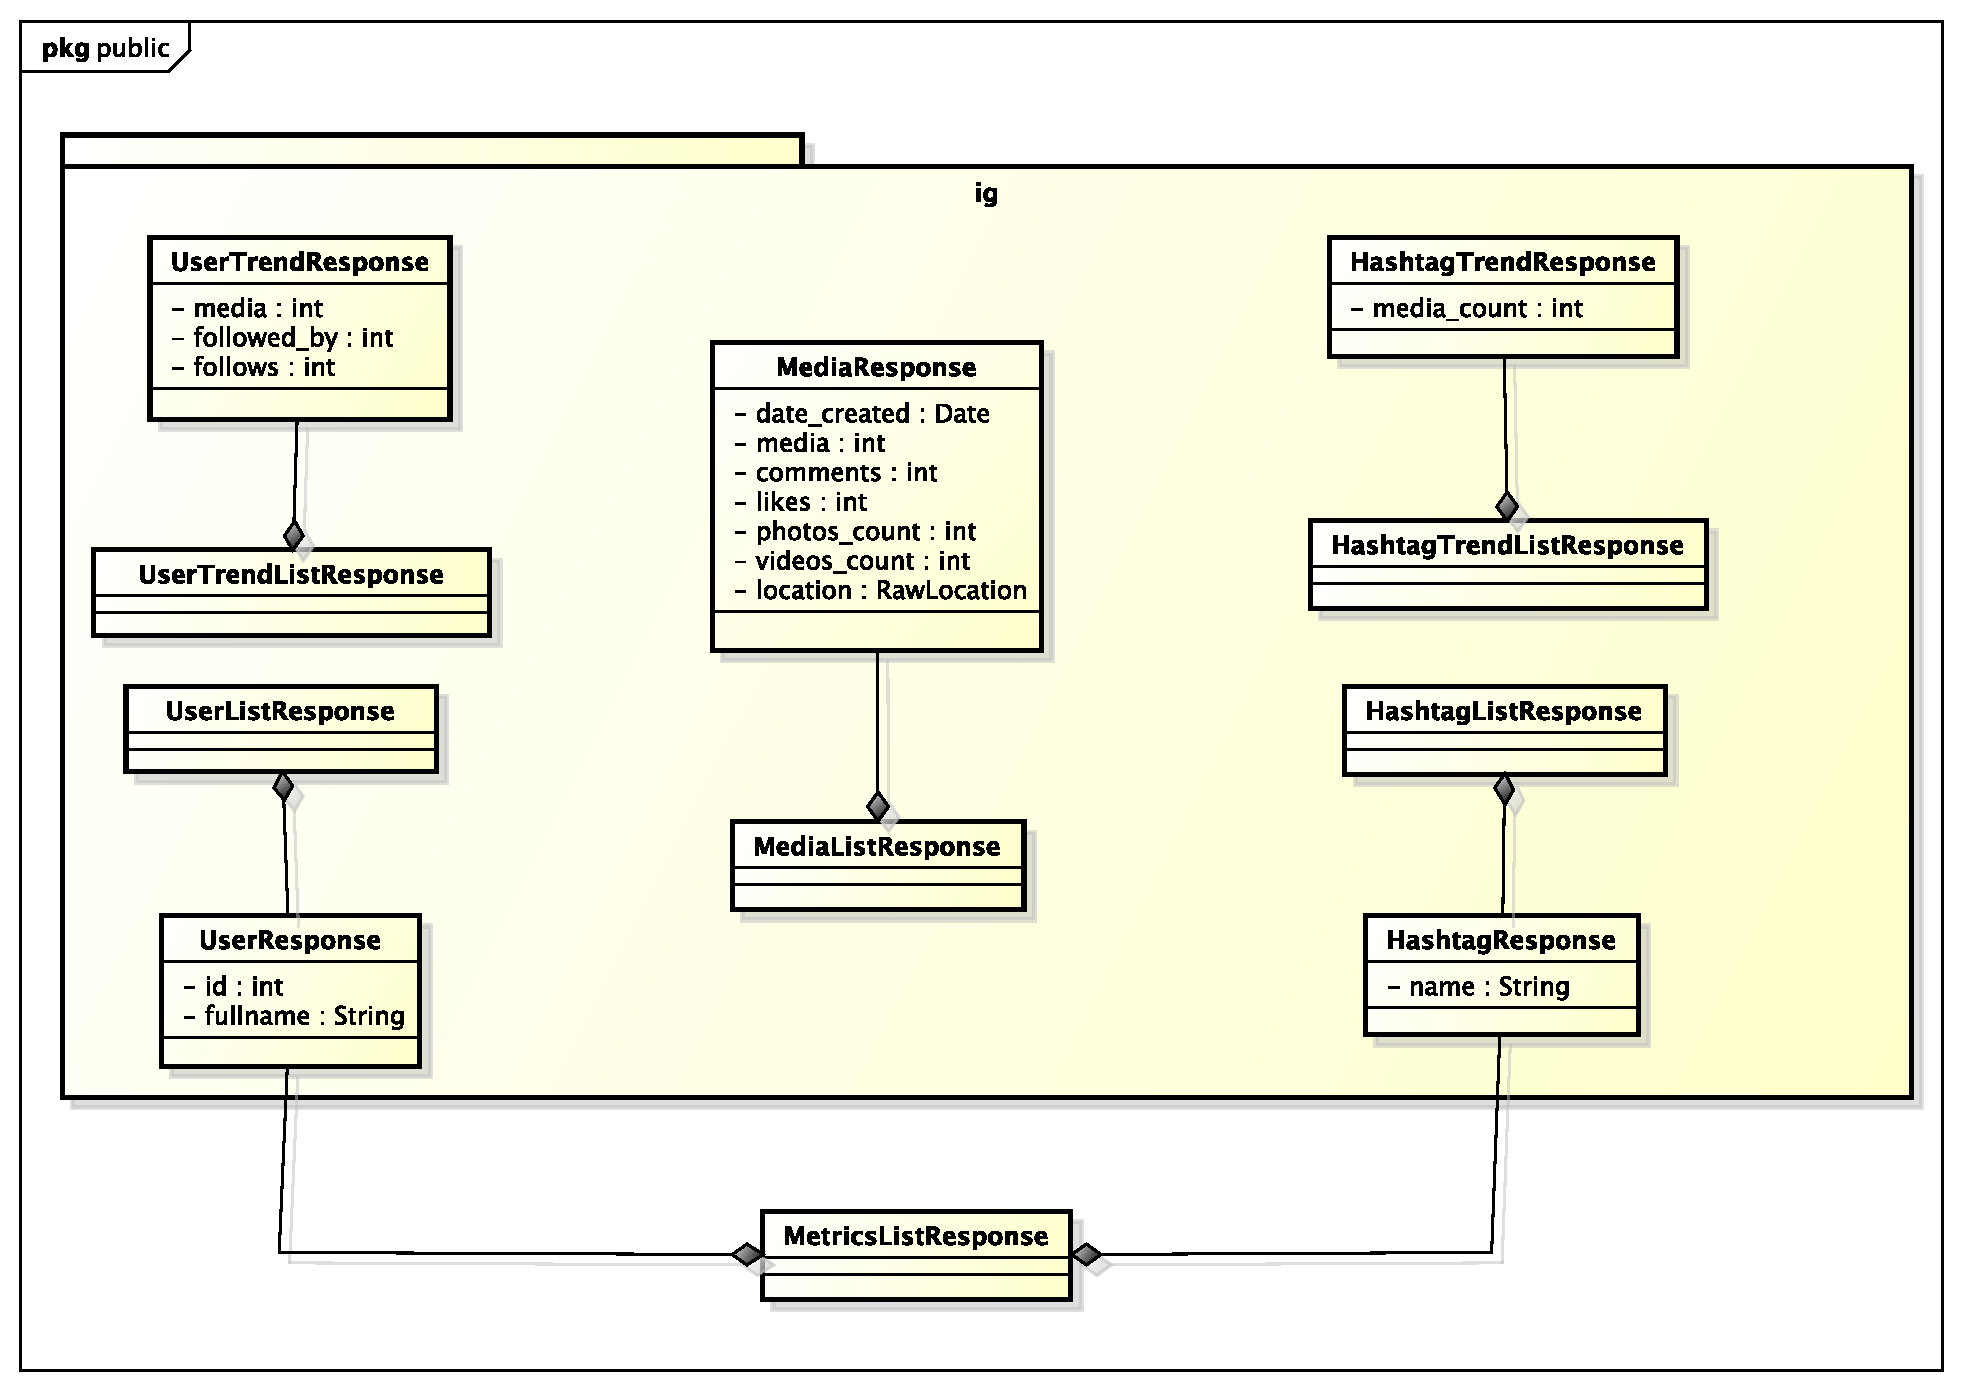
\includegraphics[scale=0.5]{./images/server/resp_ig.pdf}}
	\caption{Package - server::endpoints::resp::public::ig}
\end{figure}

\begin{itemize}
  \item \textbf{Descrizione}: è il package contenente le classi che rappresentano il modello dei dati delle componenti di Instagram da restituire al client;
  \item \textbf{Padre}: server::endpoints::resp::public
  %\item \textbf{Interazione con altri componenti}:
\end{itemize}
% subsubsection

	\paragraph{Classi} % (fold)

    \subparagraph{server::endpoints::resp::public::ig::UserResponse} % (fold)
    \label{subp:bdsm_app_server_endpoints_resp_public_ig_userresponse}
    \begin{itemize}
      \item \textbf{Descrizione}: rappresenta il modello dei dati di un profilo Instagram da ritornare al client;
      \item \textbf{Utilizzo}: viene utilizzata dalle API per restituire la response dei dati di un profilo Instagram al client;
      
	  \item \textbf{Attributi}: TO DO
	  \item \textbf{Metodi}: TO DO
      \end{itemize}
    % subparagraph bdsm_app_server_endpoints_resp_public_ig_pageresponse (end)

    \subparagraph{server::endpoints::resp::public::ig::UserListResponse} % (fold)
    \label{subp:bdsm_app_server_endpoints_resp_public_ig_userlistresponse}
    \begin{itemize}
      \item \textbf{Descrizione}: rappresenta il modello dei dati della lista dei profili di Instagram da ritornare al client;
      \item \textbf{Utilizzo}: viene utilizzata dalle API per restituire la response della lista dei profili di Instagram al client;
      \item \textbf{Relazioni con altre classi}:
        \begin{itemize}
          \item server::endpoints::resp::public::ig::UserResponse
        \end{itemize}
	  \item \textbf{Attributi}: TO DO
	  \item \textbf{Metodi}: TO DO
      \end{itemize}
    % subparagraph bdsm_app_server_endpoints_resp_public_ig_userlistresponse (end)

    \subparagraph{server::endpoints::resp::public::ig::UserTrendResponse} % (fold)
    \label{subp:bdsm_app_server_endpoints_resp_public_ig_usertrendresponse}
    \begin{itemize}
      \item \textbf{Descrizione}: rappresenta il modello dei dati dei trend di un profilo Instagram da ritornare al client;
      \item \textbf{Utilizzo}: viene utilizzata dalle API per restituire la response dei trend di un profilo Instagram al client;
      
	  \item \textbf{Attributi}: TO DO
	  \item \textbf{Metodi}: TO DO
      \end{itemize}
    % subparagraph bdsm_app_server_endpoints_resp_public_ig_usertrendresponse (end)

    \subparagraph{server::endpoints::resp::public::ig::UserTrendListResponse} % (fold)
    \label{subp:bdsm_app_server_endpoints_resp_public_ig_usertrendlistresponse}
    \begin{itemize}
      \item \textbf{Descrizione}: rappresenta il modello dei dati della lista dei trend di un profilo Instagram da ritornare al client;
      \item \textbf{Utilizzo}: viene utilizzata dalle API per restituire la response della lista dei trend di un profilo Instagram al client;
      \item \textbf{Relazioni con altre classi}:
        \begin{itemize}
          \item server::endpoints::resp::public::ig::UserTrendResponse
        \end{itemize}
	  \item \textbf{Attributi}: TO DO
	  \item \textbf{Metodi}: TO DO
      \end{itemize}
    % subparagraph bdsm_app_server_endpoints_resp_public_ig_usertrendlistresponse (end)

    \subparagraph{server::endpoints::resp::public::ig::HashtagResponse} % (fold)
    \label{subp:bdsm_app_server_endpoints_resp_public_ig_hashtagresponse}
    \begin{itemize}
      \item \textbf{Descrizione}: rappresenta il modello dei dati di un hashtag di Instagram da ritornare al client;
      \item \textbf{Utilizzo}: viene utilizzata dalle API per restituire la response dei dati di un hashtag di Instagram al client;
      
	  \item \textbf{Attributi}: TO DO
	  \item \textbf{Metodi}: TO DO
      \end{itemize}
    % subparagraph bdsm_app_server_endpoints_resp_public_ig_hashtagresponse (end)

    \subparagraph{server::endpoints::resp::public::ig::HashtagListResponse} % (fold)
    \label{subp:bdsm_app_server_endpoints_resp_public_ig_hashtaglistresponse}
    \begin{itemize}
      \item \textbf{Descrizione}: rappresenta il modello dei dati della lista degli hashtag di Instagram da ritornare al client;
      \item \textbf{Utilizzo}: viene utilizzata dalle API per restituire la response della lista degli hashtag di Instagram al client;
      \item \textbf{Relazioni con altre classi}:
        \begin{itemize}
          \item server::endpoints::resp::public::ig::HashtagResponse
        \end{itemize}
	  \item \textbf{Attributi}: TO DO
	  \item \textbf{Metodi}: TO DO
      \end{itemize}
    % subparagraph bdsm_app_server_endpoints_resp_public_ig_hashtaglistresponse (end)

    \subparagraph{server::endpoints::resp::public::ig::HashtagTrendResponse} % (fold)
    \label{subp:bdsm_app_server_endpoints_resp_public_ig_hashtagtrendresponse}
    \begin{itemize}
      \item \textbf{Descrizione}: rappresenta il modello dei dati dei trend di un hashtag di Instagram da ritornare al client;
      \item \textbf{Utilizzo}: viene utilizzata dalle API per restituire la response dei trend di un hashtag di Instagram al client;
      
	  \item \textbf{Attributi}: TO DO
	  \item \textbf{Metodi}: TO DO
      \end{itemize}
    % subparagraph bdsm_app_server_endpoints_resp_public_ig_hashtagtrendresponse (end)

    \subparagraph{server::endpoints::resp::public::ig::HashtagTrendListResponse} % (fold)
    \label{subp:bdsm_app_server_endpoints_resp_public_ig_hashtagtrendlistresponse}
    \begin{itemize}
      \item \textbf{Descrizione}: rappresenta il modello dei dati della lista dei trend di un hashtag di Instagram da ritornare al client;
      \item \textbf{Utilizzo}: viene utilizzata dalle API per restituire la response della lista dei trend di un hashtag di Instagram al client;
      \item \textbf{Relazioni con altre classi}:
        \begin{itemize}
          \item server::endpoints::resp::public::ig::HashtagTrendResponse
        \end{itemize}
	  \item \textbf{Attributi}: TO DO
	  \item \textbf{Metodi}: TO DO
      \end{itemize}
    % subparagraph bdsm_app_server_endpoints_resp_public_ig_hashtagtrendlistresponse (end)

    \subparagraph{server::endpoints::resp::public::ig::MediaResponse} % (fold)
    \label{subp:bdsm_app_server_endpoints_resp_public_ig_mediaresponse}
    \begin{itemize}
      \item \textbf{Descrizione}: rappresenta il modello dei dati dei media di Instagram da ritornare al client;
      \item \textbf{Utilizzo}: viene utilizzata dalle API per restituire la response dei dati dei media di Instagram al client;
      
	  \item \textbf{Attributi}: TO DO
	  \item \textbf{Metodi}: TO DO
      \end{itemize}
    % subparagraph bdsm_app_server_endpoints_resp_public_ig_mediaresponse (end)

    \subparagraph{server::endpoints::resp::public::ig::MediaListResponse} % (fold)
    \label{subp:bdsm_app_server_endpoints_resp_public_ig_medialistresponse}
    \begin{itemize}
      \item \textbf{Descrizione}: rappresenta il modello dei dati della lista dei media di Instagram da ritornare al client;
      \item \textbf{Utilizzo}: viene utilizzata dalle API per restituire la response della lista dei media di Instagram al client;
      \item \textbf{Relazioni con altre classi}:
        \begin{itemize}
          \item server::endpoints::resp::public::ig::MediaResponse
        \end{itemize}
	  \item \textbf{Attributi}: TO DO
	  \item \textbf{Metodi}: TO DO
      \end{itemize}
    % subparagraph bdsm_app_server_endpoints_resp_public_ig_medialistresponse (end)

\subsubsection{server::endpoints::resp::private} % (fold)
\label{ssub:bdsm_app_server_endpoints_resp_private}
\begin{figure}[!htbp]
	\centering
	\centerline{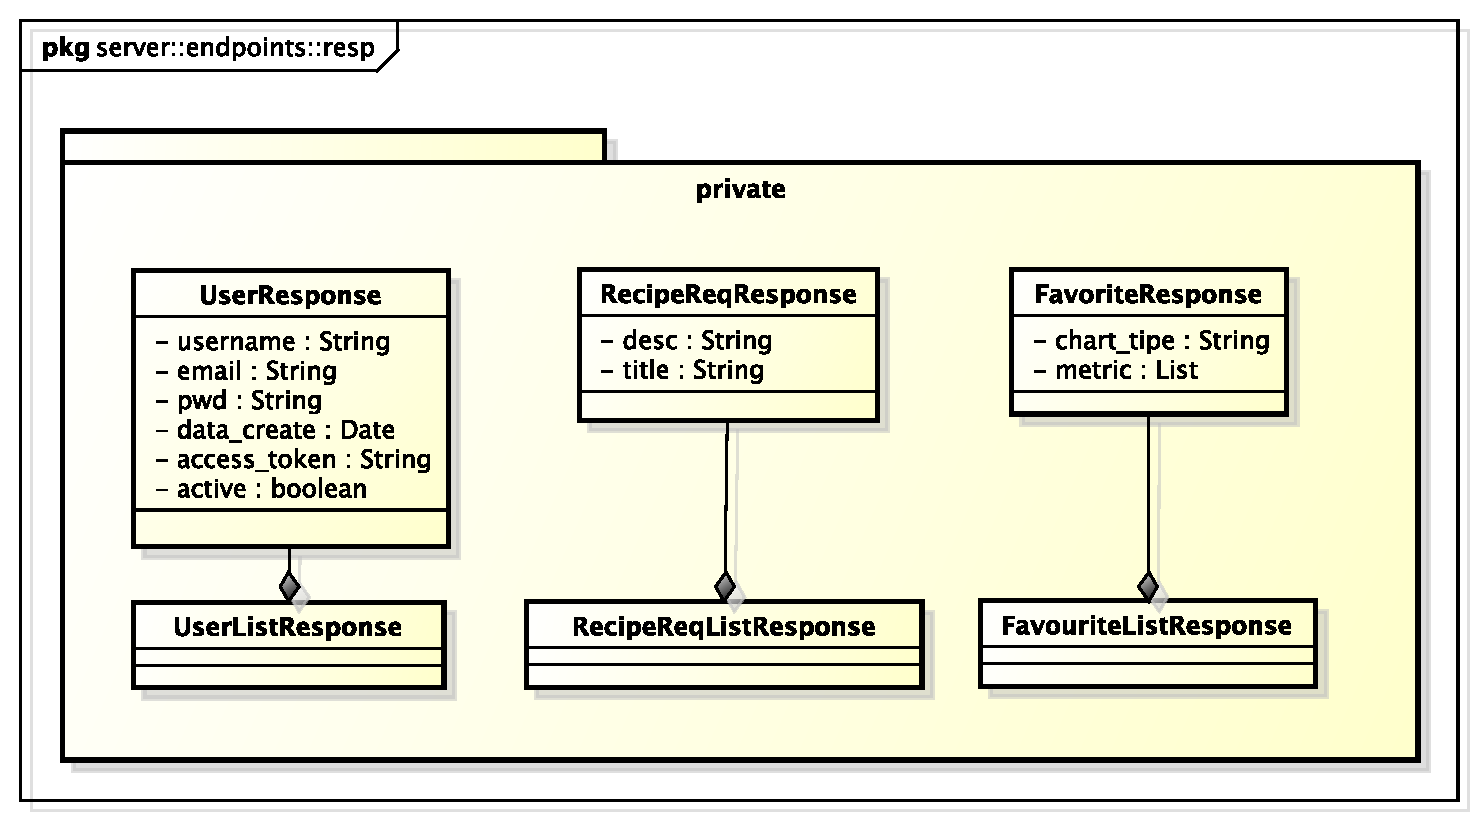
\includegraphics[scale=0.45]{./images/server/resp_private.pdf}}
	\caption{Package - server::endpoints::resp::private}
\end{figure}

\begin{itemize}
  \item \textbf{Descrizione}: è il package che definisce i modelli delle risposte da passare al client in seguito alle chiamate API;
  \item \textbf{Padre}: server::endpoints::resp
  \item \textbf{Interazione con altri componenti}:
  	\begin{itemize}
  		\item server::endpoints::resp::public
	\end{itemize}
\end{itemize}
% subsubsection

	\paragraph{Classi} % (fold)

    \subparagraph{server::endpoints::resp::private::RecipeResponse} % (fold)
    \label{subp:bdsm_app_server_endpoints_resp_private_reciperesponse}
    \begin{itemize}
      \item \textbf{Descrizione}: rappresenta il modello dei dati di una Recipe da ritornare al client;
      \item \textbf{Utilizzo}: viene utilizzata dalle API per restituire la response di una Recipe al client;
      \item \textbf{Relazioni con altre classi}:
        \begin{itemize}
  			\item server::endpoints::resp::public::MetricListResponse
		\end{itemize}
	  \item \textbf{Attributi}: TO DO
	  \item \textbf{Metodi}: TO DO
      \end{itemize}
    % subparagraph bdsm_app_server_endpoints_resp_private_reciperesponse (end)

    \subparagraph{server::endpoints::resp::private::RecipeListResponse} % (fold)
    \label{subp:bdsm_app_server_endpoints_resp_private_recipelistresponse}
    \begin{itemize}
      \item \textbf{Descrizione}: rappresenta il modello dei dati di una Recipe da ritornare al client;
      \item \textbf{Utilizzo}: viene utilizzata dalle API per restituire la response di una Recipe al client;
      \item \textbf{Relazioni con altre classi}:
        \begin{itemize}
          \item server::endpoints::resp::private::RecipeResponse
        \end{itemize}
	  \item \textbf{Attributi}: TO DO
	  \item \textbf{Metodi}: TO DO
      \end{itemize}
    % subparagraph bdsm_app_server_endpoints_resp_private_recipelistresponse (end)

    \subparagraph{server::endpoints::resp::private::RecipeReqResponse} % (fold)
    \label{subp:bdsm_app_server_endpoints_resp_private_recipereqresponse}
    \begin{itemize}
      \item \textbf{Descrizione}: rappresenta il modello dei dati di una richiesta di Recipe da ritornare al client;
      \item \textbf{Utilizzo}: viene utilizzata dalle API per restituire la response di una richiesta di Recipe al client;
	  \item \textbf{Attributi}: TO DO
	  \item \textbf{Metodi}: TO DO
      \end{itemize}
    % subparagraph bdsm_app_server_endpoints_resp_private_recipereqresponse (end)

    \subparagraph{server::endpoints::resp::private::RecipeReqListResponse} % (fold)
    \label{subp:bdsm_app_server_endpoints_resp_private_recipereqlistresponse}
    \begin{itemize}
      \item \textbf{Descrizione}: rappresenta il modello dei dati di una lista di richieste di Recipe da ritornare al client;
      \item \textbf{Utilizzo}: viene utilizzata dalle API per restituire la response di una lista di richieste di Recipe al client;
      \item \textbf{Relazioni con altre classi}:
        \begin{itemize}
          \item server::endpoints::resp::private::RecipeReqResponse
        \end{itemize}
	  \item \textbf{Attributi}: TO DO
	  \item \textbf{Metodi}: TO DO
      \end{itemize}
    % subparagraph bdsm_app_server_endpoints_resp_private_recipereqlistresponse (end)

    \subparagraph{server::endpoints::resp::private::UserResponse} % (fold)
    \label{subp:bdsm_app_server_endpoints_resp_private_userresponse}
    \begin{itemize}
      \item \textbf{Descrizione}: rappresenta il modello dei dati di un utente da ritornare al client;
      \item \textbf{Utilizzo}: viene utilizzata dalle API per restituire la response contenente i dati un un utente al client;
	  \item \textbf{Attributi}: TO DO
	  \item \textbf{Metodi}: TO DO
    \end{itemize}
    % subparagraph bdsm_app_server_endpoints_resp_private_userresponse (end)
    
    \subparagraph{server::endpoints::resp::private::UserListResponse} % (fold)
    \label{subp:bdsm_app_server_endpoints_resp_private_userlistresponse}
    \begin{itemize}
      \item \textbf{Descrizione}: rappresenta il modello dei dati della lista degli utenti registrati da ritornare al client;
      \item \textbf{Utilizzo}: viene utilizzata dalle API per restituire la response della lista degli utenti al client;
	  \item \textbf{Attributi}: TO DO
	  \item \textbf{Metodi}: TO DO
    \end{itemize}
    % subparagraph bdsm_app_server_endpoints_resp_private_userlistresponse (end)

    \subparagraph{server::endpoints::resp::private::FavoriteResponse} % (fold)
    \label{subp:bdsm_app_server_endpoints_resp_private_favoriteresponse}
    \begin{itemize}
      \item \textbf{Descrizione}: rappresenta il modello dei dati di una View preferita da ritornare al client;
      \item \textbf{Utilizzo}: viene utilizzata dalle API per restituire la response di una View preferita al client;
	  \item \textbf{Attributi}: TO DO
	  \item \textbf{Metodi}: TO DO
    \end{itemize}
    % subparagraph bdsm_app_server_endpoints_resp_private_favoriteresponse (end)

    \subparagraph{server::endpoints::resp::private::FavoriteListResponse} % (fold)
    \label{subp:bdsm_app_server_endpoints_resp_private_favoritelistresponse}
    \begin{itemize}
      \item \textbf{Descrizione}: rappresenta il modello dei dati di una lista di View preferite da ritornare al client;
      \item \textbf{Utilizzo}: viene utilizzata dalle API per restituire la response di una lista di View preferite al client;
      \item \textbf{Relazioni con altre classi}:
        \begin{itemize}
          \item server::endpoints::resp::private::FavoriteResponse
        \end{itemize}
	  \item \textbf{Attributi}: TO DO
	  \item \textbf{Metodi}: TO DO
      \end{itemize}
    % subparagraph bdsm_app_server_endpoints_resp_private_favoritelistresponse (end)
 \clearpage \newpage
  % END PACKAGE ENDPOINTS


% TEMPLATE PER IL PACKAGE
%	\begin{comment}
%	\subsubsection{Nome package} % (fold)
%	\label{ssub:nome_del_package}
%	[TO DO] (diagramma) \newline \newline

%	\begin{itemize}
%		\item \textbf{Descrizione}: [TO DO];
%		\item \textbf{Padre}: [TO DO] (qualora presente);
%		\item \textbf{Package contenuti}: [TO DO] (qualora presente);
%		\item \textbf{Interazione con altri componenti}: [TO DO];
%	\end{itemize}

%		\paragraph{Classi} % (fold)
%			\subparagraph{Nome package::Nome classe} % (fold)
%			\label{subp:subparagraph_name}
%				\begin{itemize}
%					\item \textbf{Descrizione}: [TO DO];
%					\item \textbf{Utilizzo}: [TO DO];
%					\item \textbf{Classi ereditate}: [TO DO];
%					\item \textbf{Relazioni con altre classi}: [TO DO].
%				\end{itemize}
    % subparagraph subparagraph_name (end)
%	\end{comment}
    % subsection nome_classe (end)

  % paragraph classi (end)
% subsubsection nome_del_package (end)

% subsection client (end)
